\documentclass{ieeeaccess}
\usepackage{cite}
\usepackage{amsmath,amssymb,amsfonts}
\usepackage{algorithmic}
\usepackage{graphicx}
\usepackage{textcomp}
\usepackage{makecell}
\usepackage{booktabs}
\usepackage{float}
\usepackage{subcaption}
\usepackage{xcolor}
\usepackage{soul}
\usepackage{framed}
\definecolor{rtwo}{rgb}{1.0, 0.7, 0.7}
\newcommand{\hltwo}[1]{{\sethlcolor{rtwo}\hl{#1}}}
\newenvironment{rtwohl}
  {\def\FrameCommand{\colorbox{rtwo}}\MakeFramed{\advance\hsize-\width\FrameRestore}}
  {\endMakeFramed}
\definecolor{rthree}{rgb}{0.7, 0.85, 1.0}
\newcommand{\hlthree}[1]{{\sethlcolor{rthree}\hl{#1}}}
\newenvironment{rthreehl}
  {\def\FrameCommand{\colorbox{rthree}}\MakeFramed{\advance\hsize-\width\FrameRestore}}
  {\endMakeFramed}
\definecolor{roverlap}{rgb}{0.7, 1.0, 0.7}
\newcommand{\hloverlap}[1]{{\sethlcolor{roverlap}\hl{#1}}}
\newenvironment{roverlaphl}
  {\def\FrameCommand{\colorbox{roverlap}}\MakeFramed{\advance\hsize-\width\FrameRestore}}
  {\endMakeFramed}
\usepackage{hyperref}
\usepackage{varioref}
\usepackage{cleveref}
\hypersetup{colorlinks=true,linkcolor=black,citecolor=black,urlcolor=black}

% Improved float placement settings
\setlength{\textfloatsep}{10pt plus 2pt minus 2pt}
\setlength{\intextsep}{10pt plus 2pt minus 2pt}
\setlength{\floatsep}{10pt plus 2pt minus 2pt}

% Allow more floats per page
\renewcommand{\topfraction}{0.9}
\renewcommand{\bottomfraction}{0.8}
\renewcommand{\textfraction}{0.1}
\renewcommand{\floatpagefraction}{0.8}
\setcounter{topnumber}{3}
\setcounter{bottomnumber}{3}
\setcounter{totalnumber}{5}

\def\BibTeX{{\rm B\kern-.05em{\sc i\kern-.025em b}\kern-.08em
    T\kern-.1667em\lower.7ex\hbox{E}\kern-.125emX}}
\begin{document}
\history{Date of publication xxxx 00, 0000, date of current version xxxx 00, 0000.}
\doi{10.1109/ACCESS.2017.DOI}

\title{Benchmarking  Deep Reinforcement Learning for Cartesian Path Tracking  of Free-Floating Space Robot Manipulators}
\author{\uppercase{Patrick S. Ermisch}\authorrefmark{1}, and 
\uppercase{Eric Guiffo Kaigom\authorrefmark{1}} }
\address[1]{Department of Computer Science \& Engineering, Frankfurt University of Applied Sciences, Frankfurt am Main, Germany \\(e-mail: steven.ermisch@stud.fra-uas.de, kaigom@fra-uas.de)}
%\address[2]{Department of Physics, Colorado State University, Fort Collins, 
%CO 80523 USA (e-mail: author@lamar.colostate.edu)
%}
%\tfootnote{This paragraph of the first footnote will contain support  information, including sponsor and financial support acknowledgment. For example, ``This work was supported in part by the U.S. Department of Commerce under Grant BS123456.''}

\markboth
{P. S. Ermisch and E. G. Kaigom: Safe RL for Free-Floating Space Robot Manipulators}
{P. S. Ermisch and E. G. Kaigom: Safe RL for Free-Floating Space Robot Manipulators}

\corresp{Corresponding author: Eric Guiffo Kaigom (e-mail: kaigom@fra-uas.de).}

\begin{abstract}
Free-floating space robots exhibit a strong dynamic coupling between manipulator motion and base attitude disturbance,
which complicates Cartesian path tracking of the end-effector.
Supervised data-driven motion control approaches are difficult to apply because labelled data from on-orbit 
operations are scarce. This paper therefore investigates reinforcement learning for Cartesian path tracking 
of free-floating space robots in a physics-based Simulink/Simscape environment with integrated safety monitoring. 
Because a unified quantitative and qualitative comparison of these methods is currently lacking for on-orbit 
servicing, six RL algorithms are benchmarked: TRPO, TD3, SAC, PPO, PG, and DDPG. Their performance is evaluated 
using a unified set of key performance indicators covering training duration and stability, tracking 
accuracy, base attitude disturbance, motion smoothness, energy consumption, and collision risk. Among the six 
algorithms, PPO yields the best trade-off between tracking accuracy, base disturbance minimization, and training stability.
The effect of a systematic tuning of the neural network architecture and the key hyperparameters of PPO is then 
quantified for tracking both circular and piecewise-linear Cartesian paths.
Compared with the default PPO configuration, the optimized version improves the mean episodic return 
from $-2.23$ to $-0.43$, reduces the mean squared tracking error by 67.7\% and the maximum tracking error by 
44.1\%, and reduces the base orientation error by 67.0\%. In the 30 evaluation episodes considered, no 
collisions or joint-limit violations are observed for the optimized PPO agent, and the energy consumption is 
reduced by 15.98\%.
\end{abstract}

\begin{keywords}
Free-floating on-orbit servicing, Proximal Policy Optimization (PPO), reinforcement learning, 
safe simulation, space robotics,  trajectory tracking
\end{keywords}

\titlepgskip=-15pt

\maketitle

\section{Introduction and Background}

\begin{figure}[!t]
	\centering
	\begin{subfigure}{0.99\columnwidth}
		\centering
		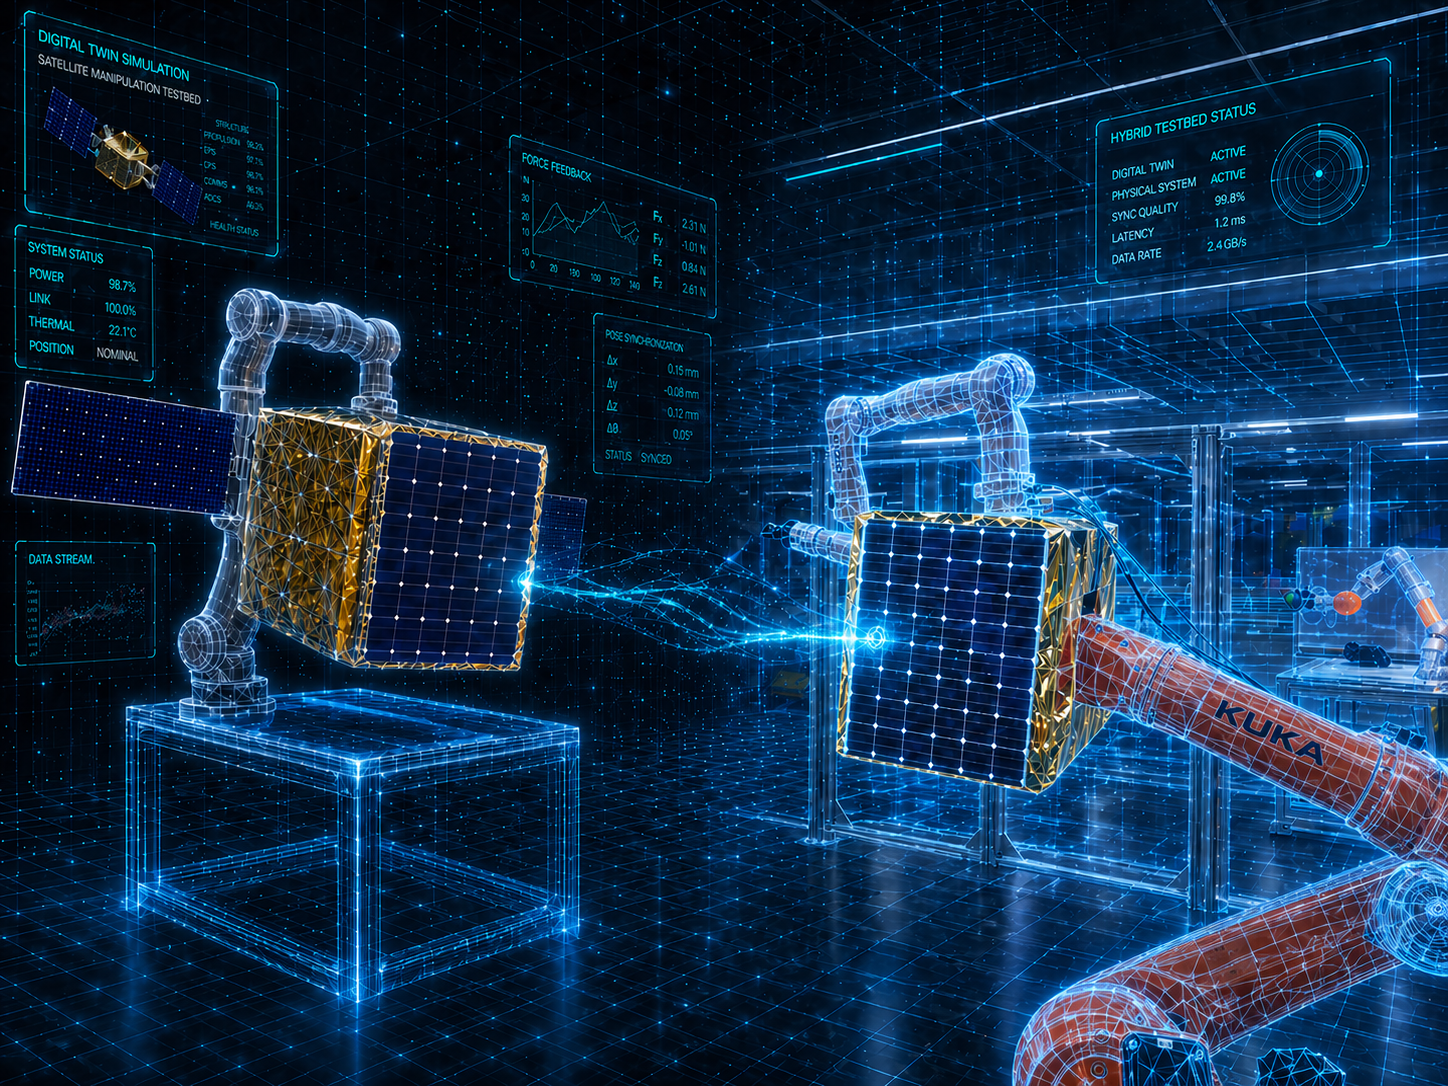
\includegraphics[width=\linewidth]{Figures/oos0.png}
	\end{subfigure}
	\caption{Virtual testbeds based on AI-driven digital twins support the safe and repeatable
  development of learning-based control methods for in-space operations under realistic yet controllable
  conditions. Illustration created using a picture of the physical setup 
  and with the help of GPT-Image-2.}
	\label{fig:oos0}
\end{figure}

Free-floating robot manipulators operating in space for satellite inspection, capture, or de-orbiting 
introduce control challenges not encountered with terrestrial robots \cite{b1}.
In micro-gravity, the robot's base (typically a spacecraft) is not fixed and the thrusters are inactive.
Manipulator motions therefore change the position and orientation of the base, which in turn modifies the 
pose of the end-effector. This reaction is a consequence of the conservation of
linear and angular momentum \cite{b6}. Operating the manipulator under free-floating dynamics avoids the 
consumption of propellant (e.g.\ hydrazine, $\mathrm{N_2H_4}$) and the excitation of structural modes by 
the pulse-width modulation of thruster control at certain frequencies \cite{b11}. This extends the operational 
lifetime of the spacecraft and supports mission success.


However, a free-floating base complicates manipulator control.
Standard motion-planning approaches developed for fixed-base robots can fail to drive the end-effector to 
the desired target. Additional constraints, such as communication latency
and limited onboard computational resources, further complicate continuous real-time control and base 
stabilization \cite{b1,b32}. Model-based approaches that assume an accurate dynamic model (e.g.\ reactionless 
planning or precise attitude control)
are sensitive to model uncertainty and unmodelled dynamics. Supervised data-driven approaches are also 
difficult to apply because
labelled training data of sufficient amount and quality are typically unavailable in the space sector.
In addition, tracking capability under a free-floating base often has to be
demonstrated before the physical system is assembled and deployed 
\cite{muhlbauer2025software,rybus2024robotic,kaigom2011optimal}.


\textcolor{magenta}{These challenges motivate the development and simulation of AI-enabled digital twins 
(DTs) \cite{kaigom2025deep}, as illustrated in \cref{fig:oos0}. Unlike standard DTs that primarily mirror 
sensed real-time data from physical counterparts, the DTs considered here combine physics-based simulation 
with learning components to contextualize system states and evaluate representative operating conditions. 
These conditions include uncertain dynamics, disturbances, faults, and contact-rich interactions associated 
with satellite capture. Faster-than-real-time simulation and systematic ablation studies can support 
controller design and help assess sim-to-real effects. In this role, AI-enabled DTs provide a training 
and validation environment for learning-based controllers that combine safe exploration, policy optimization, 
and domain randomization under limited flight data and safety-critical constraints.}



\begin{table*}[!t]
	\centering
	\caption{\hltwo{[R2.3]} Recent advances in Deep RL-based motion management for free-floating space robots.
  Abbreviations: RL Alg.\,=\,reinforcement learning algorithm; DOF\,=\,degrees of freedom;
  Obs./Act.\,Dim.\,=\,observation-/action-space dimension; vel.\,=\,joint velocities;
  rates\,=\,joint rate commands; pos./att.\,=\,position/attitude; pos./ori.\,=\,position/orientation;
  EE\,=\,end-effector; Formal Ver.\,=\,formal verification; Base Dist.\,Min.\,=\,base disturbance minimization;
  $d_\text{safe}$\,=\,minimum admissible distance; $\tau_\text{max}$\,=\,torque bound;
  K1--K9\,=\,evaluation KPIs (see Section~\ref{RL}); N/R\,=\,not reported.}
	\label{tab:sample}
	\scriptsize
	\renewcommand{\arraystretch}{1.25}
	\begin{tabular}{lcccccccc}
		\toprule
		\textbf{Contribution} & \makecell{\textbf{RL}\\\textbf{Alg.}} & \textbf{Task Objective} & \textbf{DOF} & \textbf{Simulator} & \makecell{\textbf{Obs./Act.}\\\textbf{Dim.}} & \makecell{\textbf{Safety}\\\textbf{Limits}} & \makecell{\textbf{Eval.}\\\textbf{Metrics}} & \makecell{\textbf{Formal Ver./}\\\textbf{Base Dist. Min.}} \\
		\midrule
		\cite{huang2023obstacle}, 2023 & SAC & Obstacle avoidance & 7 & OpenAI Gym & 14\,/\,7D vel. & Reward-based & Success rate & No/No \\
		\cite{al2024reinforcement}, 2024 & DDPG & Collision avoidance & 6 & Custom & N/R\,/\,6D vel. & Reward-based & Success rate & No/No \\
		\cite{d2024failure}, 2024 & PPO & \makecell{Joint failure\\adaptation} & 7 & \makecell{MATLAB\\Simscape + SPART} & 32\,/\,7D rates & \makecell{Pos./att.\\threshold} & \makecell{Per-joint\\success rate} & No/No \\
		\cite{al2024path}, 2024 & DDPG & Path planning & 6 & Custom & 32\,/\,6D vel. & Reward-based & \makecell{Convergence,\\task completion} & No/No \\
		\cite{hu2025deep}, 2025 & PPO & Trajectory planning & 6 & PyBullet & N/R\,/\,6D & Joint limits & \makecell{Success rate,\\pos./ori. error} & No/No \\
		\cite{zhang2025learning}, 2025 & LSAC & \makecell{Trajectory\\post-processing} & N/R & \makecell{Custom +\\air-bearing} & N/R\,/\,N/R & \makecell{Uncertainty\\bounds} & Tracking error & No/No \\
		\cite{wei2025trajectory}, 2025 & DDPG & Trajectory planning & N/R & Custom & N/R\,/\,N/R & \makecell{Base dist.\\(soft)} & \makecell{Reward,\\base dist. red.} & No/Yes \\
		\midrule
		\textbf{Ours} & \textbf{PPO} & \makecell{\textbf{Cartesian EE}\\\textbf{tracking}} & \textbf{4} & \makecell{\textbf{MATLAB/Simulink}\\\textbf{+ Simscape}} & \textbf{23\,/\,4D} $\boldsymbol{\tau}$ & \makecell{$d_\text{safe}$, $\tau_\text{max}$,\\joint limits} & K1--K9 & \textbf{Yes/Yes} \\
		\bottomrule
	\end{tabular}
\end{table*}

Reinforcement learning (RL) has been increasingly applied in robotics, enabling agents to
synthesize control policies through trial-and-error interaction with their environment. Recent advances in deep RL have addressed a range of complex continuous-control tasks, although applications to space robots remain comparatively recent \cite{wu2020reinforcement,al2024path,hu2025deep,zhang2025learning,huang2023obstacle}.

This paper investigates continuous-action deep RL for Cartesian path tracking of the end-effector of a free-floating space
manipulator. The contribution differs from prior work in three respects. First, six different RL algorithms are systematically compared (see \cref{comparison}) and complemented by ablation studies (see \cref{sec:reward_ablation}), addressing a gap left by the works listed in \Cref{tab:sample}. Second, constraints such as collision avoidance are monitored
through formal methods integrated into the simulation toolchain (see \cref{formal}). Third, base attitude minimization during arm motion is treated as an explicit control objective in conjunction with the constraint monitoring above. The induced base disturbance is not addressed in most of the works listed in \Cref{tab:sample}. To the authors' knowledge, a unified comparison of RL algorithms
for Cartesian path tracking of free-floating space robots that jointly considers base attitude minimization and formal-methods-based constraint monitoring remains unavailable.

\begin{rthreehl}
\hlthree{[R3.1]} As shown in \autoref{tab:sample}, the surveyed prior contributions typically evaluate a single RL algorithm on a specific subtask, which limits conclusions about the relative merits of different learning paradigms for free-floating space robot control. Furthermore, the surveyed literature does not jointly address three compounding challenges: (i)~a multi-algorithm benchmark under strictly unified conditions, (ii)~explicit minimization of base attitude disturbance as a co-equal control objective alongside end-effector tracking, and (iii)~integration of formal safety verification directly into the RL training loop. The present work addresses these gaps jointly by providing a reproducible and safety-aware comparison framework that extends the individual studies listed in \autoref{tab:sample}.
\end{rthreehl}

The main contributions of this work are summarized as follows:

\begin{itemize}
  \item \textit{Comparative evaluation of RL agents:} Six continuous-action RL algorithms are implemented and evaluated on the same path-tracking task: Trust Region Policy Optimization (TRPO) \cite{b14}, Twin Delayed Deep
Deterministic Policy Gradient (TD3) \cite{b17}, Soft Actor-Critic (SAC) \cite{b18}, Proximal Policy Optimization
(PPO) \cite{b15}, vanilla Policy Gradient (PG) \cite{b21}, and Deep Deterministic Policy Gradient (DDPG) \cite{b7}. The comparison is performed under unified conditions and identifies which algorithm offers the most favourable trade-off between tracking accuracy, base disturbance, and training stability.
  \item \textit{Integration of formal safety mechanisms:} Formal methods are integrated into the learning loop \cite{b5, b6, b22, b23}. A collision monitor, a momentum-conservation check, and a formal verification of the joint-torque limits are embedded in the simulation. This integration monitors the targeted safety properties (collision avoidance and bounded actuator commands) during training and testing.
 \item \textit{Simulation environment for multi-criteria evaluation in on-orbit servicing:} A MATLAB/Simulink simulation framework is developed for a free-floating space robot based on a URDF-derived multibody model and the Simscape physics engine. The robot consists of a cuboid base and a 4-degree-of-freedom (4-DOF) revolute arm, modelled with consistent kinematic, inertial, and sensor/actuator parameters. The associated RL environment provides observations and rewards through a composite reward function that penalizes end-effector tracking error, base motion, large joint velocities, and excessive control effort. Together with the reset conditions, this reward shaping allows the agent to learn the task while keeping base disturbance and safety violations bounded \cite{b25,b26,b27,b28,b7}.
 \item \textit{Optimization of the PPO agent:} Based on the comparative results, PPO is selected for further tuning. The neural network architecture and key hyperparameters (learning rate, mini-batch size, clipping ratio, and entropy regularization) are adjusted to improve training stability and policy performance. The optimized PPO agent reduces tracking error, produces smoother control inputs, and shows no safety violations in the reported evaluation episodes relative to the default configuration on the tested KPIs.
\end{itemize}

The integration of multibody simulation, deep reinforcement learning, and formal verification considered here yields control policies that respect the imposed safety constraints while reducing tracking error and base disturbance relative to the default configuration. The remainder of the paper is organized as follows. Section~\ref{sec:sim} describes the system model and the simulation environment. Section~\ref{RL} introduces the reinforcement learning framework. Section~\ref{formal} presents the safety monitors and formal-methods components. Section~\ref{comparison} reports the comparative evaluation of the six RL algorithms. The optimization of the PPO agent and its evaluation on circular and piecewise-linear references follow, before discussion and conclusion.

\section{Related Work}

\subsection{Classical Control Techniques for Space Robots}
\begin{rtwohl}
\hltwo{[R2.2]} Model-based approaches have historically dominated space robot control. Computed torque control and resolved-motion rate methods leverage accurate dynamic models to achieve precise end-effector positioning \cite{b1}. Reactionless path planning explicitly
minimizes base disturbance by exploiting the robot's redundancy and a dynamics-related null-space to design joint velocities, while attitude regulation methods use reaction wheels or thrusters
to counteract momentum transfer \cite{b6,kaigom2011optimal}. These approaches offer strong performance guarantees and
interpretability when the system model is accurate. However, they are sensitive to model uncertainties and unmodeled
dynamics, require significant engineering effort for model identification, and are ill-suited to the data-scarce,
hazardous conditions of on-orbit operations.
\end{rtwohl}

\subsection{Reinforcement Learning-Based Control Techniques}
RL has demonstrated success in various robotic manipulation tasks \cite{b2,b7}.
Policy gradient methods (PG, PPO, TRPO) and actor-critic algorithms (DDPG, TD3, SAC)
have been widely applied to continuous control problems \cite{b14,b15,b17,b18,b21}.
\begin{rtwohl}
\hltwo{[R2.2]} Applied to free-floating space robots, RL-based methods have been investigated for path planning \cite{wu2020reinforcement,al2024path},
obstacle avoidance \cite{huang2023obstacle}, trajectory tracking \cite{hu2025deep}, and failure management \cite{d2024failure}.
RL does not require an explicit dynamic model of the system, which is relevant when model parameters are uncertain or unavailable. However, current RL-based approaches share recurring limitations: most studies
evaluate only a single algorithm, address a single objective, omit base attitude minimization, and do not provide systematic benchmarking under comparable conditions.
\end{rtwohl}

\subsection{Hybrid Safety-Aware Control Systems}
Safe RL integrates safety constraints through formal verification,
barrier functions, and constrained optimization \cite{b22,b23,b24,b34}.
\begin{rtwohl}
\hltwo{[R2.2]} Shielding approaches \cite{b23} intercept unsafe actions at runtime and substitute corrective commands,
while control barrier functions (CBFs) \cite{b34} encode safety as a continuously enforced constraint on the policy's action set.
These hybrid methods combine the adaptability of RL with formally specified runtime constraints, helping to enforce critical properties such as joint limit compliance
and collision avoidance. However, their application to free-floating space robots remains largely unexplored:
existing works rarely integrate formal verification directly into the RL training loop or combine it with base attitude minimization objectives.
\end{rtwohl}

\subsection{Need for Benchmark Studies}
\begin{rtwohl}
\hltwo{[R2.2]} Comparative evaluations of RL algorithms for space robot control are scarce. Table~\ref{tab:sample} surveys recent deep RL
contributions to free-floating space robot motion management. As shown, all surveyed works address only individual
goals with a single algorithm. None simultaneously combines multi-algorithm and multi-criteria benchmarking, base disturbance minimization,
and formal safety verification. This absence of unified evaluation makes it difficult to draw conclusions about relative
algorithm performance and to guide algorithm selection for future missions.
\end{rtwohl}

\subsection{Research Gap}
\begin{rtwohl}
\hltwo{[R2.1]} The preceding survey reveals three mutually reinforcing gaps in the existing literature. First, no prior work systematically compares multiple RL algorithms under identical conditions for Cartesian end-effector tracking of free-floating space robots. Second, base attitude minimization---a safety-critical requirement in on-orbit operations---is omitted in most RL-based
contributions (see Table~\ref{tab:sample}). Third, the integration of formal safety verification directly into the RL
training and evaluation loop has not been demonstrated for this class of systems. The present work addresses all
three gaps simultaneously. It benchmarks six representative RL algorithms under unified conditions, incorporates base
attitude minimization as an explicit control objective, and embeds formal verification of safety constraints throughout
training and testing.
\end{rtwohl}

\section{System Modeling and Simulation Environment}
\begin{figure*}[!t]
    \centering
  %  \begin{subfigure}{0.48\textwidth}
  %      \centering
  %      %
\includegraphics[width=\linewidth]{Figures/ref_kreisbahn_1.png%}
   % \end{subfigure}
 %   \hfill
    \begin{subfigure}{0.45\textwidth}
        \centering
        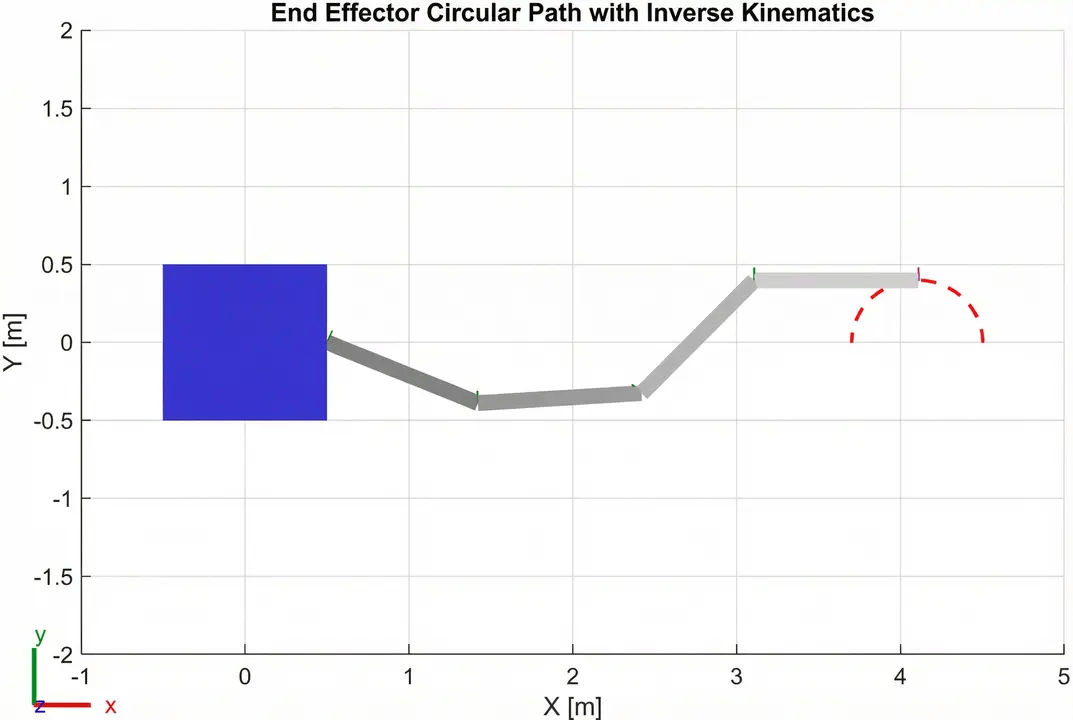
\includegraphics[width=\linewidth]{Figures/ref_kreisbahn_2.png}
    \end{subfigure}
    \vspace{0.5em}
    \begin{subfigure}{0.45\textwidth}
        \centering
        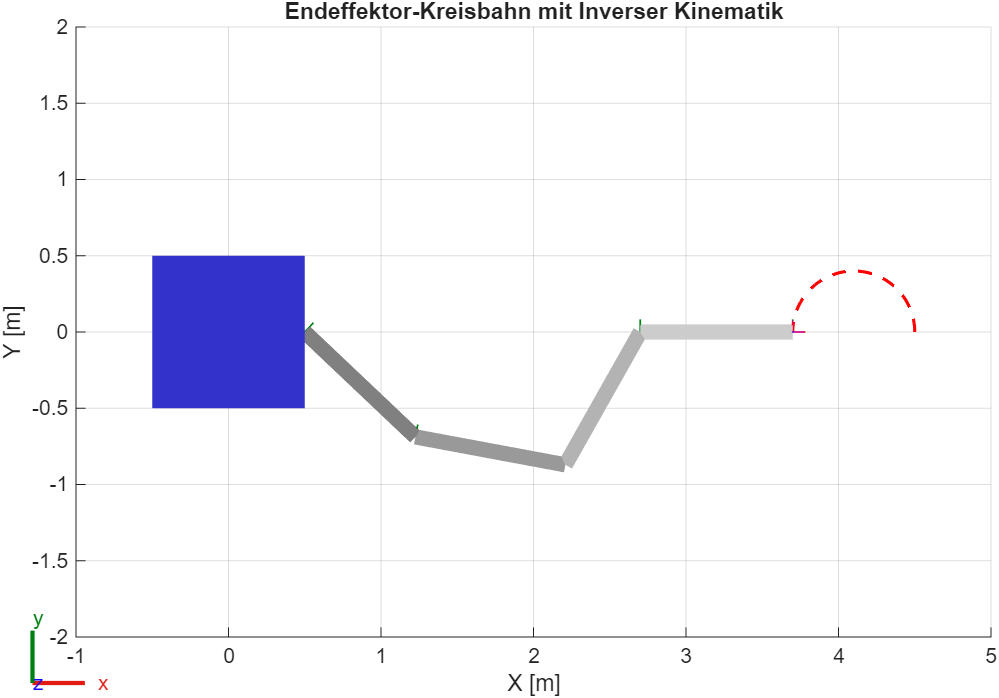
\includegraphics[width=\linewidth]{Figures/ref_kreisbahn_3.png}
    \end{subfigure}
    \caption{Tracking the desired end-effector circular path using inverse kinematics.}
    \label{fig:ref_kreis_gesamt}
\end{figure*}
\noindent
\subsection{Advantages of AI-Endowed Digital Twin Technology in On-Orbit Servicing}

Recent advances in AI-driven DTs have demonstrated considerable benefits for on-orbit servicing, ranging from automated lifecycle management of satellites to the orchestration of skillful agents that autonomously carry out complex assembly, integration, and testing tasks \cite{leutert2024ai,muhlbauer2025towards}. By combining contextualized real-time sensor data with AI methods that account for uncertainty, DTs bridge the physical and digital domains and enable simulation-driven analysis under diverse operational conditions at reduced cost. Verification and validation also benefit from this paradigm, as changes in system design or operational scenarios can be described in scenario spaces and integrated with DTs for flexible verification \cite{maqbool2025systems}.

\hl{[R1.1] In this work,  the information model of the DTs associated with the target satellite and the chaser space robot provides a structured and interoperable description of the satellite and robotic systems, including their kinematics, inertial properties, joint configurations, and physical constraints. The AI capability is embodied by a deep reinforcement learning agent, specifically PPO, which is trained and evaluated through interaction with the corresponding DTs and additional DTs involved in representative in-space operation scenarios. This distinguishes the proposed approach from classical simulation: rather than relying on pre-specified controllers, the robotics-related DT hosts a learning-based agent that autonomously synthesizes control strategies from experience. In this way, the DTs are not limited to reproducing predefined system behavior, but serve as adaptive training and validation environments that support the evolution of control strategies under varying operational conditions. During training, scenarios and constraints are sampled from bounded uniform distributions, allowing the agent to explore a broad range of admissible operating conditions. This improves robustness to modeling errors, disturbances, and partially unknown dynamics without requiring explicit model knowledge.}



\begin{figure*}[!t]
	\centering
	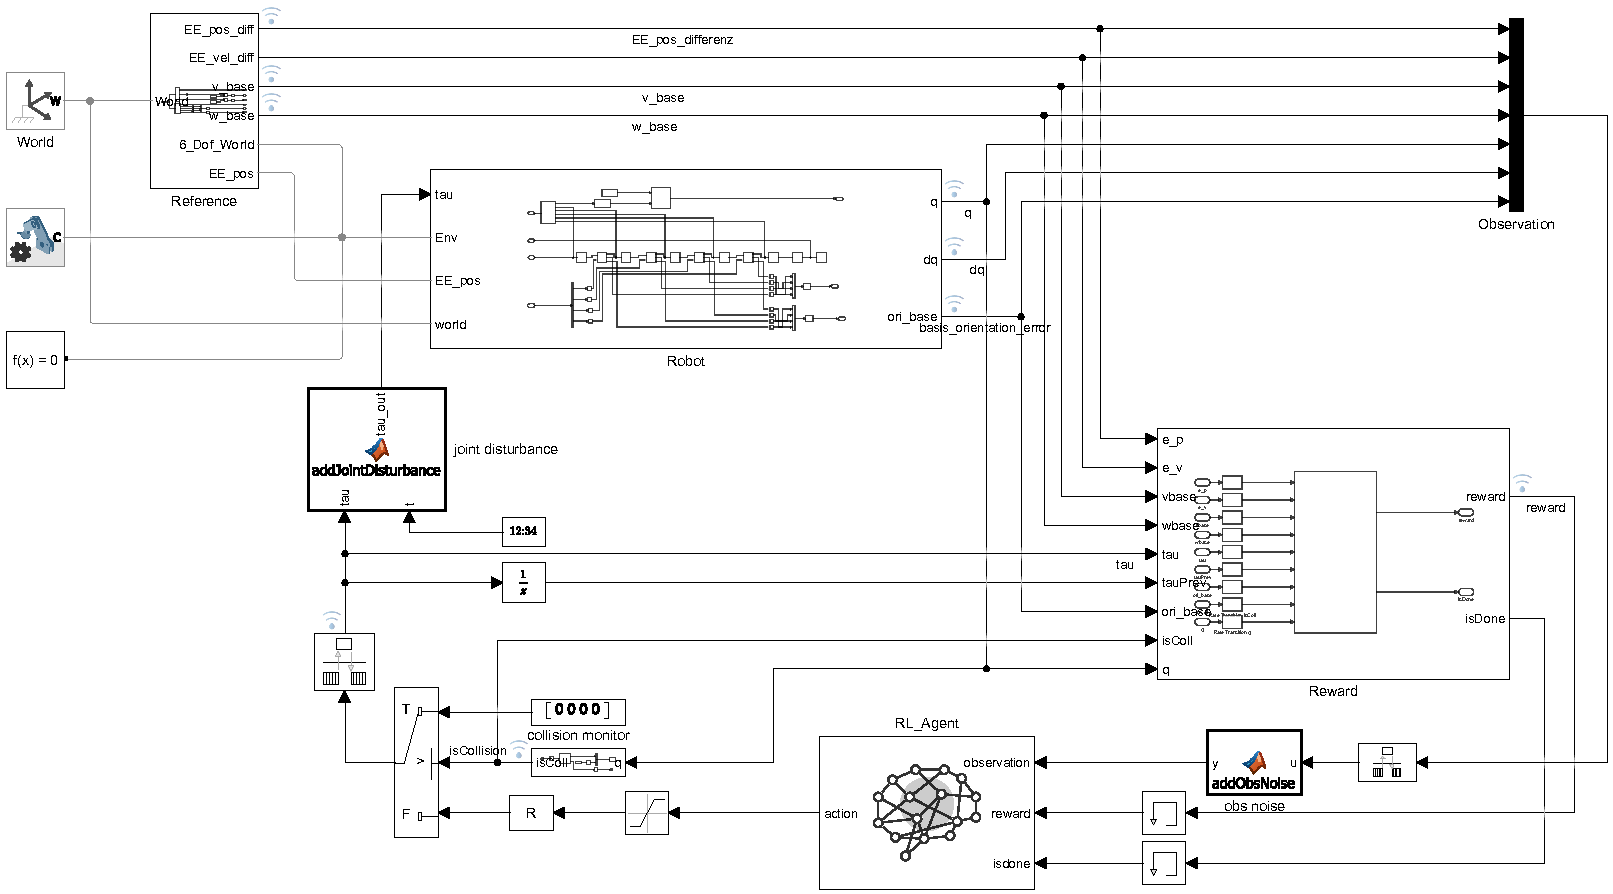
\includegraphics[width=0.98\linewidth]{Figures/Spacerobot_slx.pdf}
	\caption{Overview of the Simulink model \texttt{SpaceRobot.slx} \\
  This figure shows the Simulink-based closed-loop simulation framework for the free-floating space robot. The model integrates the robot dynamics, 
  reference generation, observation assembly, reward computation, and a PPO-based reinforcement learning agent that outputs joint torques. The reward and 
  termination logic evaluate end-effector tracking performance, base motion disturbance, and control effort to guide policy learning.}
	\label{fig:spacerobot_slx}
\end{figure*}

\subsection{Robot Model} The virtual testbed simulates a free-floating space manipulator derived from
the Spacecraft Robotics Toolkit (SPART) example \cite{b9}. The robot consists of a cuboid base (serving as the
spacecraft) and a 4-degree-of-freedom (4-DOF) serial manipulator (see~\autoref{fig:ref_kreis_gesamt}). The arm
has four revolute joints and four links; its kinematic structure and inertial properties are specified in
a Unified Robot Description Format (URDF) file (\texttt{SpaceRobot.urdf}) imported into Simulink's
multibody environment \cite{b25,b26,b27}. The geometry and the inertial properties of the links are taken from identified values reported in the literature (see, e.g., \cite{b12}) and stored in the URDF model. The resulting multibody model captures the dynamic coupling between the floating base and the arm \cite{b6}.

\subsection{Dynamic Simulation in MATLAB/Simulink}\label{sec:sim} The simulation is implemented in Simulink using the
Simscape Multibody physics engine. Gravity is set to $[0~0~0]^T$ to emulate the microgravity
orbital environment. The base is connected to the inertial world frame through an unactuated 6-DoF joint \cite{b3}, allowing free translation and rotation. No external forces or torques act on
the system, so the base moves only in response to the internal torques generated by the manipulator joints. Under this configuration, the total linear and angular momentum are conserved, and arm motions induce a reactive motion of the base \cite{b3,b6,b28,b34,kaigom2011optimal}.

\begin{rthreehl}
\hlthree{[R3.2]} The simulation operates under a set of idealizing assumptions that are standard in RL-based space robotics research and are explicitly acknowledged here to facilitate reproducibility and fair comparison. First, \emph{ideal sensing} is assumed: all state variables (joint angles, joint velocities, base orientation quaternion, and base angular velocity) are read directly from Simulink signal buses without sensor noise, quantization errors, or measurement bias. Second, \emph{zero communication latency} is assumed: the RL agent receives observations and issues torque commands within the same discrete time step, with no transmission delay between sensing and actuation. Third, the robot is modeled as a \emph{rigid multibody system}: flexible link dynamics, joint compliance, and thermal drift are not included. Fourth, \emph{no external disturbances} act on the spacecraft: gravity gradients, atmospheric drag, solar radiation pressure, and residual magnetic torques are all set to zero, consistent with the free-floating assumption in low-Earth orbit. These assumptions establish a clean, controlled benchmark environment in which performance differences can be attributed unambiguously to algorithmic choices rather than to environmental variability. Their impact on real-world deployment is discussed in the Limitations section.
\end{rthreehl}

\begin{rthreehl}
\hlthree{[R3.3]} The choice of MATLAB/Simulink as the simulation backbone was made deliberately in view of the alternatives commonly used in robotics and reinforcement learning research, namely Gazebo~\cite{koenig2004gazebo} and MuJoCo~\cite{todorov2012mujoco}. MuJoCo offers a highly optimized contact and multibody solver and has become a de-facto standard for RL benchmarks in continuous control~\cite{korber2021comparing}; however, it lacks a native interface to Simulink, Stateflow, and the model-based formal verification ecosystem that this work relies on to express and analyze safety monitors. Gazebo provides mature ROS integration, plug-in-based sensor models, and is well suited for hardware-in-the-loop development~\cite{collins2021review}, but its general-purpose multibody back-ends are typically less convenient for free-floating spacecraft scenarios and likewise offer no native path to formal verification artifacts. Simscape Multibody, in contrast, delivers a validated multibody solver for the free-floating base--manipulator coupling and integrates seamlessly with Stateflow and the Simulink Design Verifier used to specify the runtime safety monitors that constitute a central contribution of this work; combined with the Reinforcement Learning Toolbox and a deterministic fixed-step solver, this yields a single, reproducible toolchain from physical model through learned policy to formally checked safety logic. \autoref{tab:sim_comparison} summarizes the trade-off: faster raw simulation throughput in MuJoCo and richer sensor and ROS tooling in Gazebo are exchanged here for tight coupling between the dynamics, the RL agent, and the formal-methods pipeline.
\end{rthreehl}

\begin{table}[!t]
\centering
\renewcommand{\arraystretch}{1.25}
\caption{Comparison of simulation platforms relevant to free-floating space robotics with formal safety monitors.}
\label{tab:sim_comparison}
\begin{tabular}{p{2.4cm}p{1.8cm}p{1.5cm}p{1.5cm}}
\toprule
\textbf{Criterion} & \textbf{MATLAB/ Simulink} & \textbf{Gazebo} & \textbf{MuJoCo} \\
\midrule
Physics engine & Simscape Multibody & ODE, Bullet, DART & MuJoCo (native) \\
Free-floating multibody fidelity & High & Medium & High \\
Formal verification integration & Native (Stateflow, Design Verifier) & None & None \\
RL framework & RL Toolbox & gym-gazebo, ROS bridges & Gymnasium, dm\_control \\
Sensor and ROS integration & Limited (via add-ons) & Extensive & Limited \\
Code generation / HIL path & Mature (Embedded Coder) & Via ROS 2 & Limited \\
Licensing & Commercial & Open source & Open source \\
\bottomrule
\end{tabular}
\end{table}

\begin{figure*}[!t]
	\centering
	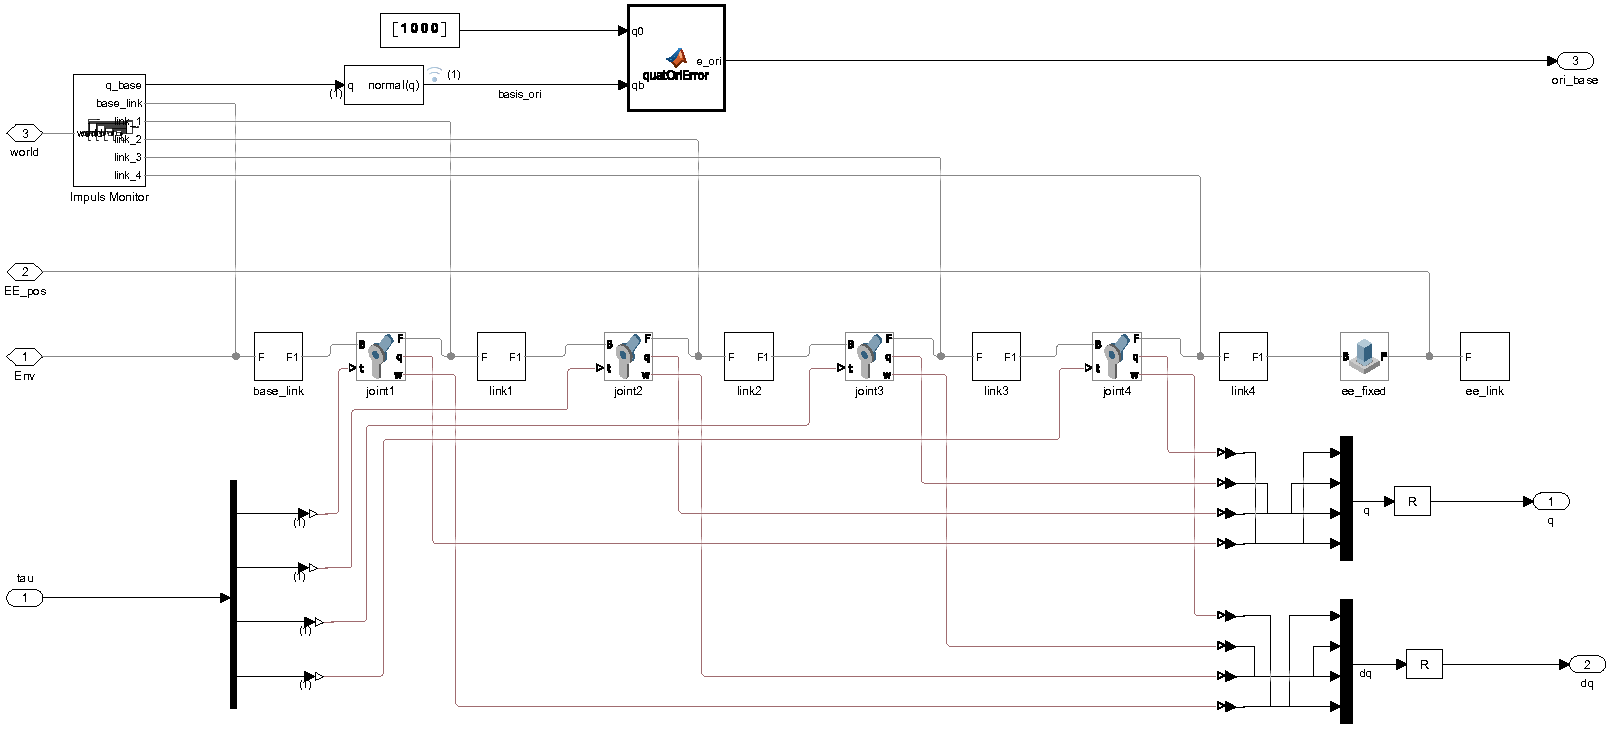
\includegraphics[width=0.98\linewidth]{Figures/spacerobot_slx_robot.pdf}
	\caption{Overview of the Robot Subsystem in the Simulink Model \texttt{SpaceRobot.slx} \\
  This figure depicts the Simulink/Simscape Multibody model of the free-floating space robot, consisting of a floating base 
  and a serial 4-DOF manipulator. Joint torque commands are applied to the revolute joints, while joint positions and velocities 
  are measured and fed back as state variables. The base orientation is represented as a normalized quaternion and compared to a reference to compute the base attitude error.}
	\label{fig:spacerobot_slx_robot}
\end{figure*}

The Simulink model is composed of several subsystems, as illustrated in~\autoref{fig:spacerobot_slx}. The \emph{Robot Plant} subsystem computes
the multibody dynamics of the free-floating robot at each time step (see~\autoref{fig:spacerobot_slx_robot}) by numerically integrating the equations of motion for the applied joint torques~\cite{b6}. The \emph{Controller} subsystem executes the learned RL policy;
the commanded joint torques pass through saturation and safety verification blocks before reaching the plant. When the collision monitor reports an imminent
collision, the controller issues an emergency stop and overrides the torques to zero~\cite{b22,b23}. The \emph{Reference Trajectory Generator} provides the
desired end-effector trajectory and base attitude (see~\autoref{fig:spacerobot_slx_reference}), outputting the current target position and velocity at each time step.
A set of \emph{sensors} measures the robot state (joint angles, joint velocities, base orientation, and base angular velocity) and assembles the observation signal for
the RL agent (detailed in \cref{RL}). Finally, \emph{safety monitors} enforce the operational constraints: a collision monitor compares the distance between selected robot components against a threshold $d_{\mathrm{safe}}$ and triggers a safety halt if the distance falls below this threshold, while a joint-limit monitor triggers an emergency stop if any joint exceeds its admissible range~\cite{b31,b22,b23}.

\begin{figure*}[!t]
	\centering
	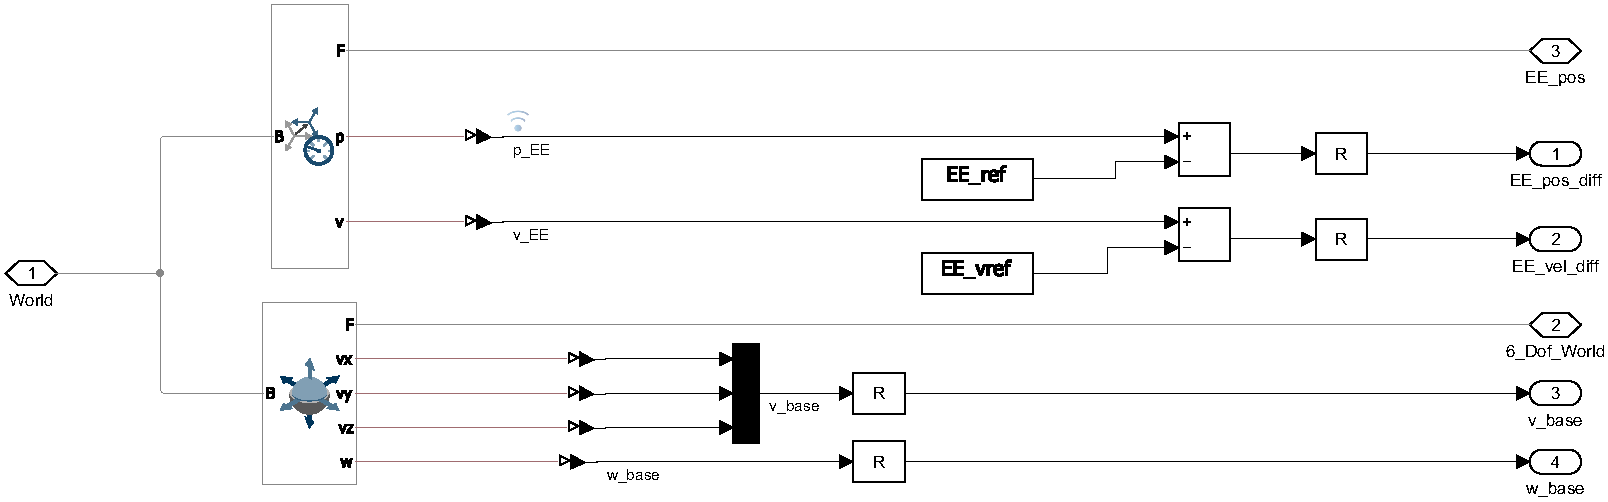
\includegraphics[width=0.97\linewidth]{Figures/spacerobot_slx_reference.pdf}
	\caption{Overview of the Reference Subsystem in the Simulink Model \texttt{SpaceRobot.slx}\\
  This figure shows the computation of end-effector position and velocity tracking errors with respect to the reference trajectory. 
  The measured end-effector states are compared to the reference signals to generate position and velocity error vectors used for observation 
  and reward calculation. In addition, the base linear and angular velocities are extracted to capture base motion induced by manipulator actuation.}            
	\label{fig:spacerobot_slx_reference}
\end{figure*}

To couple the continuous dynamics with the discrete-time RL agent, a
consistent integration scheme is used. The Simscape solver is configured with a fixed-step size
equal to the agent's decision interval ($\Delta t$) instead of the default variable-step solver, ensuring
synchronization between the physics simulation and the RL decision cycle. Rate
transition blocks handle the remaining rate differences and prevent aliasing between the continuous plant and the discrete agent loop \cite{b29,b30}.
Simulink unit consistency checks are enabled to detect modelling errors such as
mismatched units early in development.

\subsection{Reference Trajectory and Desired Task} The task is to follow a periodic end-effector
trajectory while minimizing base disturbance. The reference trajectory is a circular
path (see~\autoref{fig:ref_kreis_gesamt}). Prior to training, the trajectory was validated through inverse kinematics to confirm geometric feasibility for the manipulator (compliance with joint limits and absence of singularities). The inverse-kinematics solution yielded a consistent set of joint trajectories that realize the desired end-effector motion, confirming that the circular path is kinematically feasible.
This precaution ensures that the task is achievable by at least one controller, so that any failure of the RL agent can be attributed to learning, not to a kinematically infeasible reference. During simulation, the reference subsystem outputs the desired end-effector position and velocity
as time series $EE_{\mathrm{ref}}(t)$ and $EE_{v,\mathrm{ref}}(t)$ at each time step. The instantaneous position and velocity tracking errors are derived from these signals; they enter both the observation vector and the reward computation that penalizes large errors.

%The simulation environment provides a flexible and challenging platform for learning, with a free-floating base, a non-trivial trajectory control task, and integrated mechanisms to measure performance and enforce safety. Next, we describe how the reinforcement learning problem is formulated in this environment.

\section{Reinforcement Learning Framework}\label{RL}
\textbf{State (Observation) Space:} At each time step the RL agent receives an observation that summarizes the state variables relevant for control \cite{b7}. The state vector consists of the following components:
\begin{itemize}
  \item \textit{End-effector tracking error:} the Cartesian position error $e_p \in \mathbb{R}^3$ between the current and reference end-effector positions, together with the velocity error $e_v \in \mathbb{R}^3$. When the
end-effector is on the reference trajectory, $e_p = 0$. The pair $(e_p, e_v)$
indicates both the spatial deviation from the reference and the velocity mismatch.
  \item \textit{Arm joint states:} the joint angles $q \in \mathbb{R}^4$ and joint angular velocities $\dot{q} \in \mathbb{R}^4$. These describe the configuration and motion state of the manipulator. Joint angles are provided in radians together with the corresponding mechanical limits.
  \item \textit{Base motion:} the orientation, angular velocity, and linear velocity of the free-floating base. The base attitude error is computed from the measured base quaternion $q_b$ and the reference quaternion $q_0$ as the relative quaternion $q_{\mathrm{err}} = q_0^{*} \otimes q_b$ (with sign convention enforcing a non-negative scalar part), and is then mapped to the axis--angle rotation vector $e_{\mathrm{ori}} = \theta\,\mathbf{u} \in \mathbb{R}^3$, where $\theta = 2\,\mathrm{atan2}(\|q_{\mathrm{err},v}\|,\,q_{\mathrm{err},w})$ and $\mathbf{u} = q_{\mathrm{err},v}/\|q_{\mathrm{err},v}\|$. This 3-dimensional minimal representation removes the redundancy of the unit-quaternion parameterization and is well-defined for $q_{\mathrm{err}} \neq \pm[1,0,0,0]^T$. Since the base is expected to maintain its initial attitude, $e_{\mathrm{ori}}$ is kept near zero through the agent's actions. The base angular velocity $\omega_{\mathrm{base}} \in \mathbb{R}^3$ and the base linear velocity $v_{\mathrm{base}} \in \mathbb{R}^3$ are additionally included to capture residual rotation and momentum-coupled translation of the base.
\end{itemize}

The overall observation vector has dimension $3(e_p) + 3(e_v) + 4(q) + 4(\dot{q}) + 3(\mathrm{ori}_{\mathrm{base}}) + 3(\omega_{\mathrm{base}}) + 3(v_{\mathrm{base}}) = 23$. This state representation contains the variables required by the agent to assess tracking deviation, arm configuration, and base motion.

\textbf{Action Space:} The action is a vector of continuous joint torque commands.
At each decision step, the agent outputs $a = [\tau_{1},\, \tau_{2}, \tau_{3},\, \tau_{4}]^T$, with one component per revolute joint of the arm \cite{b2,b7}. The actions are real-valued and bounded by the actuator capabilities: symmetric torque limits $|\tau_{i}| \leq \tau_{\max}$ for $i = 1,\ldots,4$ are enforced through saturation blocks that clip the commanded torque to the interval $[-\tau_{\max}, +\tau_{\max}]$. The value of $\tau_{\max}$ is selected according to the robot design ($\tau_{\max} = 25\,\mathrm{Nm}$ in this work), provided it is large enough to follow the reference trajectory. The saturation enforces both the actuator limits and an upper bound on the applied torque for safety reasons. The action space is therefore $\mathbb{R}^4$, which is compatible with policy gradient and actor-critic methods.

The policy is a mapping from the 23-dimensional state space to
the 4-dimensional action space, $\pi: s \mapsto a$, parameterized by a neural network whose parameters are adjusted during training to maximize the expected cumulative reward.
The agent issues a new torque command at a fixed interval $\Delta t = 0.1\,\mathrm{s}$, which coincides with the fixed simulation step size to ensure consistency between the discrete agent and the continuous plant.


\noindent
\textbf{Reward Function Design:} The reward signal guides the agent toward accurate trajectory tracking
while minimizing base disturbance and enforcing smooth, bounded control actions.
At each discrete time step $t$, the reward $r_t$ is computed as the sum of a progress term and a proximity bonus, minus a weighted cost function:
\begin{equation}
r_t = \frac{1}{C}\left( r_{\text{prog}} + r_{\text{bonus}} - c_t \right),
\label{eq:reward}
\end{equation}
where $C$ is a normalization constant.

To encourage monotonic convergence toward the reference trajectory, a progress reward is defined based on the reduction of the end-effector position error:
\begin{equation}
r_{\text{prog}} = 
\begin{cases}
k_p \left( d_{t-1} - d_t \right), & d_{t-1} > d_t,\\
0, & \text{otherwise},
\end{cases}
\end{equation}
where $d_t = \|e_p(t)\|$ is the Euclidean end-effector position error and $k_p$ is a scaling factor. The previous distance $d_{t-1}$ is stored persistently across time steps.

A small shaping bonus is added when the end-effector is close to the reference point:
\begin{equation}
r_{\text{bonus}} = k_b \exp\!\left(-\left(\frac{d_t}{\sigma}\right)^2\right),
\end{equation}
which improves local convergence behavior near the desired trajectory.

The instantaneous cost $c_t$ penalizes tracking errors, base motion, and control effort:
\begin{align}
c_t =&\;
W_p \|e_p\|^2
+ W_v \|e_v\|^2
+ W_{\text{ori}} \|e_{\text{ori}}\|^2
+ W_{\omega_b} \|\omega_{\text{base}}\|^2 \nonumber \\
&+ W_{v_b} \|v_{\text{base}}\|^2
+ W_u \|\tau\|^2
+ W_d \|\tau - \tau_{t-1}\|^2 ,
\end{align}
where $e_p$ and $e_v$ denote the end-effector position and velocity errors, $e_{\text{ori}}$ the base orientation error, $v_{\text{base}}$ and $\omega_{\text{base}}$ the linear 
and angular base velocities, and $\tau$ the joint torque vector. The final term penalizes changes in control input to promote smooth actuation.

The weights used in all experiments are summarized in~\autoref{tab:reward_weights}.
\begin{rtwohl}
\hltwo{[R2.4]} The physical intuition behind the weight choices is as follows.
The end-effector position error weight $W_p = 150$ is large because trajectory tracking is the primary task objective; a high weight makes the position error the dominant term of the cost at typical error magnitudes.
The velocity error weight $W_v = 25$ is lower than $W_p$ to avoid over-penalizing transient dynamics during fast arm motion, while still discouraging persistent velocity offsets.
The base orientation weight $W_{\text{ori}} = 200$ is the largest in the cost function, reflecting that base attitude disturbance is safety-critical in on-orbit operations: any uncontrolled rotation of the spacecraft base can jeopardize mission success independently of tracking performance.
The base angular velocity weight $W_{\omega_b} = 8$ provides a damping-like penalty on ongoing base rotation, while the linear velocity weight $W_{v_b} = 2$ is kept small because, in a free-floating system initialized with zero total linear momentum, base translation is momentum-coupled to the manipulator motion and is expected to remain limited for the considered task configuration. Recall that manipulator motion can induce base translation because the total system center of mass is conserved. The torque magnitude weight $W_u = 0.02$ and torque-rate weight $W_d = 0.06$ are intentionally small to leave the agent sufficient freedom to explore diverse control actions; the torque-rate penalty is slightly larger to specifically discourage high-frequency chattering in the control signal.
The progress scaling factor $k_p = 10$ is chosen so that the progress reward is of comparable magnitude to the cost terms at typical error levels, preventing it from being dominated.
The proximity bonus parameters $k_b = 0.05$ and $\sigma = 0.02$ are small by design: they provide a weak local guidance signal near the trajectory without creating a strong local attractor that could trap the policy.
Finally, the normalization constant $C = 500$ scales the total reward to a range of approximately $[-1,\, 0]$ under typical operating conditions, which stabilizes value function learning across all tested algorithms.
\end{rtwohl}

\begin{rtwohl}
\hltwo{[R2.7]} At each step, all inputs to the reward function are checked for numerical validity. If any NaN or Inf values are detected, or if the end-effector error exceeds a predefined bound, the episode is immediately terminated and a terminal penalty of $r_{\text{fail}} = -1$ is assigned. This value is matched to the reward scale: with the normalization constant $C = 500$, typical step rewards lie approximately in $[-1,\,0]$, so $r_{\text{fail}} = -1$ corresponds to the lower end of the one-step reward range. The penalty is therefore large enough to discourage invalid states without dominating the cumulative return over an entire episode. A much smaller penalty (e.g., $-0.1$) would provide a weak failure signal, whereas a much larger penalty (e.g., $-100$) could overshadow the remaining reward terms and destabilize value-function learning. Anchoring the failure penalty to the step-reward scale yields a balanced failure signal for policy optimization.
\end{rtwohl}
All reward components were implemented in a MATLAB Function block within the Simulink environment.

\begin{table}[!b]
\centering
\caption{Reward function weights used in all experiments.}
\label{tab:reward_weights}
\begin{tabular}{lcc}
\toprule
\textbf{Term} & \textbf{Symbol} & \textbf{Value} \\
\midrule
End-effector position error      & $W_p$              & 150   \\
End-effector velocity error      & $W_v$              & 25    \\
Base orientation error           & $W_{\text{ori}}$   & 200   \\
Base angular velocity            & $W_{\omega_b}$     & 8     \\
Base linear velocity             & $W_{v_b}$          & 2     \\
Joint torque magnitude           & $W_u$              & 0.02  \\
Torque rate (smoothness)         & $W_d$              & 0.06  \\
Progress scaling factor          & $k_p$              & 10    \\
Proximity bonus scaling          & $k_b$              & 0.05  \\
Proximity width                  & $\sigma$           & 0.02  \\
Reward normalization constant    & $C$                & 500   \\
\bottomrule
\end{tabular}
\end{table}

\textbf{Training Procedure:} An episodic training scheme is used. Each episode corresponds to a
simulation of fixed duration --- either a horizon of $H$ seconds or a fixed number of time steps $N$ --- chosen such that
one episode covers one or two laps of the circular reference. At the start of each episode, the system is reset to an admissible initial condition by a
custom reset function: the initial joint angles are set to a feasible configuration close to the start of the trajectory and the base is set to a defined attitude (the home orientation, at rest). All state variables, integrator states, and logging signals are reset, and the initial state is verified to lie within the safe set (no collisions or limit violations at $t = 0$). The reset function supports randomization of the starting joint angles and the trajectory phase to improve generalization; in this study a fixed start pose is used, with the end-effector placed at a defined point on the circle \cite{b7}.

Within an episode, the agent receives an observation at each step and outputs a torque action. The
simulation runs until the time horizon $H$ is reached or a terminal condition occurs (task completion or safety violation). An early termination is triggered, for example, when the agent causes a collision before completing the trajectory; the corresponding terminal penalty is applied and the episode ends at that instant.

The training loop is the standard policy gradient procedure provided by MATLAB's Reinforcement Learning Toolbox: after each episode (or after a fixed number of steps) the collected state, action, and reward trajectories are used to
update the policy (and the value function, where applicable) according to the chosen RL algorithm \cite{b4}. The algorithm-specific update rules of PPO, DDPG, and the remaining methods are handled by their respective toolbox implementations; this work supplies the experience and the reward signal \cite{b7}.
All agents are trained for the same number of episodes, $N_{\mathrm{train}} = 1000$, which is sufficient for most algorithms to
converge or reach a performance plateau. During training the cumulative episode reward, the mean end-effector tracking error, and the mean base motion are recorded per episode. A successful training run is characterized by an episode return that increases toward zero (negative costs are used) and by a decrease of the tracking error and base motion over time. The number of episodes terminated prematurely by the safety monitors is also tracked and expected to decrease to zero as training progresses.

\begin{rtwohl}
\hltwo{[R2.8]} To ensure reproducibility, all training runs were initialized using MATLAB's Mersenne Twister random number generator with a fixed seed of zero (\texttt{rng(0,`twister')}), applied prior to each training session. For each of the six algorithms, \textbf{three independent training runs} were performed under identical conditions---same environment, reward function, episode length, and initial state---resulting in 18 training runs in total. The policy selection procedure was as follows: after all three runs per algorithm completed, the policy checkpoint achieving the highest mean episodic reward over the final 50 training episodes was identified. This checkpoint was then used exclusively for all subsequent evaluation experiments. The results were relatively consistent across runs for the more stable algorithms (PPO, TRPO), whereas some runs of the less stable methods (e.g.\ DDPG) diverged, which underlines the importance of algorithmic stability in this setting.
\end{rtwohl}

\textbf{Evaluation and Metrics:} After training, each agent's performance was evaluated on $N_{eval}
= 30$ independent episodes from a fixed initial configuration. Over these
evaluation runs, a set of Key Performance Indicators (KPIs) was computed to compare the
agents quantitatively.

\begin{rthreehl}
\hlthree{[R3.10]} The nine KPIs are organized into three groups to aid interpretation: \emph{tracking accuracy} (K2, K3 measure how closely the end-effector follows the reference path), \emph{base stability and safety} (K4 measures spacecraft attitude drift; K5 and K6 capture constraint violations), and \emph{efficiency} (K7 quantifies control smoothness; K8 measures residual base rotation; K9 measures energy consumption). K1 serves as an overall scalar summary of the agent’s performance across all objectives, since it is the cumulative reward that jointly penalizes all undesired behaviors.
\end{rthreehl}

\begin{itemize}
  \item \textbf{K1} --- \emph{Average Episodic Return}: mean cumulative reward per episode; higher is better and reflects overall task success.
  \begin{equation*}
  R_i=\sum_{k=1}^{T_i} r_i[k], \qquad K1=\frac{1}{N_{\text{eval}}}\sum_{i=1}^{N_{\text{eval}}} R_i.
  \end{equation*}

  \item \textbf{K2} --- \emph{Mean Squared EE Position Error}: average squared tracking error per episode; lower is better.
  \begin{equation*}
  K2=\frac{1}{N_{\text{eval}}}\sum_{i=1}^{N_{\text{eval}}}\frac{1}{T_i}\sum_{k=1}^{T_i}\|e_{p,i}[k]\|_2^2.
  \end{equation*}

  \item \textbf{K3} --- \emph{Maximum EE Position Error}: worst-case tracking deviation; lower is better.
  \begin{equation*}
  K3=\max_{i}\max_{k}\|e_{p,i}[k]\|_2.
  \end{equation*}

  \item \textbf{K4} --- \emph{Mean Base Orientation Error}: average attitude drift of the spacecraft base, measured as the magnitude of the axis--angle rotation-vector error $e_{\mathrm{ori}}$ (in radians); lower is better.
  \begin{equation*}
  K4=\frac{1}{N_{\text{eval}}}\sum_{i=1}^{N_{\text{eval}}}\frac{1}{T_i}\sum_{k=1}^{T_i}\|e_{\mathrm{ori},i}[k]\|_2.
  \end{equation*}

  \item \textbf{K5} --- \emph{Collision Rate}: fraction of episodes with at least one collision; zero is ideal.
  \begin{equation*}
  C_i=\mathbb{I}(\exists k:\,c_i[k]>0.5), \qquad K5=\frac{1}{N_{\text{eval}}}\sum_{i=1}^{N_{\text{eval}}} C_i.
  \end{equation*}

  \item \textbf{K6} --- \emph{Joint Limit Violation Rate}: fraction of time steps across episodes where any joint exceeds its mechanical limit; zero is ideal.
  \begin{equation*}
  K6=\frac{1}{N_{\text{eval}}}\sum_{i=1}^{N_{\text{eval}}}\frac{1}{T_i n_J}\sum_{k=1}^{T_i}\sum_{j=1}^{n_J}
  \mathbb{I}\!\big(q_{i,j}[k]\notin[q_j^{\min},q_j^{\max}]\big).
  \end{equation*}

  \item \textbf{K7} --- \emph{Control Smoothness (Jerk)}: second difference of joint torques; lower values indicate smoother, less chattering actuation.
  \begin{equation*}
  \begin{aligned}
  \Delta^2\tau_i[k] &= \tau_i[k+2]-2\tau_i[k+1]+\tau_i[k],\\
  J_i &= \frac{1}{T_i-2}\sum_{k=1}^{T_i-2}\|\Delta^2\tau_i[k]\|_2,\\
  K7 &= \frac{1}{N_{\text{eval}}}\sum_{i=1}^{N_{\text{eval}}}J_i.
  \end{aligned}
  \end{equation*}

  \item \textbf{K8} --- \emph{Mean Base Angular Velocity}: residual spacecraft rotation rate during the task (rad/s); lower is better, ideally zero.
  \begin{equation*}
  K8=\frac{1}{N_{\text{eval}}}\sum_{i=1}^{N_{\text{eval}}}\frac{1}{T_i}\sum_{k=1}^{T_i}\|\omega_{b,i}[k]\|_2.
  \end{equation*}

  \item \textbf{K9} --- \emph{Energy Consumption}: average absolute mechanical power integrated over each episode; lower is better when not at the expense of tracking quality.
  \begin{equation*}
  E_i=\int\sum_{j=1}^{n_J}\big|\tau_{i,j}(t)\,\dot q_{i,j}(t)\big|\,dt, \qquad
  K9=\frac{1}{N_{\text{eval}}}\sum_{i=1}^{N_{\text{eval}}} E_i.
  \end{equation*}
\end{itemize}


\begin{rthreehl}
\hlthree{[R3.6]} Two KPIs deserve explicit justification in the space mission context. \textbf{K7 (Control Smoothness)} captures high-frequency torque oscillations (chattering): in space, such oscillations can accelerate actuator wear, excite structural vibrations that degrade the pointing accuracy of sensitive instruments such as cameras or star trackers, and dissipate energy through rapid back-and-forth motion. Minimizing K7 therefore supports hardware lifetime and payload pointing requirements. \textbf{K9 (Energy Consumption)} reflects the mechanical work performed by the joints, approximated as $\int |\tau \cdot \dot{q}|\,dt$. Onboard power is limited by solar panel area and battery capacity; energy spent on control actuation reduces the budget available for communication, thermal management, and payload operation. Reducing K9 without sacrificing tracking accuracy therefore has operational value for mission planning.
\end{rthreehl}

In addition to the KPIs above, three training-related metrics are reported: T1, the variance of the episodic reward in the late stage of training (an indicator of training stability); T2, the variance of the value function or average reward (a second stability metric); and T3, the wall-clock training time required for 1000 episodes (an indicator of sample efficiency and computational load).

Applying these metrics to all six agents yields a common basis for comparison. The comparative results are presented and discussed in \Cref{comparison}.

\section{Safety Monitoring and Constraint Enforcement}\label{formal}
Stability and safety are central requirements in space robotics. A controller for autonomous on-orbit servicing must satisfy the physical constraints of the system and avoid hazardous states, in particular when the control policy is learned from data and must therefore handle uncertainty. In this work, runtime safety monitors and constraint-enforcement mechanisms are integrated directly into the RL training and execution environment. They serve two purposes: protecting the simulation from unsafe states during exploration, and shaping the agent's behaviour toward safe operation through penalty-driven learning~\cite{b7,b22}.

\begin{figure*}[!t]
\centering
   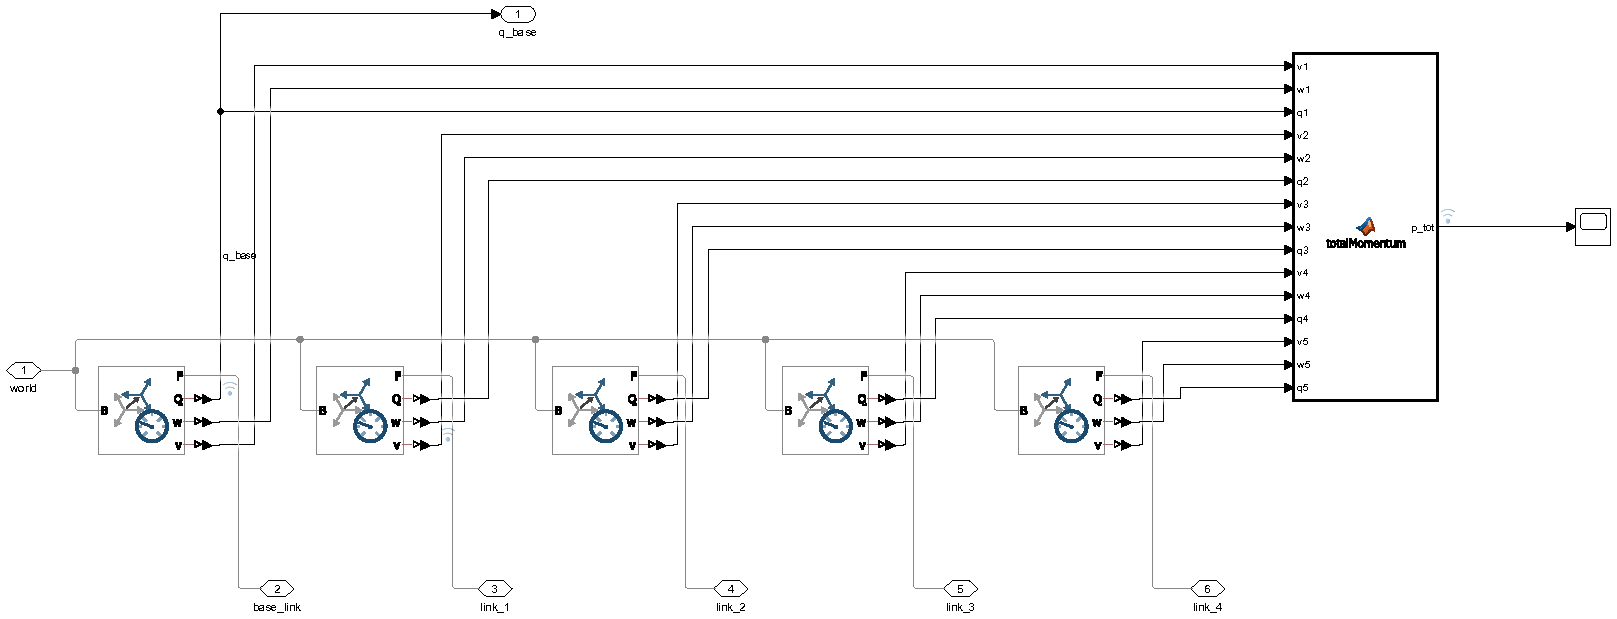
\includegraphics[width=1\linewidth]{Figures/impuls_monitor.pdf}
    \caption{Overview of the Momentum Monitor Subsystem (Momentum Observer) in the Simulink Model \texttt{SpaceRobot.slx} \\
    This figure shows the computation of the total linear and angular momentum of the free-floating space robot. 
    The velocities and orientations of the base and all manipulator links are measured and aggregated within a 
    MATLAB function to obtain the system momentum. This monitor is used to analyze momentum conservation and 
    quantify base–manipulator dynamic coupling effects.}
    \label{fig:impuls_monitor}
\end{figure*}
\begin{figure}[!b]
  \centering
  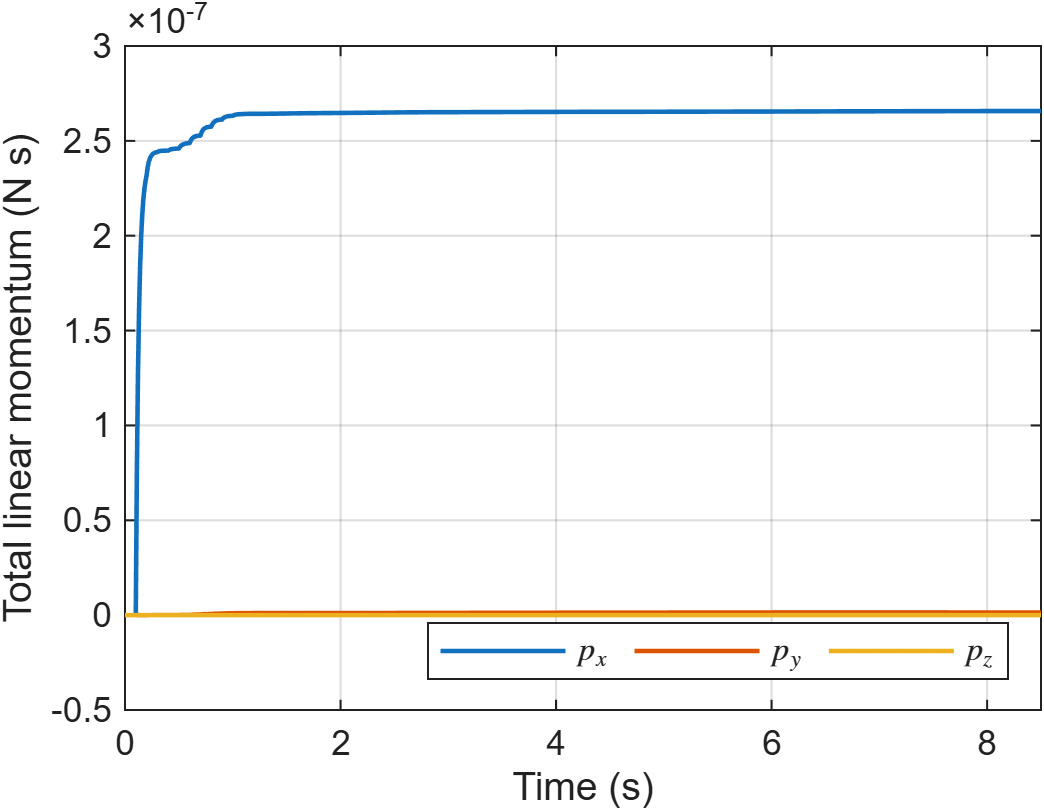
\includegraphics[width=0.95\linewidth]{Figures/impulserhaltung_scope.png}
  \caption{Dynamics of the total momentum of the robot.}
  \label{fig:impulserhaltung_scope}
\end{figure}
\noindent
\textbf{Momentum Conservation Monitor.} In a free-floating system without external forces, the total linear momentum of the robot (base and arm) is conserved; with zero initial momentum, it remains close to zero throughout the simulation \cite{b6}. A momentum observer continuously
computes the total linear momentum $p_{\mathrm{tot}}$ and checks for its conservation (see \Cref{fig:impuls_monitor}). Virtual sensors attached to the base and to each link provide the body velocities, from which $p_{\mathrm{tot}} = \sum_{i} m_{i} v_{i}$ is computed. In an ideal simulation, $p_{\mathrm{tot}}$ remains close to zero throughout an episode; small numerical deviations on the order of $10^{-6}\,\mathrm{Ns}$ may arise from time-integration errors. A persistent, systematic drift of $p_{\mathrm{tot}}$ would indicate an unintended external force or a modelling error, such as an unmodelled constraint. In the reported experiments, $p_{\mathrm{tot}}$ remained within $10^{-6}\,\mathrm{Ns}$ of zero throughout each episode with the learned policy (see~\autoref{fig:impulserhaltung_scope}), which confirms the physical consistency of the simulation. The momentum observer also serves as a diagnostic tool, as any momentum drift would pause training for model inspection.

\begin{figure*}[!t]
    \centering    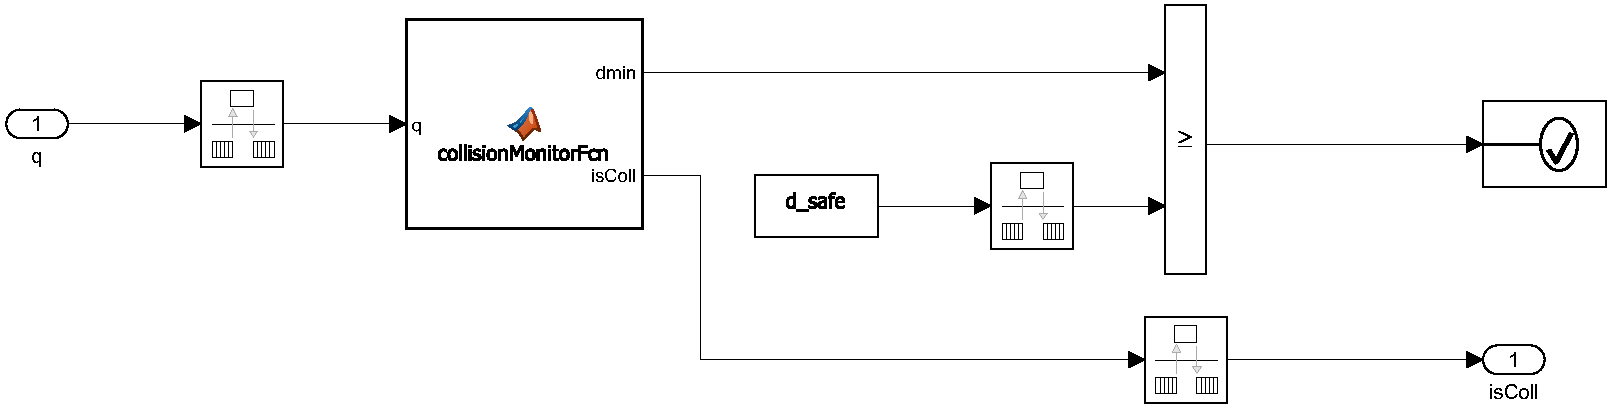
\includegraphics[width=0.75\linewidth]{Figures/spacerobot_slx_colissionmonitor.pdf}
    \caption{Overview of the Collision Monitor Subsystem in the Simulink Model \texttt{SpaceRobot.slx} \\
    This figure illustrates the collision monitoring logic used to ensure safe robot operation during training and 
    evaluation. Joint and link configurations are processed to compute the minimum distance to obstacles, which is 
    compared against a predefined safety threshold. A collision flag is generated and used for episode termination 
    or safety-related penalties.}
    \label{fig:spacerobot_slx_colissionmonitor}
\end{figure*}

\begin{figure*}[!t] 
    \centering
    \begin{subfigure}[b]{0.48\textwidth}
        \centering
        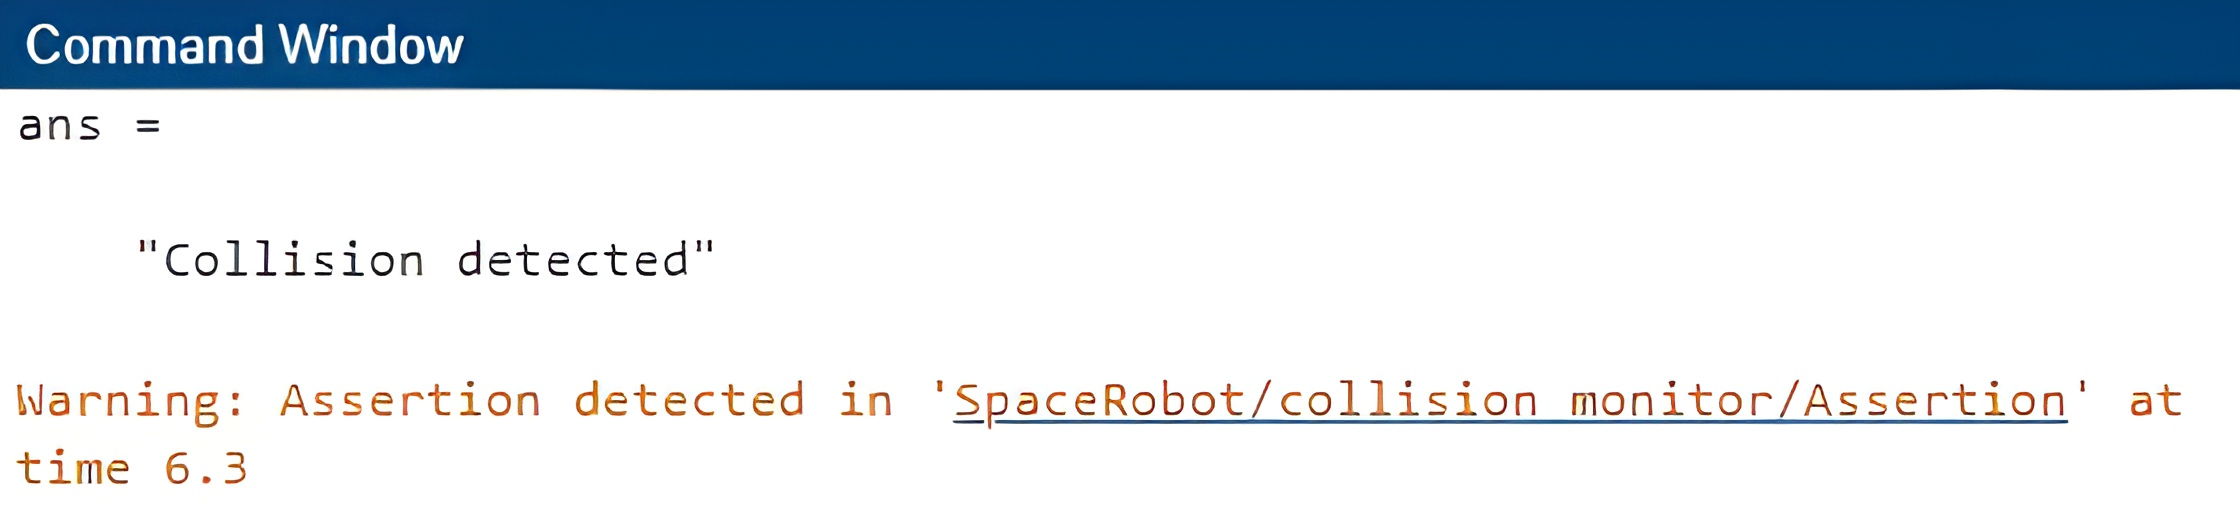
\includegraphics[width=\linewidth]{Figures/warning_collision.png}
        \caption{Automatically triggered collision warning}
        \label{fig:collision_warning}
    \end{subfigure}
    \hfill
    \begin{subfigure}[b]{0.48\textwidth}
        \centering
        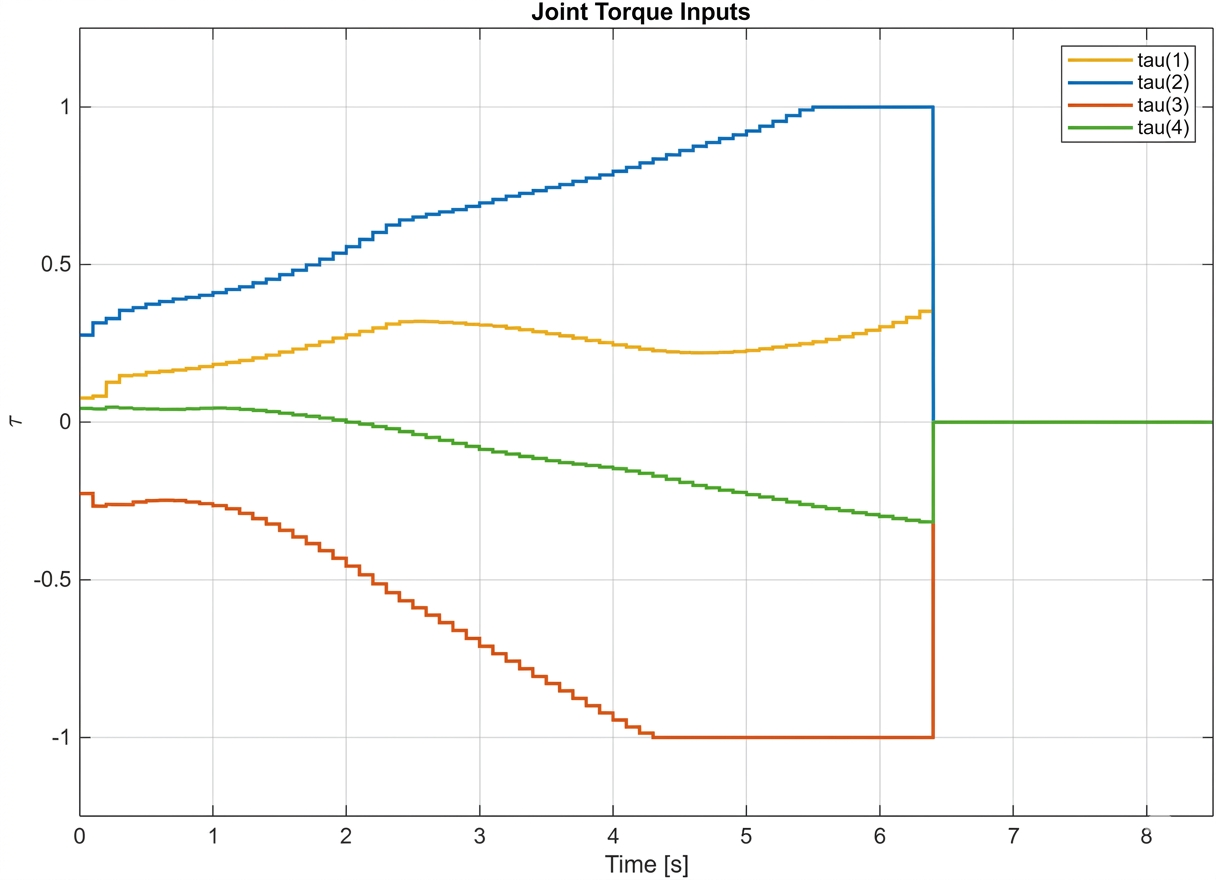
\includegraphics[width=\linewidth]{Figures/tau_collision.png}
        \caption{Scope of torque inputs in the event of a collision}
        \label{fig:collision_scope}
    \end{subfigure}
    \caption{Representation of collision detection and the associated torque curves.}
    \label{fig:collision_combined}
\end{figure*}
\noindent
\textbf{Collision Monitor and Avoidance.} A minimum admissible distance is defined between selected
parts of the robot (e.g.\ between the end-effector and the base structure). At every time step, a collision monitor computes the distances between the predefined body pairs using the URDF geometry and the Simscape collision-detection facilities. When any distance drops below the safety threshold $d_{\mathrm{safe}}$, a collision event is triggered (see \Cref{fig:spacerobot_slx_colissionmonitor}) \cite{b31}. A value of $d_{\mathrm{safe}} = 5\,\mathrm{cm}$ is used in this work. Upon activation, three actions are performed: (i)~a warning flag is raised and logged, (ii)~a \texttt{done} signal terminates the episode, and (iii)~all commanded joint torques are overridden to zero, stopping the robot. The monitor was verified by intentionally commanding the arm toward the base; it reliably detected the threshold violation and stopped the system (see~\autoref{fig:collision_combined}). During training, collisions occurred in early exploratory
episodes for some agents, but were captured by the monitor and penalized through episode termination. By the end of training, all agents avoided collisions in the final evaluation ($K_5 = 0$ over all 30 evaluation episodes).

\textbf{Joint Limit Enforcement.} Each revolute joint of the arm is subject to mechanical limits. Violating these limits could damage a real robot and typically indicates an unstable controller. The joint limits are enforced at two levels. First, the Simscape model includes mechanical joint limits with penalty forces, i.e.\ a stiff barrier that opposes further motion beyond the limit. Second, an assertion block monitors each joint angle; if any joint exceeds its admissible range, the assertion triggers a violation event that terminates the episode, applies a negative terminal reward, and sets all torques to zero within the same time step. This prevents further motion into the limit. After training, the joint-limit violation rate is low: PPO and TRPO reach the limits in a few percent of evaluation steps (5.1\% and 2.1\%, respectively), whereas TD3, SAC, PG, and DDPG remain within the admissible range ($K_6 \approx 0$). The higher $K_6$ value of PPO ($K_6 = 0.0505$) coincides with the lowest tracking error and indicates a more aggressive use of the workspace. In all cases, the enforcement mechanism stopped further simulated motion at the limit: the torques were set to zero in the offending step and the episode was marked as failed. For the optimized PPO agent (\autoref{sec:reward_ablation}), no such events are observed in the evaluation episodes ($K_6 = 0$).

\textbf{Formal Verification of Torque Constraints.} In addition to runtime saturation, an offline formal verification was performed to check torque-bound compliance of the trained policy block. Using MATLAB Simulink Design Verifier (SLDV) in property-proving mode,
a simplified closed-loop model of the agent and the joint torques was analyzed. The property to be checked is that, for any admissible observation input in the analyzed abstraction, each commanded torque $\tau_i$ satisfies $\tau_i \in [-\tau_{\max}, +\tau_{\max}]$ (see \Cref{fig:verify_tau}). SLDV found no counterexample for this property; the corresponding SLDV result is shown in \autoref{fig:verify_tau_result} \cite{b5}. This result applies to the simplified verification model, including admissible abstract states not visited during simulation. Note that the full Simscape model is not amenable to property proving because of the nonlinear dynamics; the verification was performed on a simplified model (\texttt{Verify\_tau.slx}) in which the plant was replaced by a worst-case abstraction, because only the policy output block is relevant for the considered property. This illustrates how formal methods can complement simulation-based learning by checking selected properties on an abstracted model of the agent.

\begin{figure}[!b]
	\centering    
	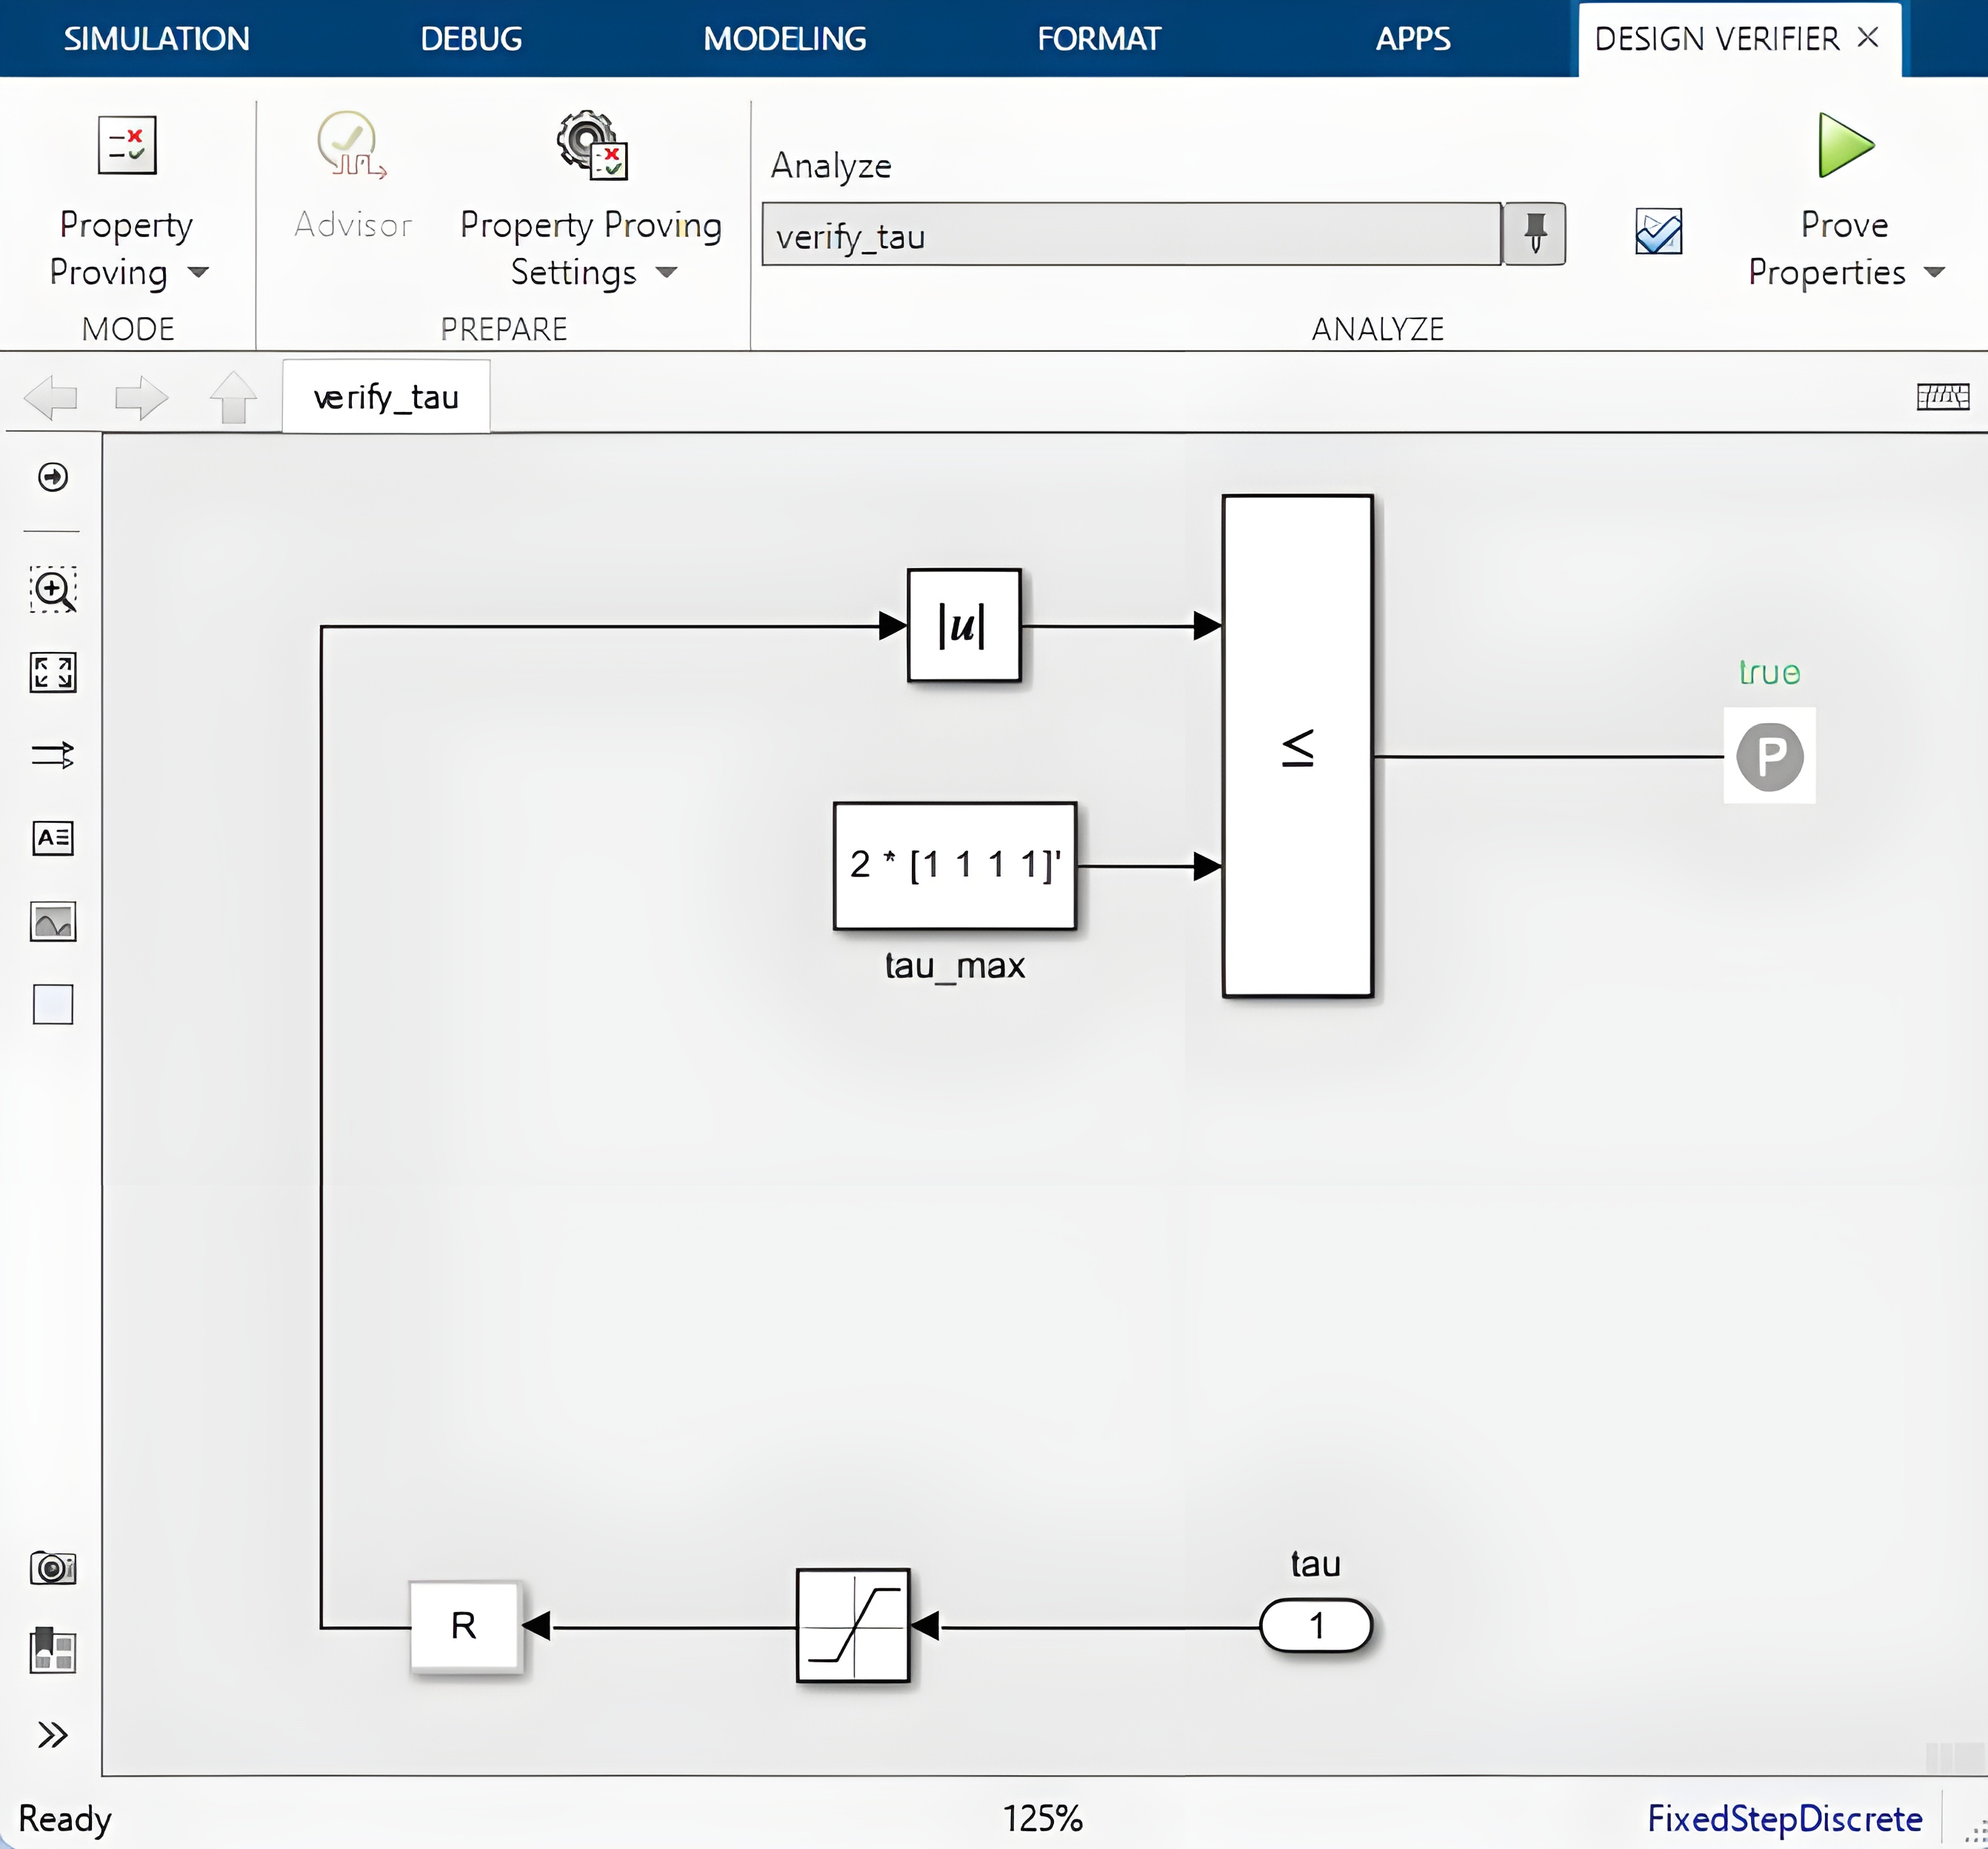
\includegraphics[width=\linewidth]{Figures/verify_tau_slx.png}
	\caption{Verification model with Simulink Design Verifier \texttt{Verify\_tau.slx} \\
  This figure depicts the Simulink property model used to formally verify the joint torque constraints. 
  The absolute joint torques are compared against predefined maximum limits using a relational operator. 
  The property is checked over the analyzed abstract state space, supporting bounded control actions in the verification model.}
	\label{fig:verify_tau}
\end{figure}

\textbf{Limitations of the Formal Methods Component.} The mechanisms above cover a defined set of monitored properties: collision events, joint-limit events, bounded torques, and physical consistency through the momentum check. Other properties, such as task completion within a time bound or formal stability margins, are not verified. A complete formal specification of the mission --- for example, temporal-logic specifications such as ``the robot shall accomplish $X$ without $Y$ happening'' --- would be substantially more complex. The present work targets the safety properties that are most relevant for the considered task. Within this scope, the runtime monitors terminated episodes that would have violated a monitored property and penalized the corresponding actions. By the end of training, the policy operated within the safety envelope defined by the monitored constraints in the reported evaluation episodes \cite{b23}.

In summary, the formal safety checks integrated into the learning process helped prevent unsafe simulated states during the exploratory phase of training and shaped the agent's behaviour by penalizing unsafe actions. The agent therefore learns with a runtime safety shield. This combination of monitored runtime constraints and penalty-driven learning is one approach to deploying deep RL in safety-critical domains such as space robotics, in which unconstrained trial-and-error exploration is not admissible. The next section analyses the performance of the six RL agents under these conditions.

\begin{rthreehl}
\hlthree{[R3.5]} \textbf{Computational Overhead and Scalability:} The three safety monitors --- momentum observer, collision distance checker, and joint-limit assertion --- each consist of simple algebraic operations over the robot's link states, scaling as $\mathcal{O}(n_{\text{links}})$ per time step. For the 4-DOF arm considered here, this overhead is negligible compared to the physics simulation itself. End-to-end training times, including the full safety stack, are reported as metric T3 in \autoref{tab:kpi_comp}: they range from approximately 8 minutes (PG, PPO) to 38 minutes (TD3) for 1000 episodes on a standard workstation (AMD Ryzen 7 7700, 32 GB RAM). For onboard deployment, only the learned policy network needs to execute in the control loop. The default PPO baseline uses a compact two-hidden-layer network (128 units per layer, $\approx$\,20\,000 parameters), while the optimized PPO configuration adopted for the final results (cf.\ \cref{sec:reward_ablation}) uses a deeper $[256, 256, 128]$ policy with $\approx$\,1.05$\,\times\,10^{5}$ parameters --- still on the order of $10^5$ weights and well below the memory footprint of typical perception networks deployed on space-qualified hardware. At the 10\,Hz control rate used here, a single forward pass through this network requires on the order of $2\,\times\,10^{5}$ multiply-accumulate operations per step, which is compatible with the throughput of modern space-qualified embedded processors (e.g., ARM Cortex-A or LEON-class CPUs with a hardware FPU). The safety monitors can be retained as lightweight parallel watchdog processes, or reduced to the most safety-critical checks (torque saturation, joint-limit assertion) with minimal additional compute. This modular architecture supports scalability to resource-constrained onboard systems.
\end{rthreehl}

\begin{figure}[!b]
	\centering
	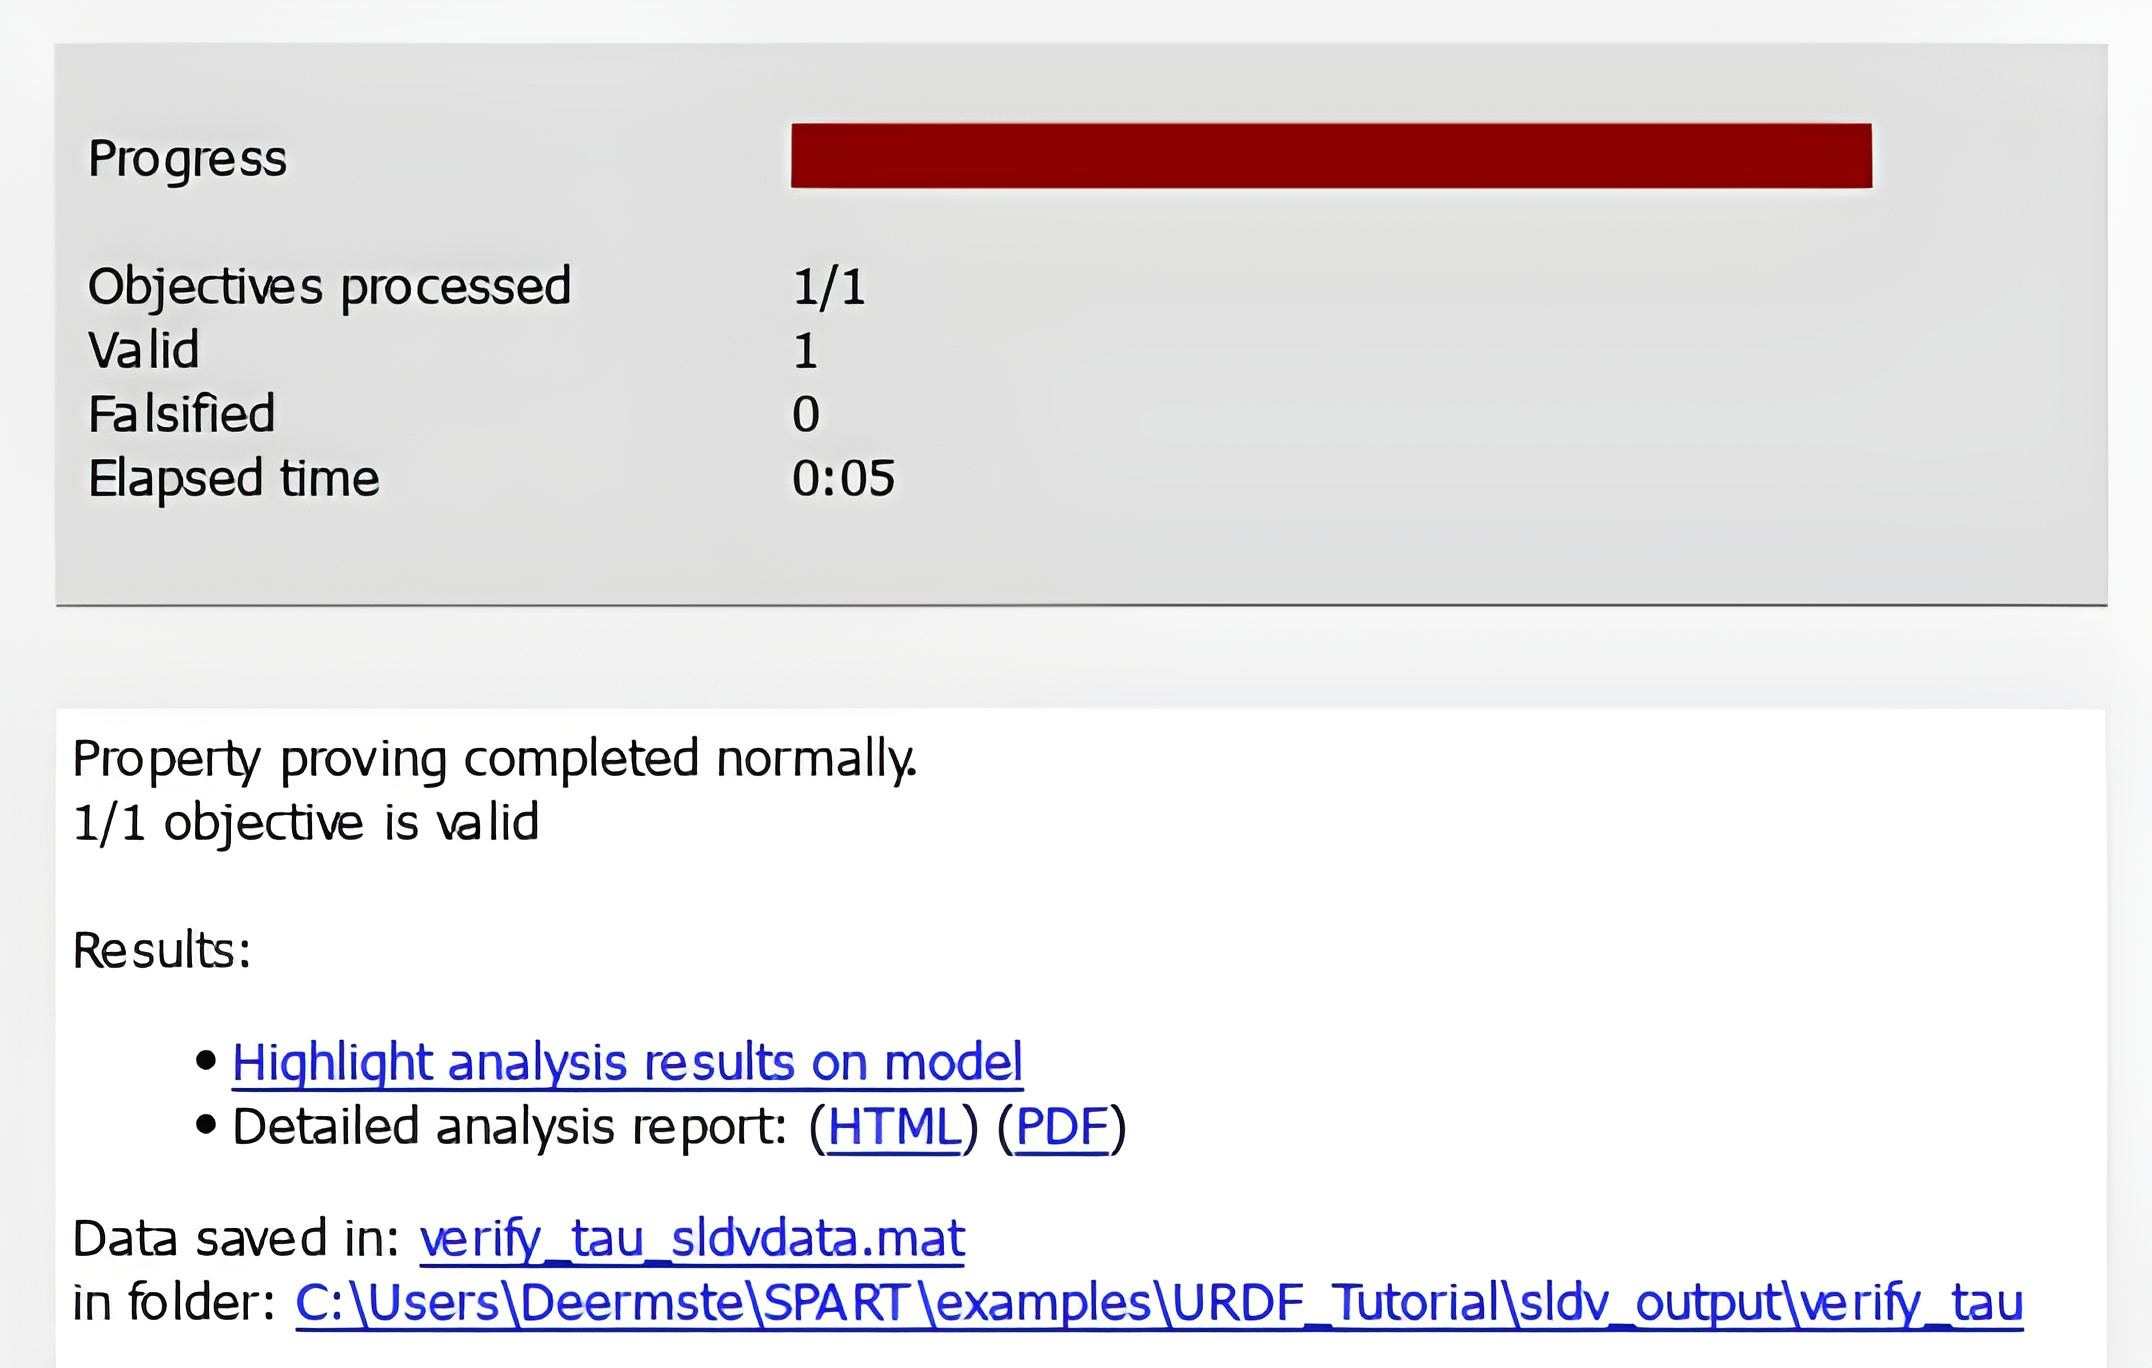
\includegraphics[width=\linewidth]{Figures/verify_tau_reslult.png}
	\caption{Result of the Simulink Design Verifier \\ 
  This figure shows the result of a formal property verification performed on the torque constraint model. 
  The verification confirms that the specified safety property is satisfied for all analyzed execution paths. 
  This analysis provides model-based evidence for torque-limit compliance beyond empirical simulation-based validation.}
	\label{fig:verify_tau_result}
\end{figure}

\section{Comparison of Continuous RL Agents} \label{comparison}
This section compares six continuous-action RL algorithms from three families on the same task and environment \cite{b2,b7}. The algorithms considered are:

\begin{itemize}
  \item \textit{Policy Gradient (PG):} the REINFORCE algorithm (Monte Carlo policy gradient), included as
a baseline for direct policy optimization without variance-reduction techniques \cite{b7,b21}.
  \item \textit{Proximal Policy Optimization (PPO):} a policy-gradient method that uses a clipped
probability-ratio surrogate to bound policy updates \cite{b15}.
  \item \textit{Trust Region Policy Optimization (TRPO):} a policy-gradient method that enforces a trust-region
constraint based on the Kullback--Leibler divergence at each update; the constrained optimization step incurs a higher per-update computational cost than PPO \cite{b14}.
  \item \textit{Deep Deterministic Policy Gradient (DDPG):} an off-policy actor-critic algorithm with a
deterministic policy and target networks; DDPG jointly learns a $Q$-function and a policy and is sensitive to hyperparameter choices \cite{b16}.
  \item \textit{Twin Delayed DDPG (TD3):} a variant of DDPG that uses two critic networks to reduce overestimation bias and delays policy updates relative to value updates \cite{b17}.
  \item \textit{Soft Actor-Critic (SAC):} an off-policy actor-critic algorithm with a stochastic policy and an entropy term in the objective; this entropy regularization promotes exploration but increases the per-step computational cost relative to deterministic methods \cite{b18}.
\end{itemize}

The six algorithms cover the on-policy/off-policy and deterministic/stochastic axes, as well as a range of update rules. Given the strong base--manipulator coupling and the safety constraints, methods with constrained or clipped policy updates (PPO, TRPO) are expected to provide more stable training than algorithms without such constraints (PG, DDPG). The off-policy actor-critic methods (DDPG, TD3, SAC) may achieve comparable performance but are typically more sensitive to hyperparameter selection.

\begin{table}[!t]
\centering
\caption{Classification of the evaluated reinforcement learning algorithms.}
\label{tab:on_off_policy}
\begin{tabular}{ll}
\toprule
\textbf{Algorithm} & \textbf{Policy Type} \\
\midrule
Policy Gradient (PG) & On-policy \\
Proximal Policy Optimization (PPO) & On-policy  \\
Trust Region Policy Optimization (TRPO) & On-policy  \\
Deep Deterministic Policy Gradient (DDPG) & Off-policy  \\
Twin Delayed DDPG (TD3) & Off-policy  \\
Soft Actor-Critic (SAC) & Off-policy  \\
\bottomrule
\end{tabular}
\end{table}
On-policy methods (PG, PPO, TRPO) update the policy only from data generated by the current policy, which typically leads to stable but less sample-efficient learning. Off-policy methods (DDPG, TD3, SAC) reuse experience stored in a replay buffer, which improves sample efficiency at the cost of higher sensitivity to hyperparameters~\cite{b2,b7}. For free-floating space-robot control with strong nonlinear coupling and safety constraints, the constrained-update on-policy methods are expected to provide more reliable convergence.

\textbf{Training Setup.} All experiments were performed on a workstation with an AMD Ryzen 7 7700 processor and 32\,GB of RAM, using MATLAB R2025b with the Reinforcement Learning Toolbox and Simscape Multibody. The same network architecture (two hidden layers of 128 units each for the policy and, where applicable, for the value function) and the same reward function were used for all agents. The discount factor was fixed at $\gamma = 0.99$. The learning rate for both actor and critic networks was $\alpha = 1 \times 10^{-3}$ unless stated otherwise. With these unified settings, observed performance differences can be attributed primarily to the algorithmic differences rather than to unequal tuning. PPO was further tuned in a subsequent step; in the main comparison, PPO uses its default configuration. Each agent was trained for 1000 episodes; the resulting policy was then evaluated.

\textbf{Performance Metrics.} The agents were evaluated on the KPIs introduced in Section~\ref{RL} by running 30 evaluation episodes per agent. \autoref{tab:kpi_comp} reports a subset of these metrics for the six agents.

\begin{table*}[!t]
\centering
\caption{Selected performance metrics for each RL agent (best value in each row in bold). PPO attains the
lowest tracking errors (K2, K3), the lowest base-orientation error (K4), and the lowest jerk (K7), with the
shortest training time (T3). TRPO is close to PPO on several metrics but requires more training time. The
off-policy methods (TD3, SAC, DDPG) show larger errors or a larger late-training reward variance (e.g., high
T1 for DDPG); DDPG attains the lowest maximum error (K3). Values are averaged over 30 evaluation episodes per agent.}
\label{tab:kpi_comp}
\renewcommand{\arraystretch}{1.3}
\setlength{\tabcolsep}{8pt}
\begin{tabular}{lcccccc}
\toprule
\textbf{KPI (unit)} & \textbf{TRPO} & \textbf{TD3} & \textbf{SAC} & \textbf{PPO} & \textbf{PG} & \textbf{DDPG} \\
\midrule
\textbf{K2:} Mean Squared EE position error &
0.0680 & 0.1914 & 0.1908 & \textbf{0.0257} & 0.1638 & 0.0937 \\
\textbf{K3:} Max EE error &
0.6783 & 0.5341 & 0.7766 & 0.4833 & 1.0654 & \textbf{0.4758} \\
\textbf{K4:} Mean base orientation error &
0.0694 & 0.0868 & 0.1687 & \textbf{0.0667} & 0.1302 & 0.2682 \\
\textbf{K6:} Joint limit violation rate &
0.0214 (2.1\%) & 0 & 0 & 0.0505 (5.1\%) & 0 & 0 \\
\textbf{K7:} Torque smoothness (norm.\ jerk) &
0.7498 & 0.9981 & 0.7536 & \textbf{0.6812} & 0.7125 & 0.8118 \\
\textbf{T1:} Reward std.\ (late training) &
\textbf{0.6144} & 8.5168 & 9.6907 & 1.7756 & 13.1970 & 64.4764 \\
\textbf{T3:} Training time (1000 eps) &
$\sim$13\,min & $\sim$38\,min & $\sim$35\,min & \textbf{$\sim$8\,min} & $\sim$8\,min & $\sim$24\,min \\
\bottomrule
\end{tabular}
\end{table*}

The results in \autoref{tab:kpi_comp} display the following patterns. With respect to \emph{training stability}, TRPO and PPO yield the smallest late-training reward variance ($T_1 = 0.61$ and $T_1 = 1.78$, respectively), whereas DDPG shows the largest ($T_1 = 64.5$). The training time $T_3$ is shortest for PPO ($\approx 8\,\mathrm{min}$); the off-policy methods are slower (TD3 $\approx 38\,\mathrm{min}$, SAC $\approx 35\,\mathrm{min}$).

For \emph{trajectory tracking}, PPO attains the lowest mean squared error ($K_2 = 0.0257$), lower than that of TRPO ($K_2 = 0.0680$). DDPG attains the lowest peak error ($K_3 = 0.4758$) but with large variability across runs. PG, SAC, and TD3 yield larger tracking errors; the mean error of PG is approximately six times that of PPO.

For \emph{base-motion minimization}, PPO and TRPO yield comparable base-orientation errors ($K_4 = 0.0667$ and $K_4 = 0.0694$), while DDPG produces a larger drift ($K_4 = 0.2682$). TD3 yields a low base angular velocity ($K_8 \approx 0.02\,\mathrm{rad/s}$) at the cost of degraded tracking accuracy, consistent with a conservative policy that suppresses actuation. All agents avoid collisions ($K_5 = 0$). PPO and TRPO approach the joint limits in a small fraction of the steps ($K_6 = 5.1\%$ and $K_6 = 2.1\%$, respectively), corresponding to a wider use of the joint range.

PPO produces the smoothest control signals ($K_7 = 0.6812$); the highest jerk values are observed for TD3 and DDPG ($K_7 \approx 0.8$--$1.0$). The energy consumption $K_9$ is moderate for PPO ($\approx 6.33$) and lowest for TRPO ($\approx 3.76$); the very low values for DDPG and TD3 ($K_9 < 1.0$) coincide with insufficient actuation and should not be interpreted as energy efficiency. Qualitatively, PPO traces the circular reference with low base disturbance; TRPO produces a similar profile with a slower response; SAC oscillates around the reference; TD3 adopts a conservative strategy that reduces tracking accuracy; DDPG is inconsistent across runs, in line with the large $T_1$; and PG does not reach reliable tracking within 1000 episodes.

\textbf{Summary of the comparison.} Aggregating the criteria above:
\begin{itemize}
        \item PPO offers the best combination of training stability (low $T_1$/$T_2$), training time ($T_3$), tracking accuracy (low $K_2$/$K_3$), and control smoothness (low $K_7$), at the cost of a moderate joint-limit violation rate.
        \item TRPO is close to PPO on most metrics, but requires more computation time and still incurs occasional joint-limit violations.
        \item The off-policy methods (TD3, SAC) do not improve on PPO under unified conditions and are more computation-intensive, with higher tracking errors.
        \item PG and DDPG show the largest fluctuations and the weakest performance on most KPIs.
\end{itemize}
These results are consistent with the on-policy/off-policy distinction in \autoref{tab:on_off_policy}: under the strong dynamic coupling and the safety constraints of the considered task, the constrained-update on-policy methods are the most reliable. Based on these results, PPO is selected for further tuning.

The next section reports the architectural and hyperparameter modifications applied to PPO and their effect on the KPIs.

\begin{table*}[!t]
\centering
\caption{Pairwise Wilcoxon signed-rank tests: each agent vs.\ PPO (baseline), Holm-corrected.
  Each cell shows $\Delta\tilde{x}$ (median difference, agent$-$PPO) with significance superscript:
  ${}^{***}p<0.001$, ${}^{**}p<0.01$, ${}^{*}p<0.05$, ${}^{\mathrm{n.s.}}p\geq0.05$.
  For K1, positive $\Delta\tilde{x}$ means the agent achieves a higher (better) return.
  For K2--K9, negative $\Delta\tilde{x}$ means lower (better) error/violation/jerk/energy values.
  K5 is the collision rate (0\,=\,no collisions); all evaluated agents achieved K5\,=\,0.}
\label{tab:significance}
\renewcommand{\arraystretch}{1.3}
\setlength{\tabcolsep}{5pt}
\footnotesize
\begin{tabular}{l *{9}{r}}
\toprule
\textbf{Agent} & \textbf{K1} & \textbf{K2} & \textbf{K3} & \textbf{K4} & \textbf{K5} & \textbf{K6} & \textbf{K7} & \textbf{K8} & \textbf{K9} \\
\midrule
TRPO & $+7.55^{*}$    & $-0.277^{***}$ & $-0.526^{***}$ & $+0.003^{\mathrm{n.s.}}$ & $0^{\mathrm{n.s.}}$    & $-0.137^{***}$ & $+0.362^{***}$ & $-0.041^{***}$ & $-9.38^{***}$  \\
TD3  & $+8.90^{***}$  & $+0.047^{\mathrm{n.s.}}$ & $-0.276^{***}$ & $-0.097^{***}$ & $0^{\mathrm{n.s.}}$    & $-0.156^{***}$ & $+0.731^{***}$ & $-0.095^{***}$ & $-12.91^{***}$ \\
SAC  & $-33.79^{***}$ & $+0.908^{***}$ & $+0.981^{***}$ & $+0.093^{**}$  & $0^{\mathrm{n.s.}}$   & $-0.059^{***}$ & $+0.404^{***}$ & $+0.032^{***}$ & $+2.44^{*}$    \\
PG   & $-24.46^{*}$   & $-0.051^{\mathrm{n.s.}}$ & $-0.132^{\mathrm{n.s.}}$ & $+0.158^{**}$  & $0^{\mathrm{n.s.}}$    & $-0.156^{***}$ & $+0.199^{***}$ & $0.000^{\mathrm{n.s.}}$  & $-4.05^{***}$  \\
DDPG & $-102.02^{***}$& $+0.060^{\mathrm{n.s.}}$ & $-0.095^{\mathrm{n.s.}}$ & $+0.331^{***}$ & $0^{\mathrm{n.s.}}$   & $-0.153^{***}$ & $+0.724^{***}$ & $-0.006^{\mathrm{n.s.}}$ & $-12.17^{***}$ \\
\bottomrule
\end{tabular}
\end{table*}

\begin{rthreehl}
\hlthree{[R3.7]} \textbf{Statistical Significance of Agent Comparisons:}
To substantiate the qualitative ranking above with statistical evidence, non-parametric
hypothesis tests were applied to the 30 evaluation episodes per agent.
First, a Friedman test confirmed that at least one agent differs significantly from the others for
every KPI (all $p < 10^{-17}$), justifying pairwise comparisons.
Subsequently, pairwise Wilcoxon signed-rank tests were conducted between PPO (baseline) and each
competing agent, with Holm correction applied to control the family-wise error rate across
multiple comparisons.
\autoref{tab:significance} reports the Holm-corrected $p$-values and the median differences % chktex 24
(positive values indicate PPO is superior for a minimisation objective, negative for a
maximisation objective).

The statistical analysis confirms and refines the conclusions drawn from the summary metrics.
For \emph{episodic return} (K1), TRPO and TD3 achieve marginally higher returns than PPO
($\Delta\tilde{x}=+7.55$ and $+8.90$, respectively), yet both converge to a highly
conservative strategy: TD3 in particular yields K7\,$\approx$\,0.998 and K9\,$<$\,1,
indicating near-zero actuation rather than effective tracking, which is reflected in its
substantially larger tracking errors (K3, K4 significantly worse).
SAC, PG, and DDPG produce significantly lower returns than PPO ($p<0.001$ each), with DDPG
showing the largest deficit ($\Delta\tilde{x}=-102$).

For \emph{tracking accuracy} (K2, K3), PPO is statistically superior to TRPO, TD3, and SAC
(all $p<0.001$), while differences versus PG and DDPG do not reach significance at the
$\alpha=0.05$ level after Holm correction — a consequence of high variability in those agents.
The effect size for SAC is particularly pronounced (K2: $\Delta\tilde{x}=+0.908$), confirming
that SAC’s oscillatory behaviour causes consistently large position errors.

Regarding \emph{base stability and safety} (K4--K6), PPO significantly outperforms TD3, SAC,
PG, and DDPG in base orientation error (K4, all $p<0.01$), while the difference against TRPO
is not significant ($p=0.926$), indicating comparable stability for on-policy methods.
For the collision-rate KPI (K5), all evaluated agents achieve K5\,=\,0 over the 30 evaluation
episodes. The collision metric therefore does not distinguish the agents in this evaluation and is
reported descriptively rather than used for ranking.

For \emph{control quality and efficiency} (K7--K9), PPO produces significantly smoother
control signals than all competing agents (K7, all $p<0.001$), with DDPG and TD3 showing
the largest jerk deficits ($\Delta\tilde{x}=+0.724$ and $+0.731$).
Energy consumption (K9) is significantly lower for TRPO, TD3, and DDPG compared to PPO —
however, as noted for K1, these low values reflect inadequate actuation rather than genuine
efficiency, and must be interpreted alongside the accompanying tracking errors.

Overall, the statistical tests corroborate that PPO offers the best \emph{balance} across all
KPI dimensions: it outperforms the field on tracking accuracy and control smoothness, maintains
competitive base stability, and does so with statistically verifiable consistency across 30
independent evaluation episodes.
The distribution of four key KPIs across all 30 evaluation episodes is visualised as boxplots
in~\autoref{fig:boxplots} (R2.13), confirming the consistency of the reported medians and revealing
the spread and outlier structure for each agent.
\autoref{fig:ci_plots} (R2.12) shows the corresponding 95\% bootstrap confidence intervals,
providing a quantitative measure of estimation uncertainty per agent and KPI.
\end{rthreehl}

\begin{figure*}[!t]
  \centering
  \begin{subfigure}{0.48\textwidth}
    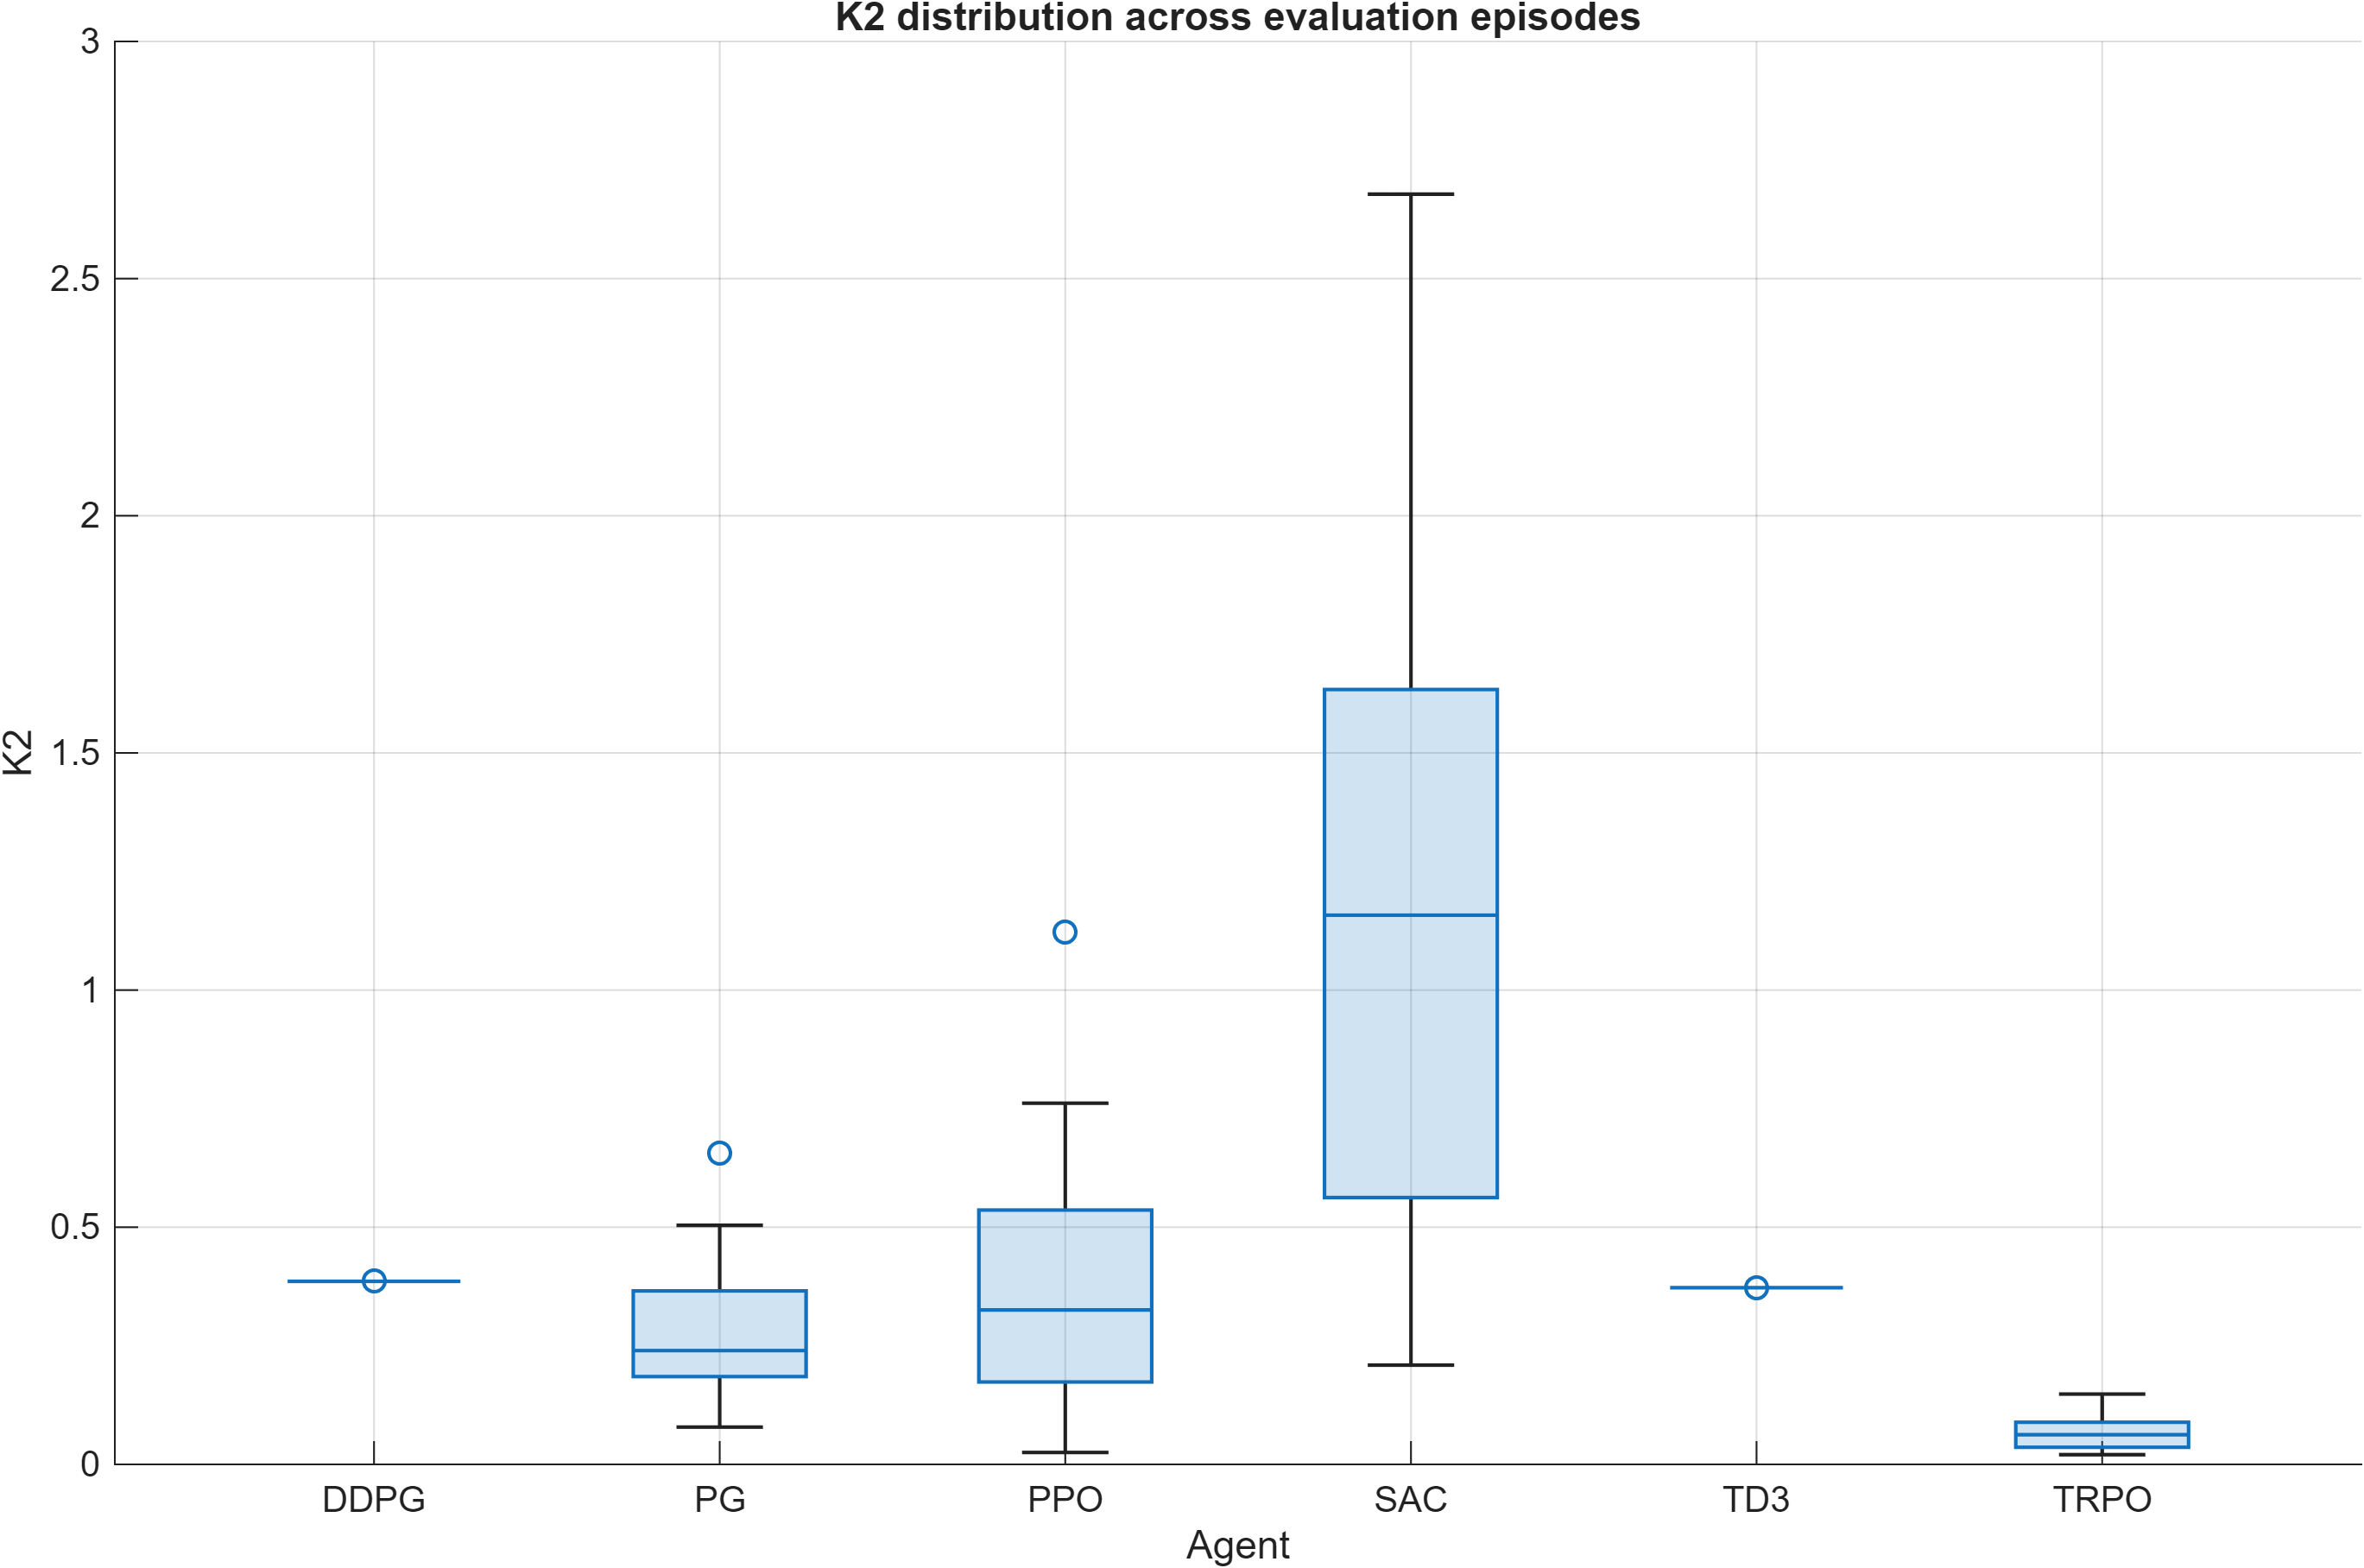
\includegraphics[width=\linewidth]{Figures/boxplot_K2.png}
    \caption{K2: Mean Squared EE Position Error}
    \label{fig:boxplot_k2}
  \end{subfigure}
  \hfill
  \begin{subfigure}{0.48\textwidth}
    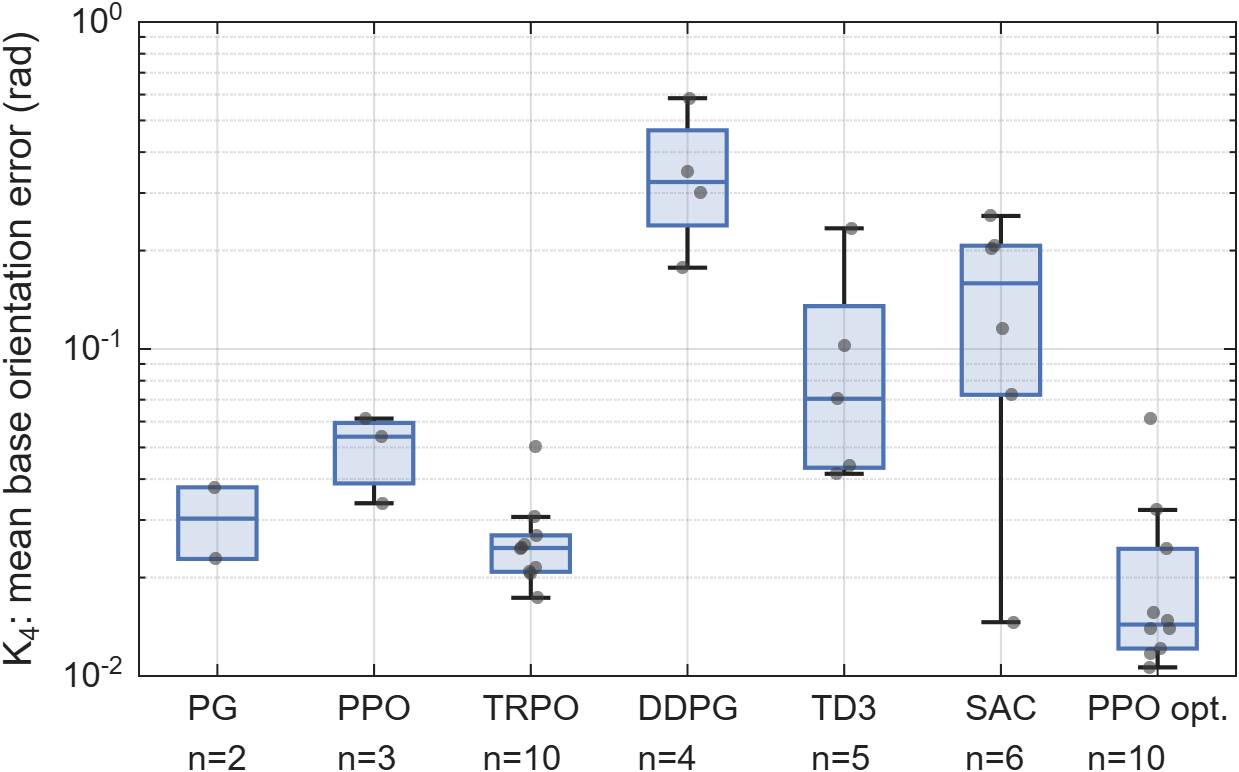
\includegraphics[width=\linewidth]{Figures/boxplot_K4.png}
    \caption{K4: Mean Base Orientation Error}
    \label{fig:boxplot_k4}
  \end{subfigure}
  \\[6pt]
  \begin{subfigure}{0.48\textwidth}
    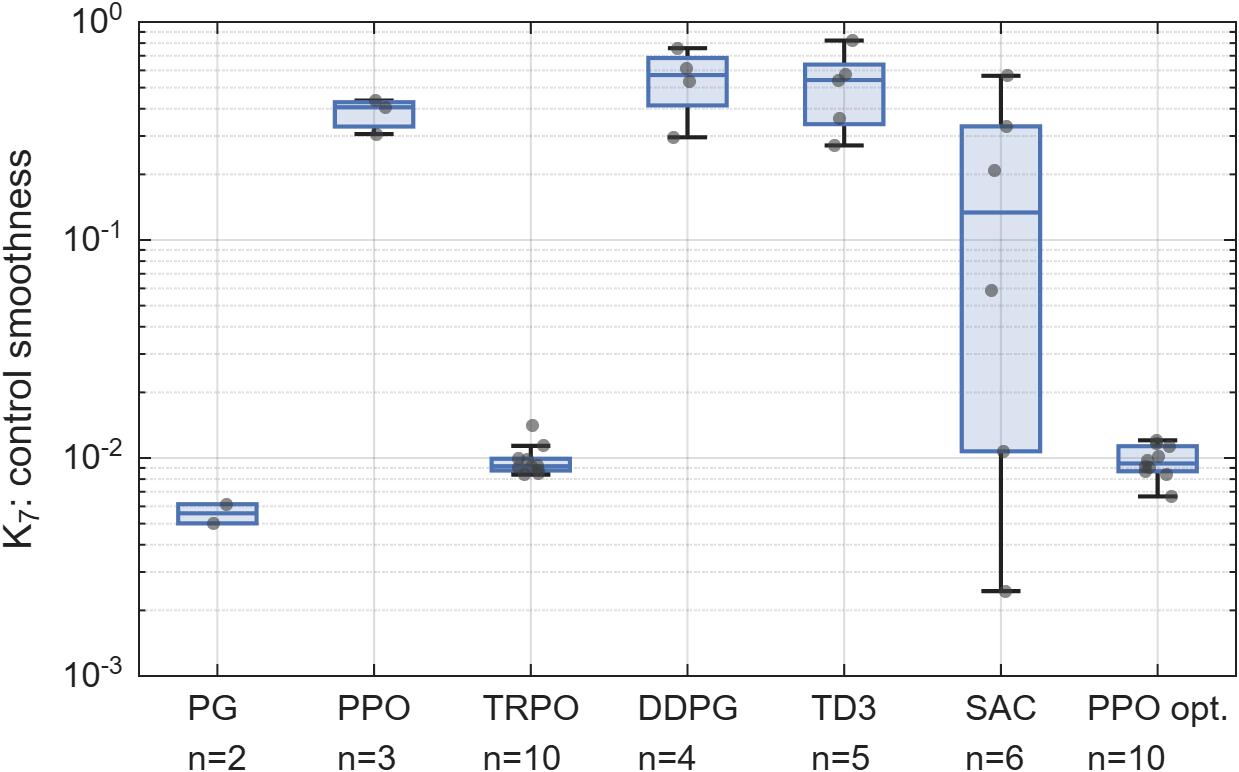
\includegraphics[width=\linewidth]{Figures/boxplot_K7.png}
    \caption{K7: Control Smoothness (Norm.\ Jerk)}
    \label{fig:boxplot_k7}
  \end{subfigure}
  \hfill
  \begin{subfigure}{0.48\textwidth}
    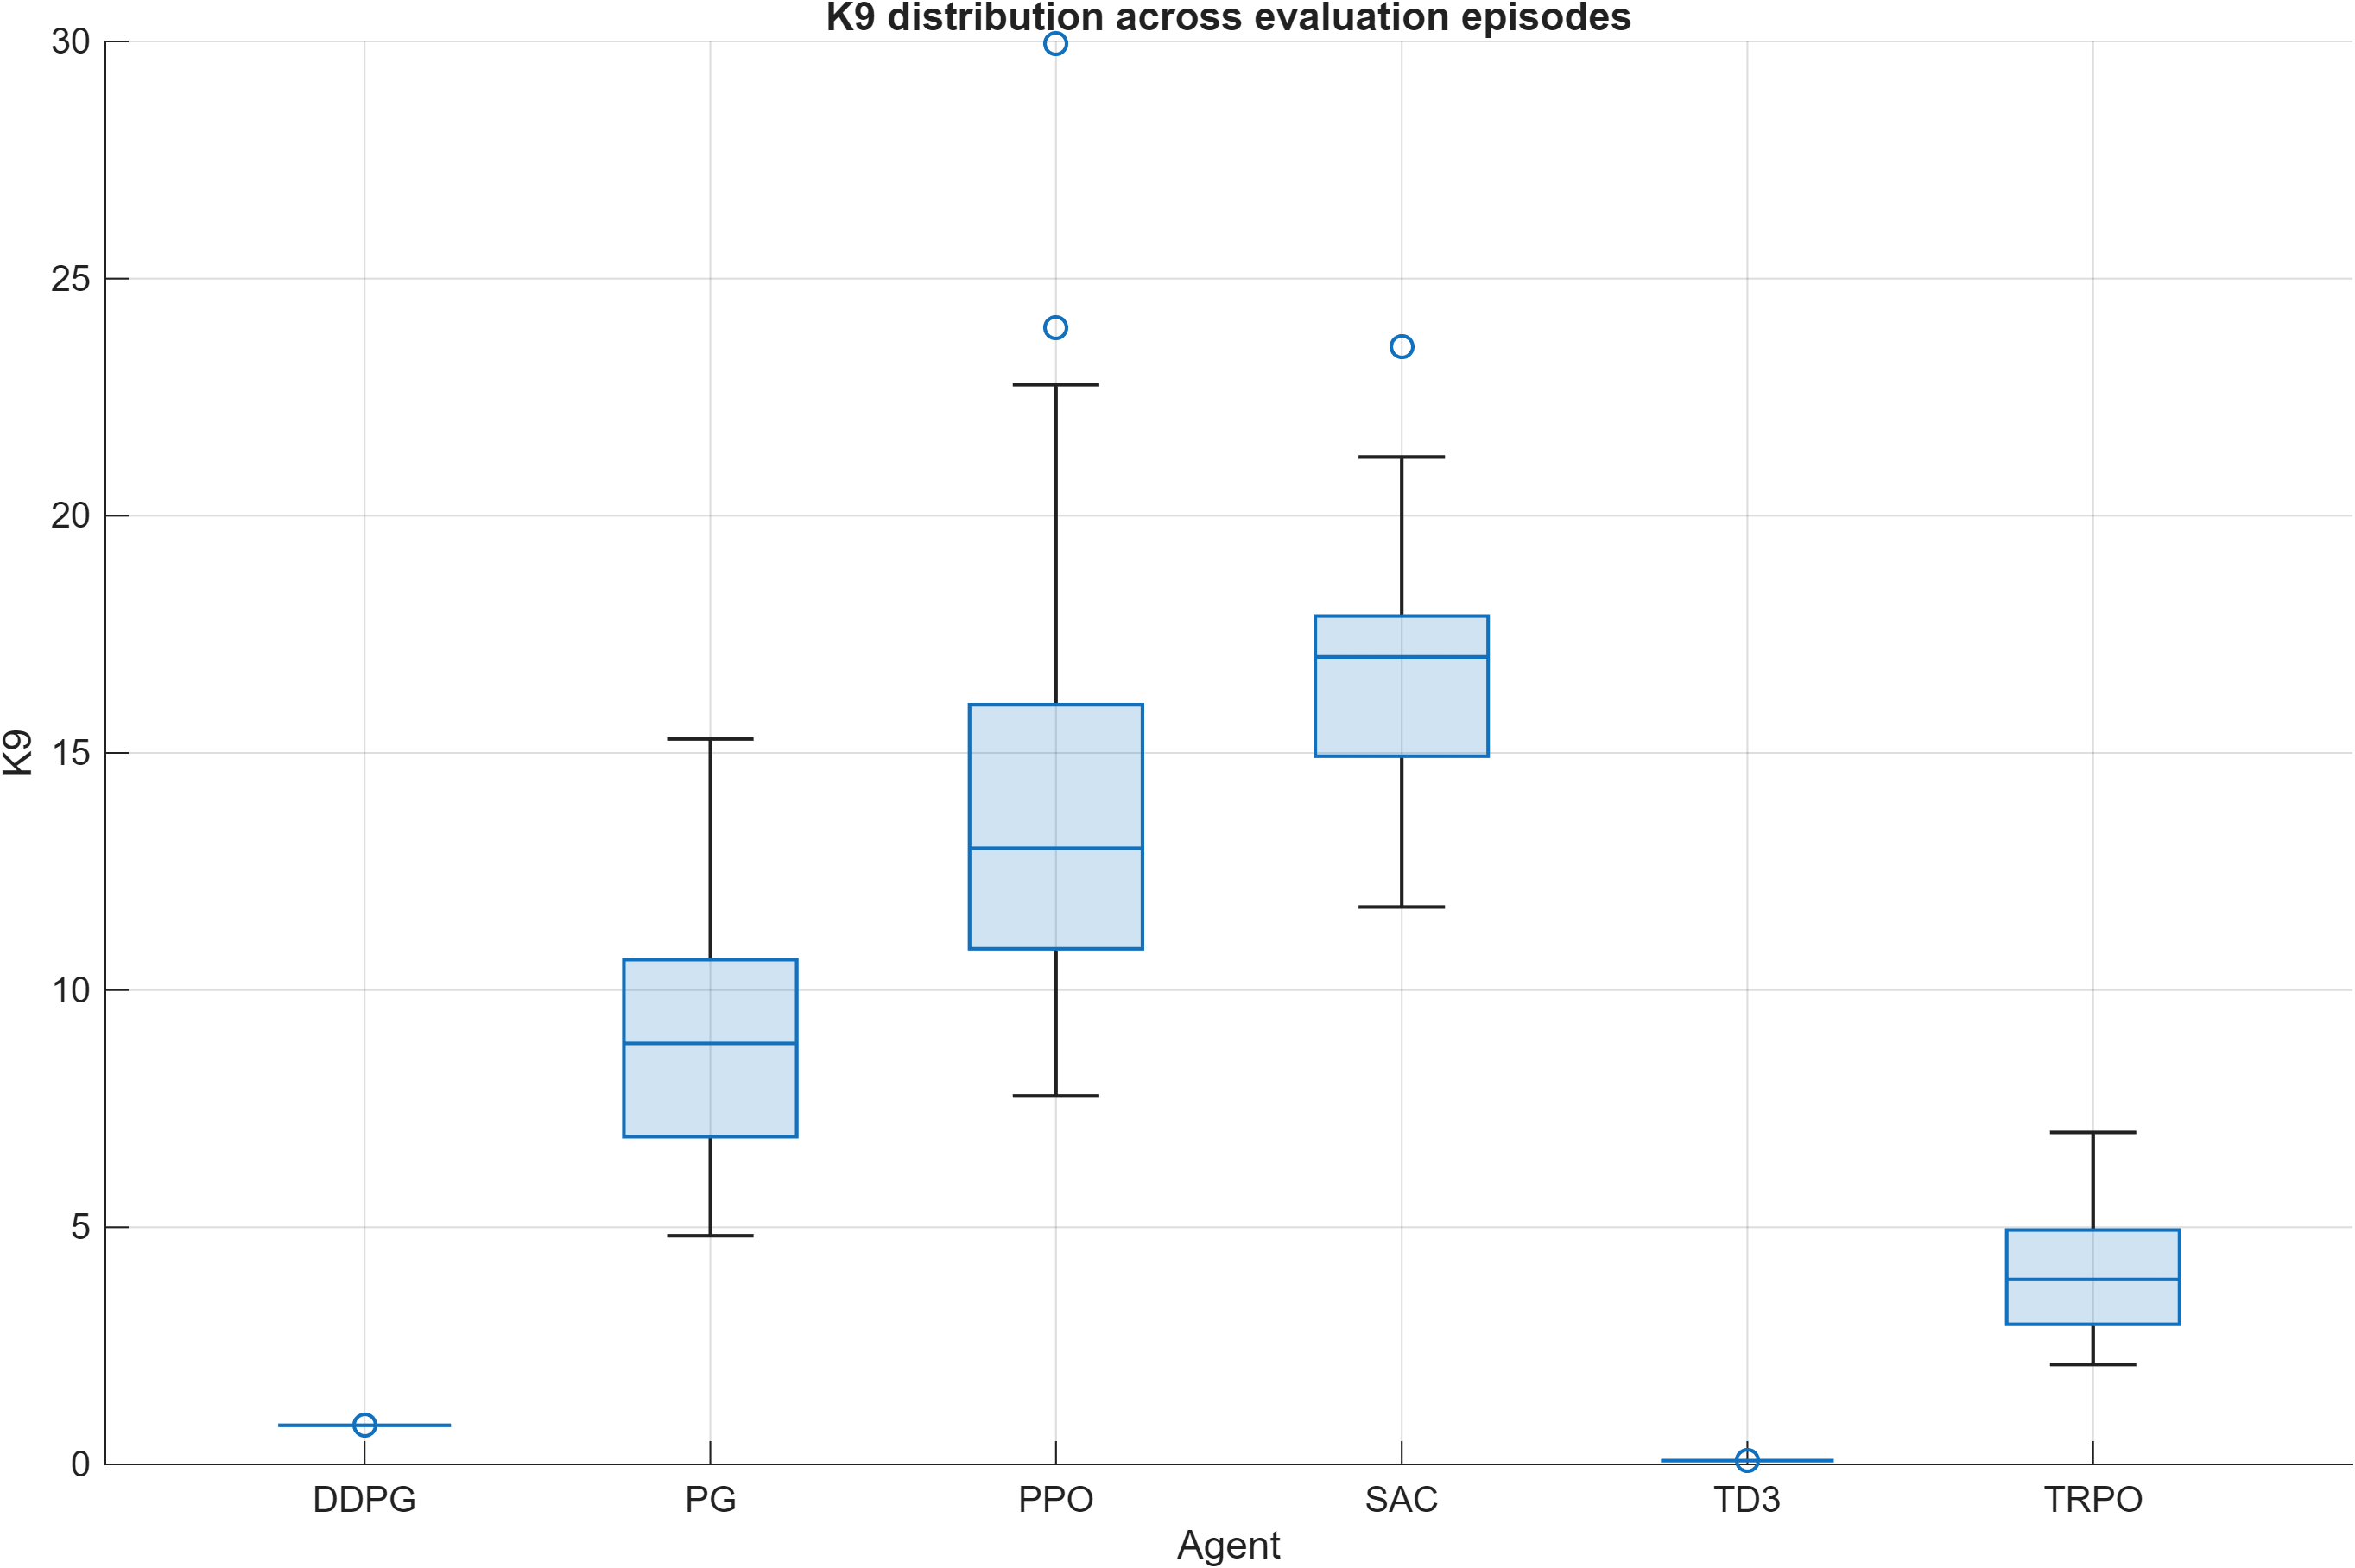
\includegraphics[width=\linewidth]{Figures/boxplot_K9.png}
    \caption{K9: Energy Consumption}
    \label{fig:boxplot_k9}
  \end{subfigure}
  \caption{\hltwo{[R2.13]} Boxplots of selected KPI distributions over 30 evaluation episodes per agent.
    Each box spans the interquartile range (IQR); the centre line marks the median;
    whiskers extend to 1.5\,$\times$\,IQR; circles denote outliers.
    PPO consistently achieves low tracking error (K2) and smooth control (K7) with small spread,
    while PG and SAC show high variability. The low K9 values for TD3 and DDPG reflect
    insufficient actuation rather than energy efficiency.}
  \label{fig:boxplots}
\end{figure*}

\begin{figure*}[!t]
  \centering
  \begin{subfigure}{0.48\textwidth}
    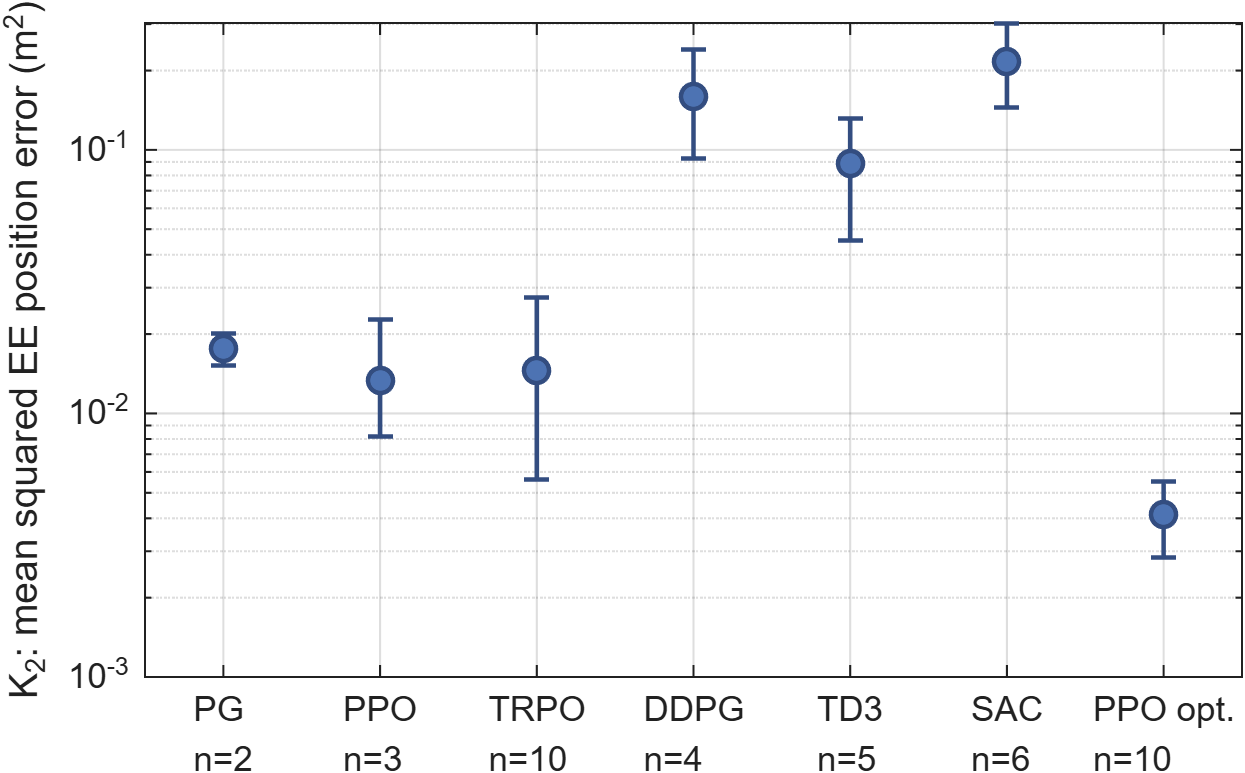
\includegraphics[width=\linewidth]{Figures/ci_K2.png}
    \caption{K2: Mean Squared EE Position Error}
    \label{fig:ci_k2}
  \end{subfigure}
  \hfill
  \begin{subfigure}{0.48\textwidth}
    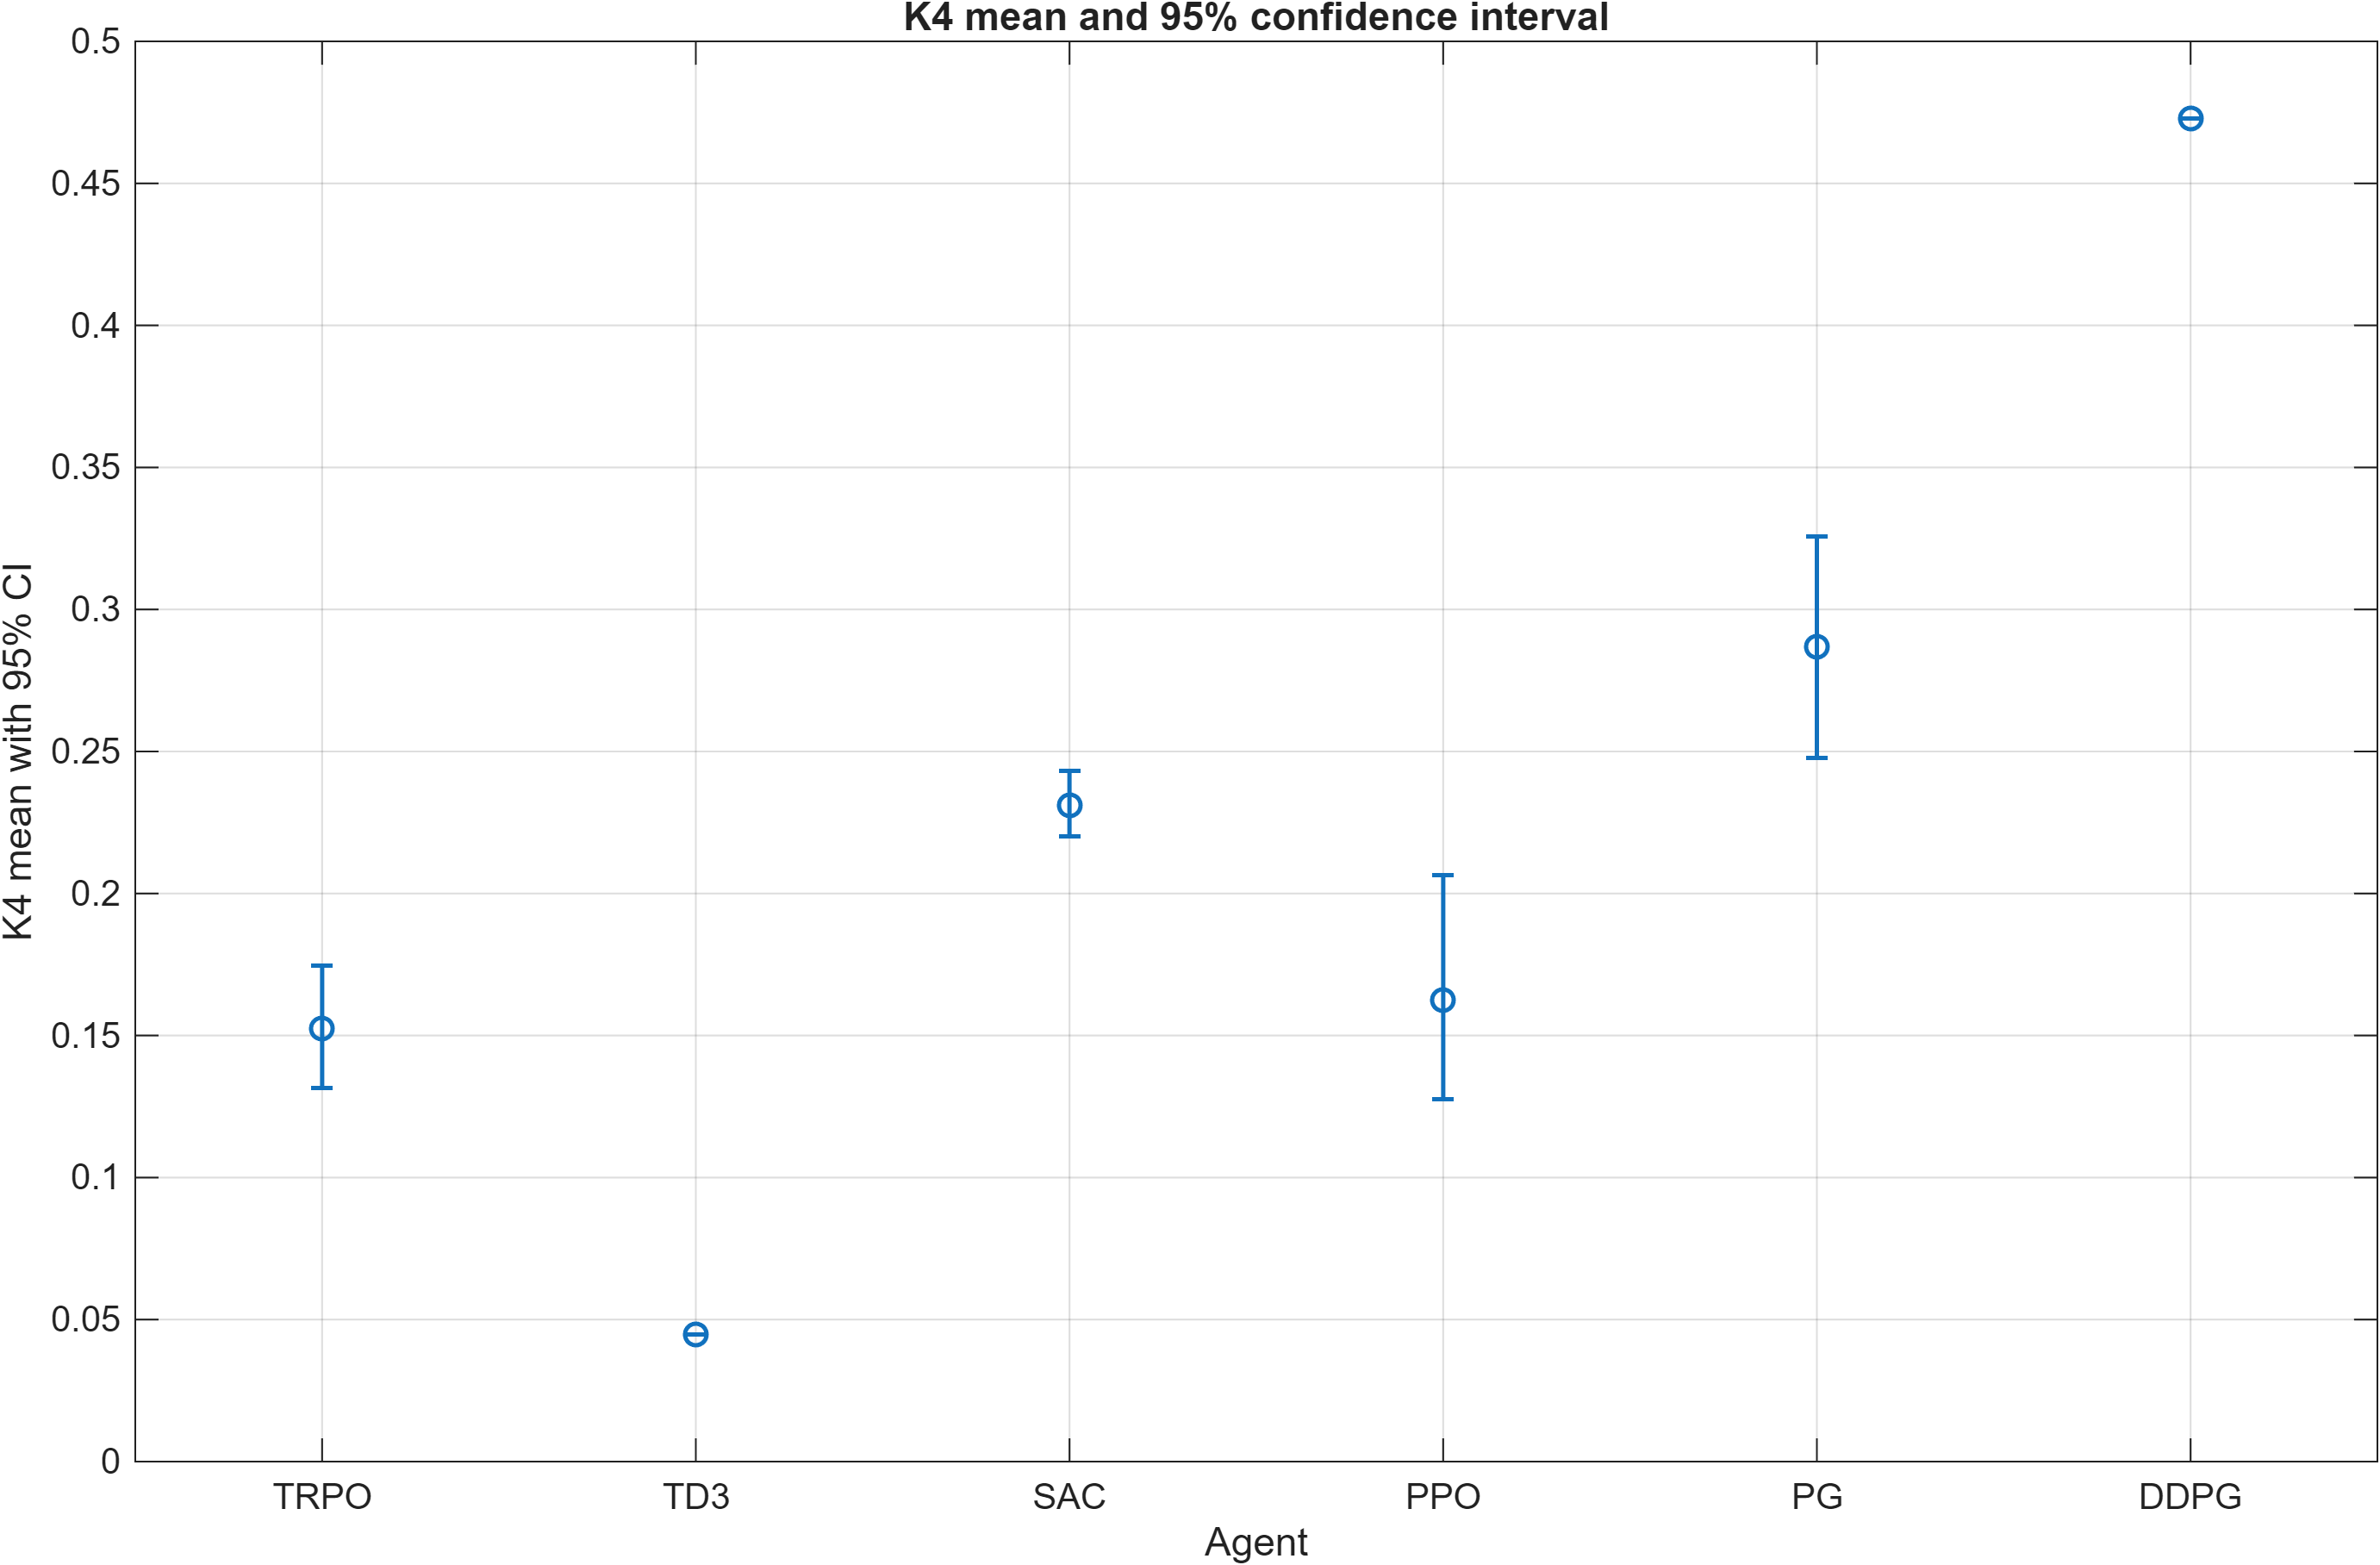
\includegraphics[width=\linewidth]{Figures/ci_K4.png}
    \caption{K4: Mean Base Orientation Error}
    \label{fig:ci_k4}
  \end{subfigure}
  \\[6pt]
  \begin{subfigure}{0.48\textwidth}
    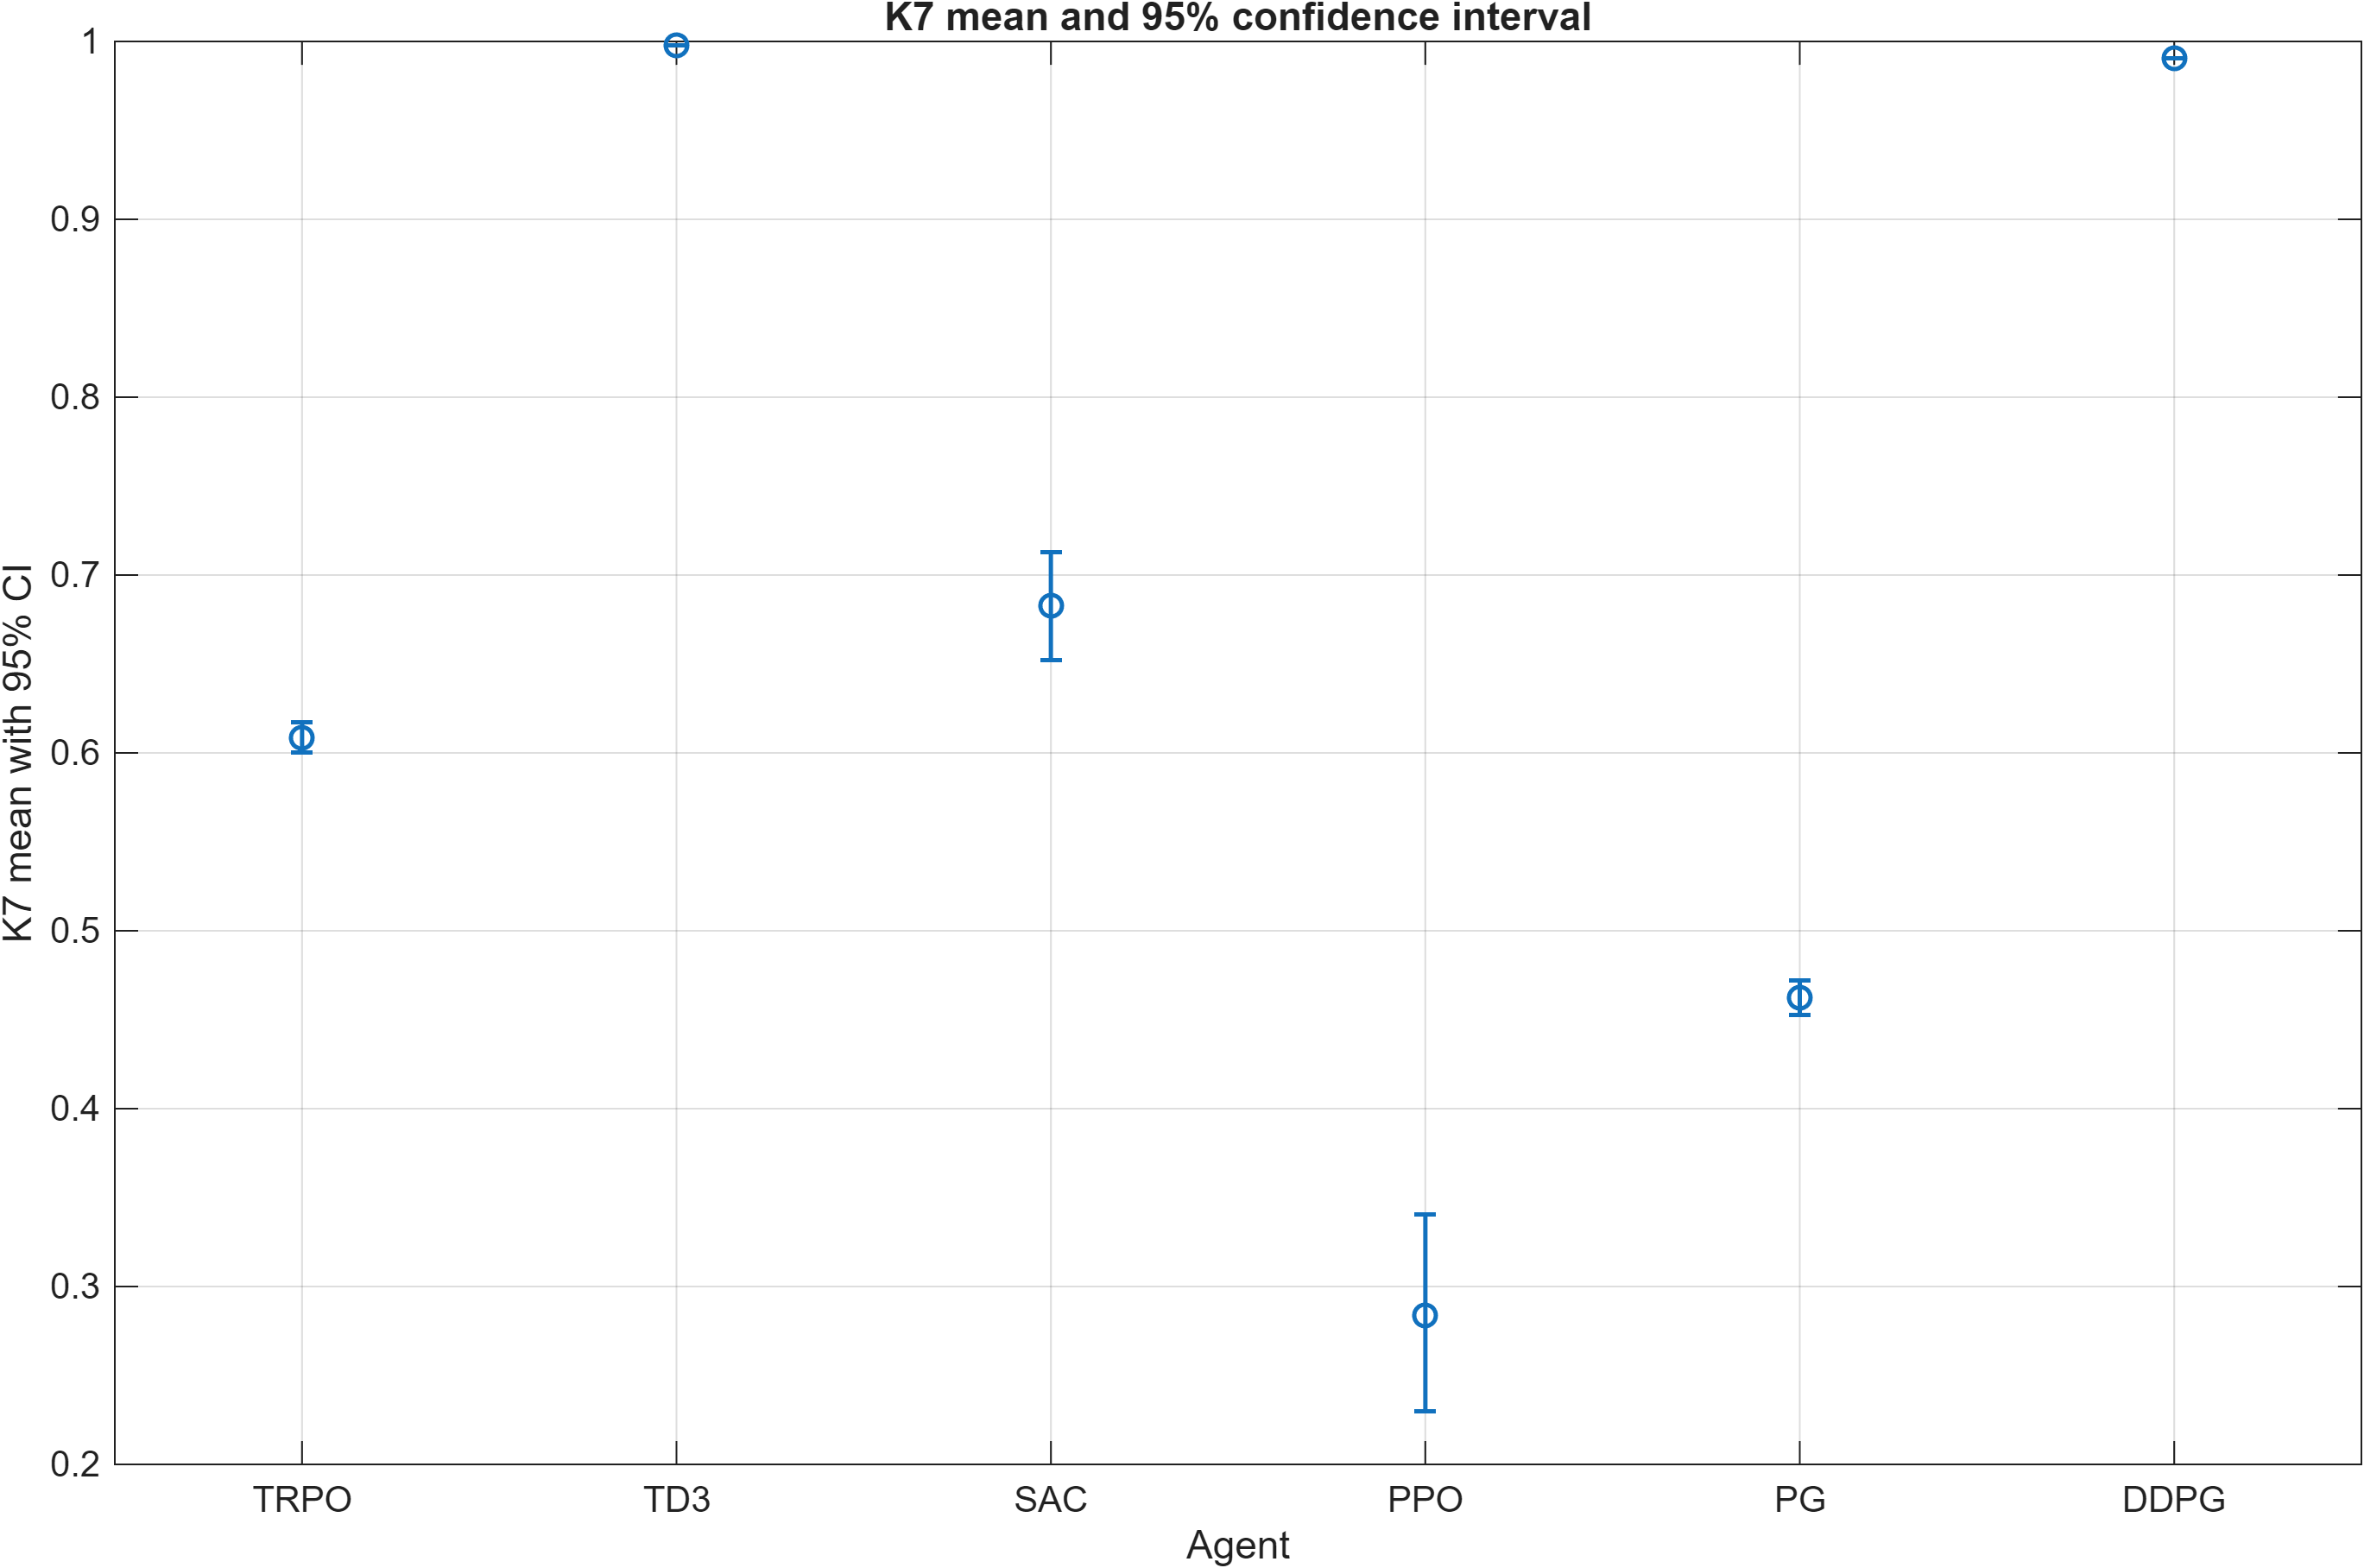
\includegraphics[width=\linewidth]{Figures/ci_K7.png}
    \caption{K7: Control Smoothness (Norm.\ Jerk)}
    \label{fig:ci_k7}
  \end{subfigure}
  \hfill
  \begin{subfigure}{0.48\textwidth}
    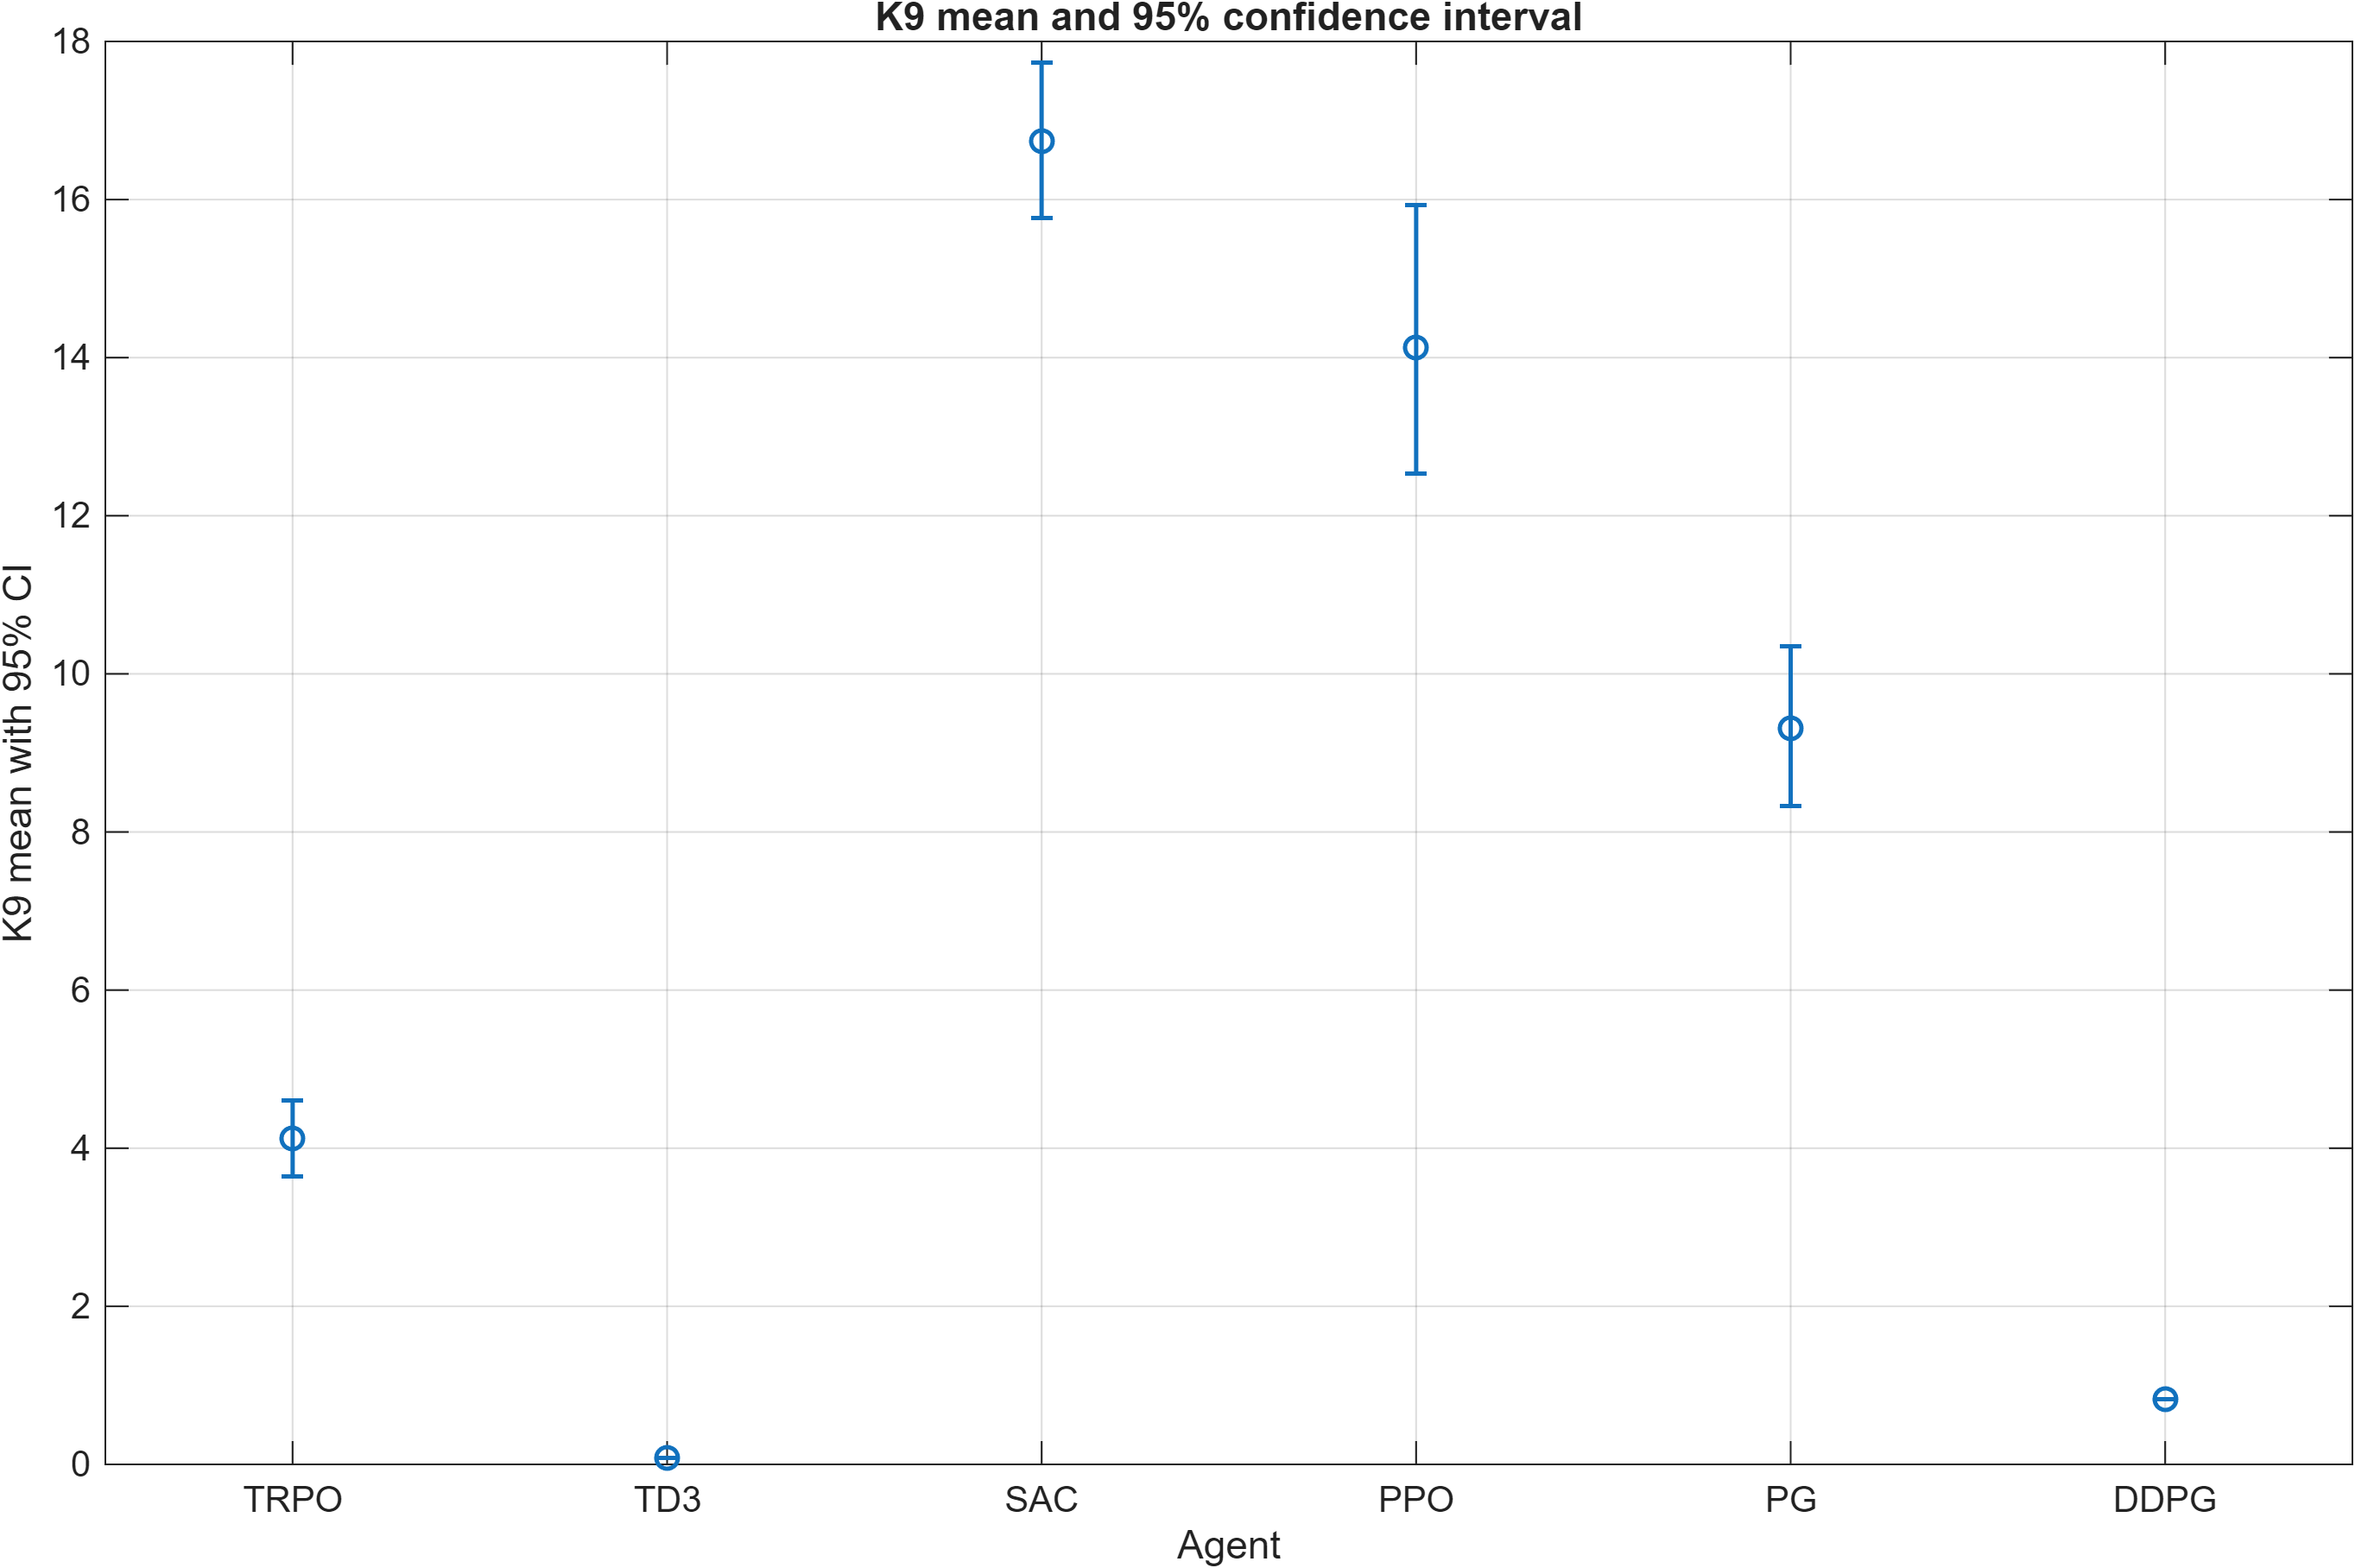
\includegraphics[width=\linewidth]{Figures/ci_K9.png}
    \caption{K9: Energy Consumption}
    \label{fig:ci_k9}
  \end{subfigure}
  \caption{\hltwo{[R2.12]} 95\% bootstrap confidence intervals for selected KPIs across all agents
    (30 evaluation episodes per agent).
    Narrow intervals for TD3 and DDPG reflect near-constant behaviour (policy collapse),
    whereas PPO's intervals are tight despite exploring the full workspace.
    TRPO and PPO show overlapping intervals for K4 (base orientation), consistent with
    the non-significant Wilcoxon result ($p=0.926$).}
  \label{fig:ci_plots}
\end{figure*}

\section{Optimization of the PPO Agent}
Based on the comparison in Section~\ref{comparison}, PPO is selected for further tuning. The PPO agent used so far corresponds to the default configuration provided by MATLAB's Reinforcement Learning Toolbox example \cite{b4}, with minimal manual adjustment. The following modifications target three objectives: faster convergence, lower tracking and base-orientation errors, and avoidance of the remaining joint-limit violations. The tuning involves both network architecture and hyperparameters.



\begin{figure*}[!t]
	\centering
	\begin{subfigure}{0.48\textwidth}
		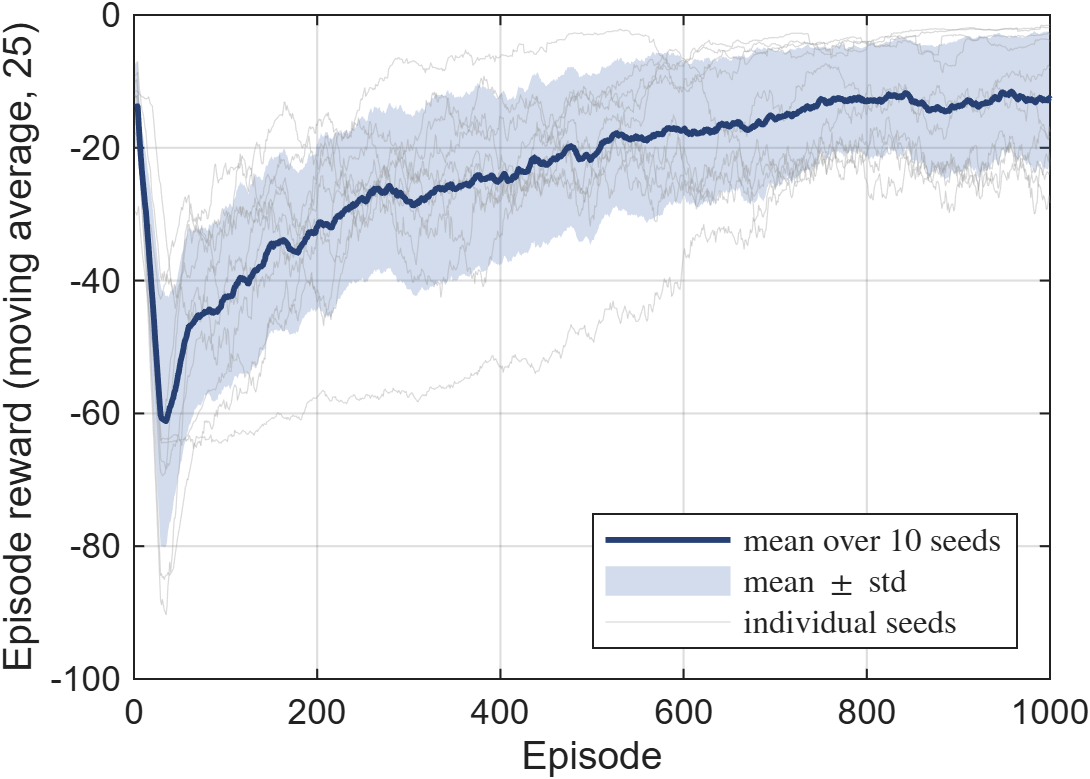
\includegraphics[width=\linewidth,height=0.25\textheight]{Figures/trainingsverlauf_ppo_default.png}
		\caption{PPO (Default)}
		\label{fig:training_ppo_default}
	\end{subfigure}
	\hfill
	\begin{subfigure}{0.48\textwidth}
		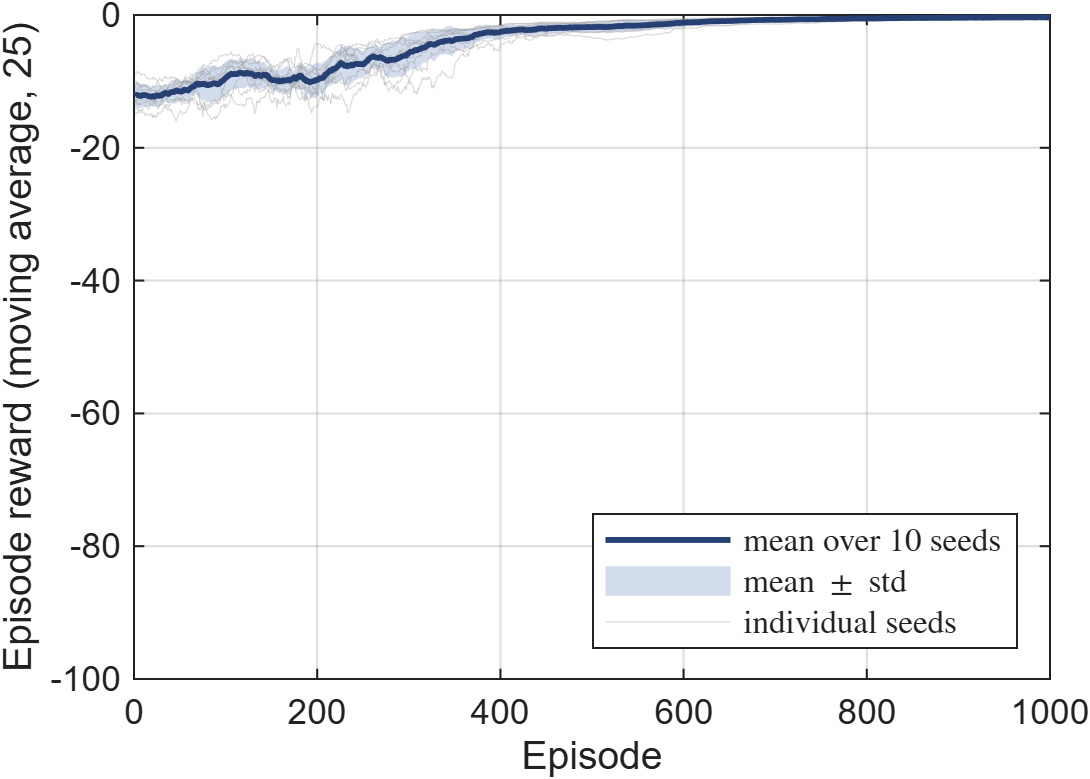
\includegraphics[width=\linewidth, height=0.25\textheight]{Figures/trainingsverlauf_ppo_optimized.png}
		\caption{PPO (Optimized)}
		\label{fig:training_ppo_opt}
	\end{subfigure}
	\caption{Comparison of episodic rewards for default and optimized PPO agents.
  (a) Episode reward evolution during training using the default PPO hyperparameters. 
  (b) Episode reward evolution using the optimized PPO configuration.
 The optimized configuration shows faster convergence and a higher average episodic return than the
 default configuration.}
	\label{fig:training_ppo_compare}
\end{figure*}
\noindent

\begin{roverlaphl}
\hloverlap{[R2.10/R3.8]} \textbf{Network architecture.} The default PPO agent uses two hidden layers of 128
units each with ReLU activations for both the policy and the value network. Variants with deeper and wider networks and with alternative activation functions were evaluated. The selected architecture uses three hidden layers of sizes $[256, 256, 128]$ for the policy network and two hidden layers of sizes $[256, 128]$ for the value network. The additional depth and capacity of the policy network reduce the tracking error and the base-orientation error (cf.\ \autoref{tab:ppo_optimization_kpi}) for the 23-dimensional state input \cite{b4}. Layer normalization is applied to the first layer to compensate for the different scales of the input features (e.g., joint angles versus orientation quaternions). The activation function is kept as ReLU. The networks are defined explicitly rather than through the toolbox default constructor.

\textbf{Hyperparameter Tuning:} The optimization followed a coordinate-wise grid search: each hyperparameter was swept across a discrete set of candidate values while all others were held at their current best, and the configuration yielding the highest mean episodic reward over the final 50 training episodes (out of $N_{\text{train}}=1000$) was selected. In total, 16 training runs of 1000 episodes each were conducted during this tuning phase. The swept parameters, their candidate values, and the selected values are as follows:
\begin{itemize}
  \item \textbf{Actor learning rate} — candidates: $\{1\!\times\!10^{-3},\;5\!\times\!10^{-4}\}$; selected: $5\!\times\!10^{-4}$. The lower rate reduced overshooting in policy gradient updates, improving convergence stability.
  \item \textbf{Critic learning rate} — candidates: $\{1\!\times\!10^{-3},\;5\!\times\!10^{-4}\}$; selected: $1\!\times\!10^{-3}$. A higher critic learning rate allowed the value function to track the evolving policy more closely, providing more accurate advantage estimates.
  \item \textbf{Entropy loss weight} — candidates: $\{1\!\times\!10^{-2},\;1\!\times\!10^{-3}\}$; selected: $1\!\times\!10^{-3}$. A small entropy bonus discouraged premature convergence to a suboptimal deterministic policy and encouraged the agent to discover strategies such as coordinated joint motions that cancel base momentum, without causing aimless exploration.
  \item \textbf{Experience horizon} — candidates: $\{512,\;1024,\;2048\}$; selected: $1024$. A moderate rollout horizon provided sufficient trajectory information per update while keeping memory requirements and update latency manageable.
  \item \textbf{Mini-batch size} — candidates: $\{128,\;256\}$; selected: $256$. Larger batches provided more stable gradient estimates per update, reducing training variance.
\end{itemize}

This process yielded a configuration that provided a more stable and higher-performing PPO agent. Notably, the asymmetric learning rates --- a slower actor ($5\!\times\!10^{-4}$) paired with a faster critic ($1\!\times\!10^{-3}$) --- reflect the different roles of the two networks: the value function must adapt quickly to policy changes, while conservative actor updates prevent destabilizing the learned control strategy.
\end{roverlaphl}

\subsection{Circular Trajectory}

\textbf{Training outcome.} The effect of the modifications can be seen in the training curves (see~\autoref{fig:training_ppo_compare}). The default PPO agent's episodic return increases initially and then plateaus around $-2$ per episode with high variance over the remaining training, indicating convergence to a suboptimal policy. In contrast, the optimized PPO agent's return continues to increase and converges to a higher value (closer to zero) with reduced variance. Table~\ref{tab:ppo_optimization_kpi} reports the KPI averages over $N_{\mathrm{eval}} = 30$ evaluation episodes for PPO with the default and the optimized configurations. The mean episodic return $K_1$ increases from $-2.23$ for the default PPO to $-0.43$ for the optimized PPO, an increase by a factor of approximately five. The reduced variance indicates that the improvement is consistent across episodes rather than driven by a few outliers.

\begin{figure*}[!t]
    \centering
    \begin{subfigure}{0.48\textwidth}
        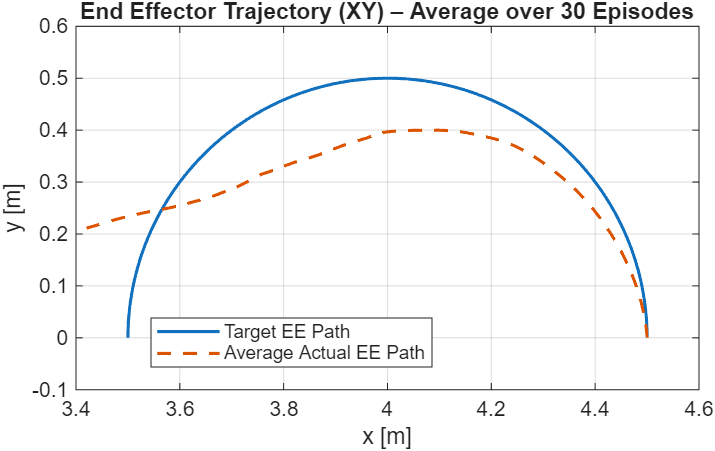
\includegraphics[width=\linewidth]{Figures/soll_vs_ist_kreisbahn.png}
        \caption{PPO (Default)}
        \label{fig:traj_default}
    \end{subfigure}
    \hfill
    \begin{subfigure}{0.48\textwidth}
        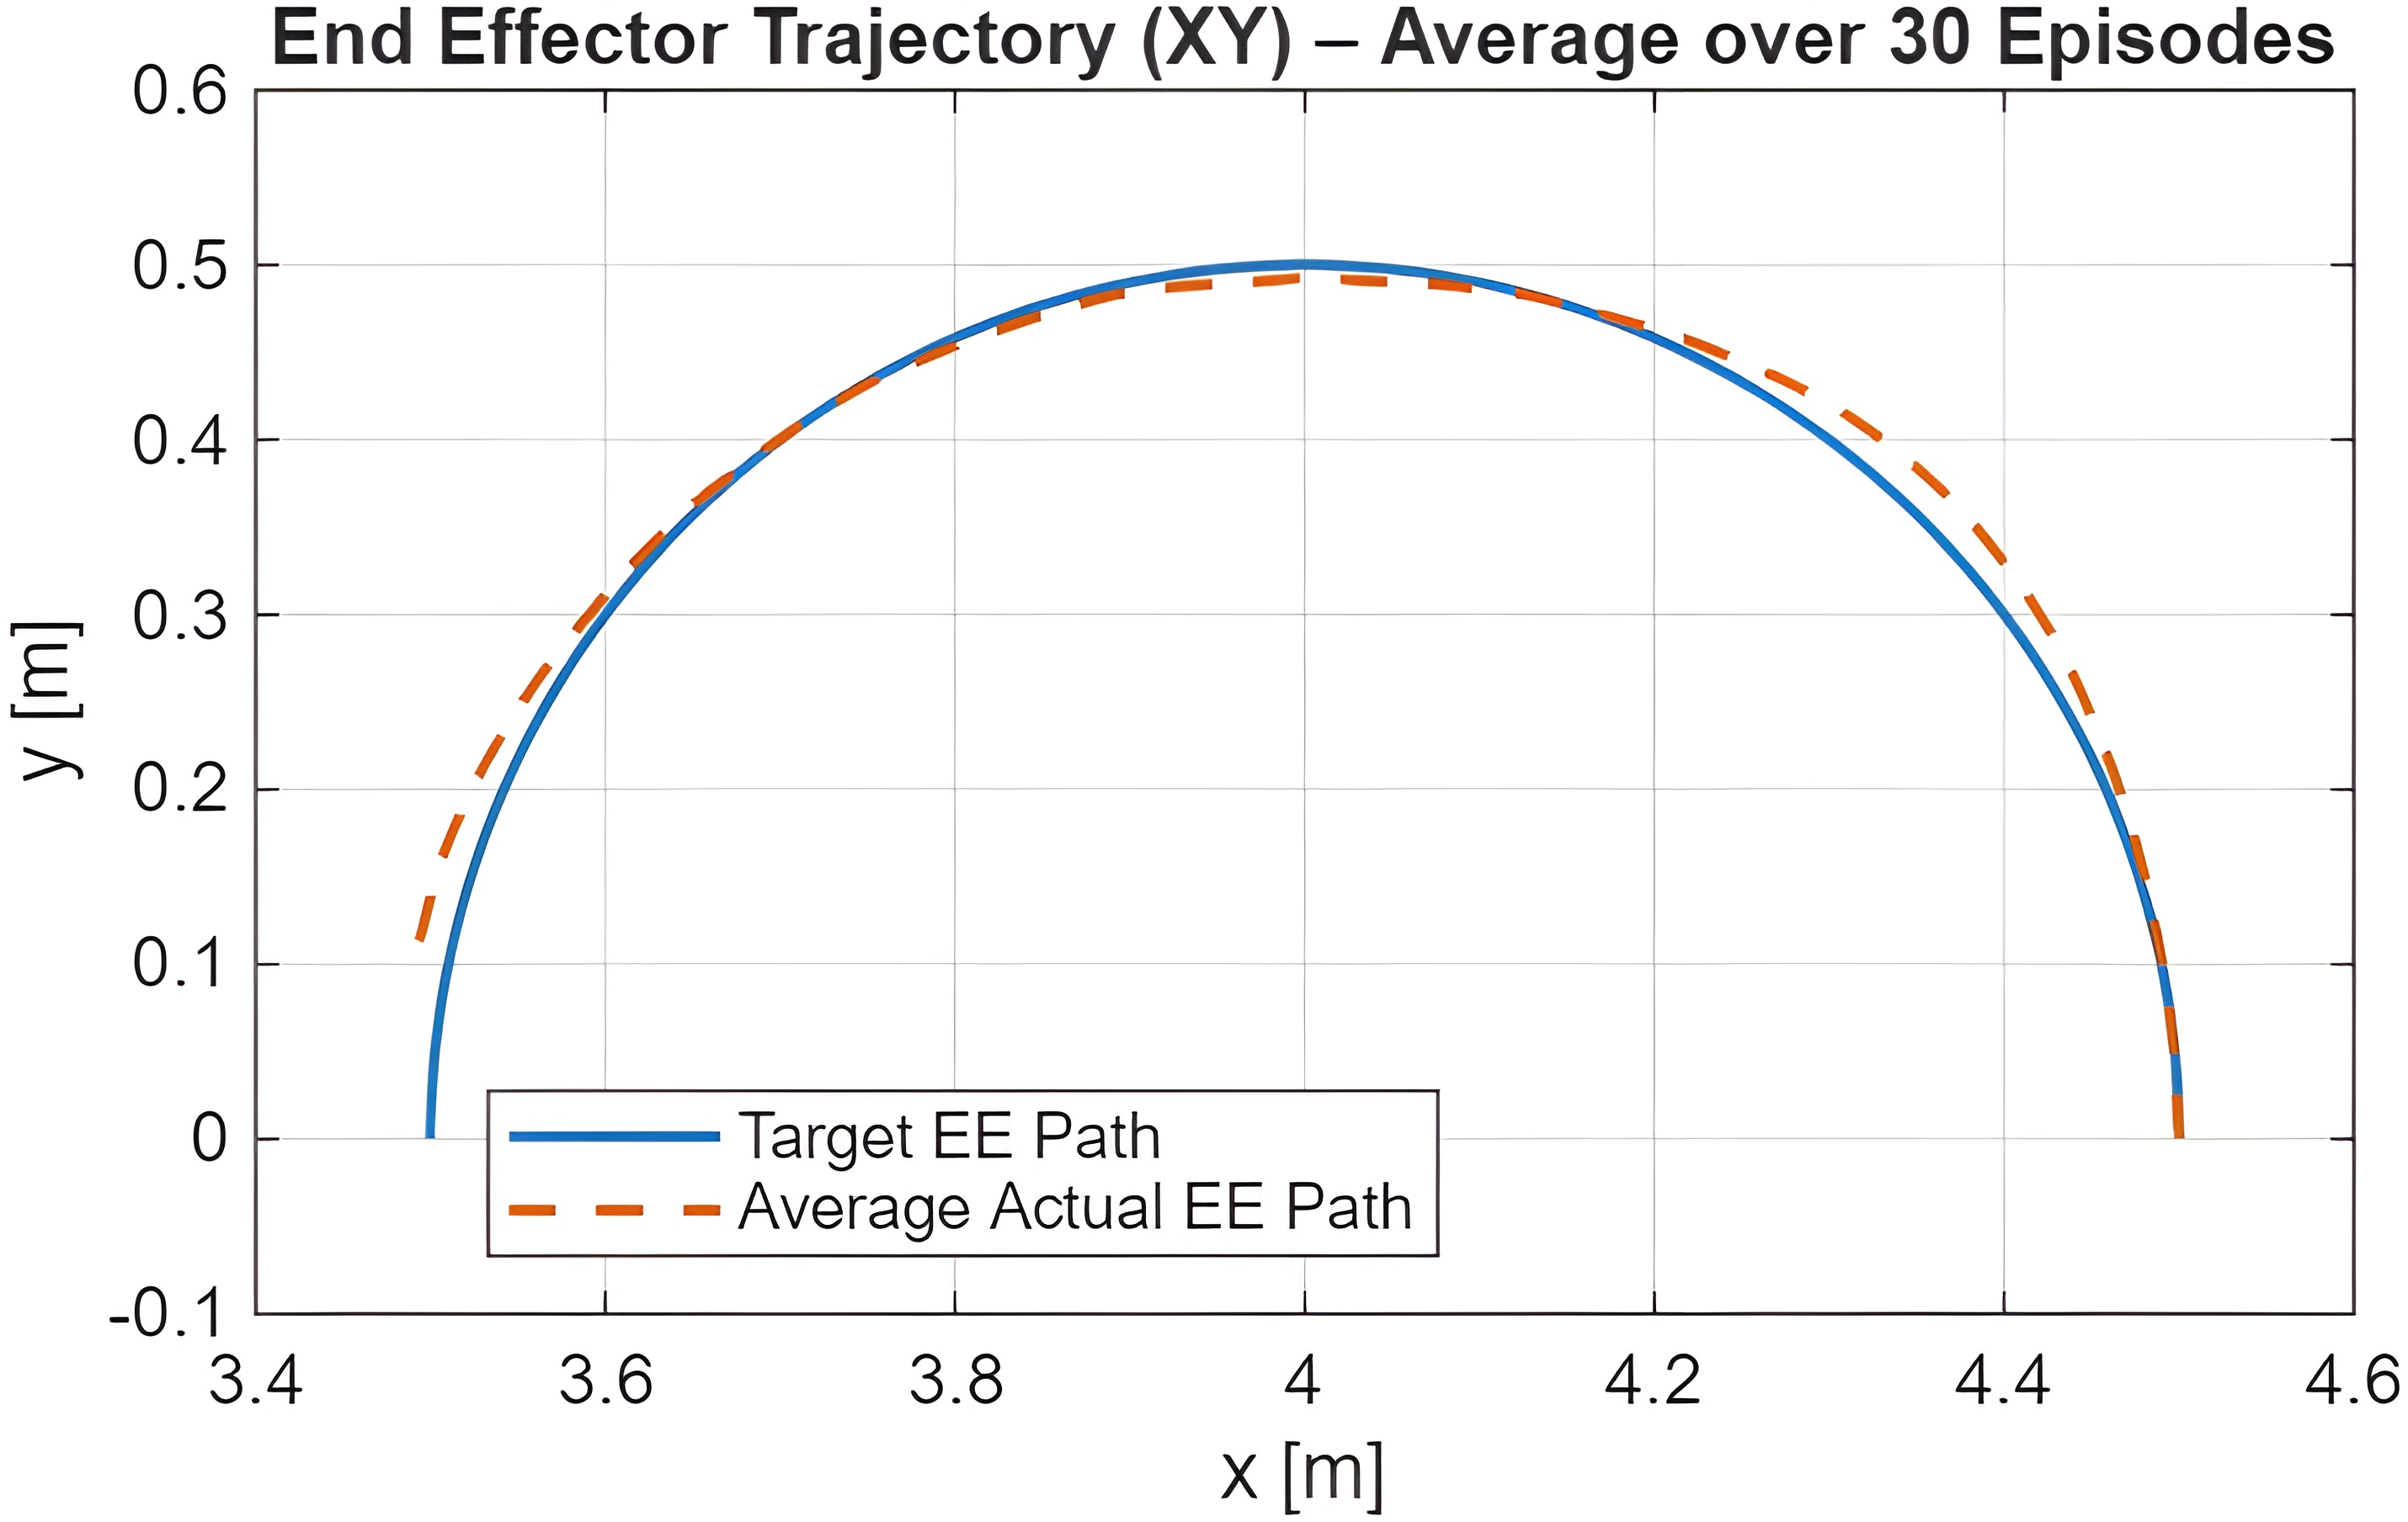
\includegraphics[width=\linewidth]{Figures/soll_vs_ist_kreisbahn_opt.png}
        \caption{PPO (Optimized)}
        \label{fig:traj_opt}
    \end{subfigure}
    \caption{Target/actual comparison of the end-effector trajectory in the XY plane.}
    \label{fig:trajektorie_xy_compare}
\end{figure*}

\begin{figure*}[!t]
    \centering
    \begin{subfigure}{0.48\textwidth}
        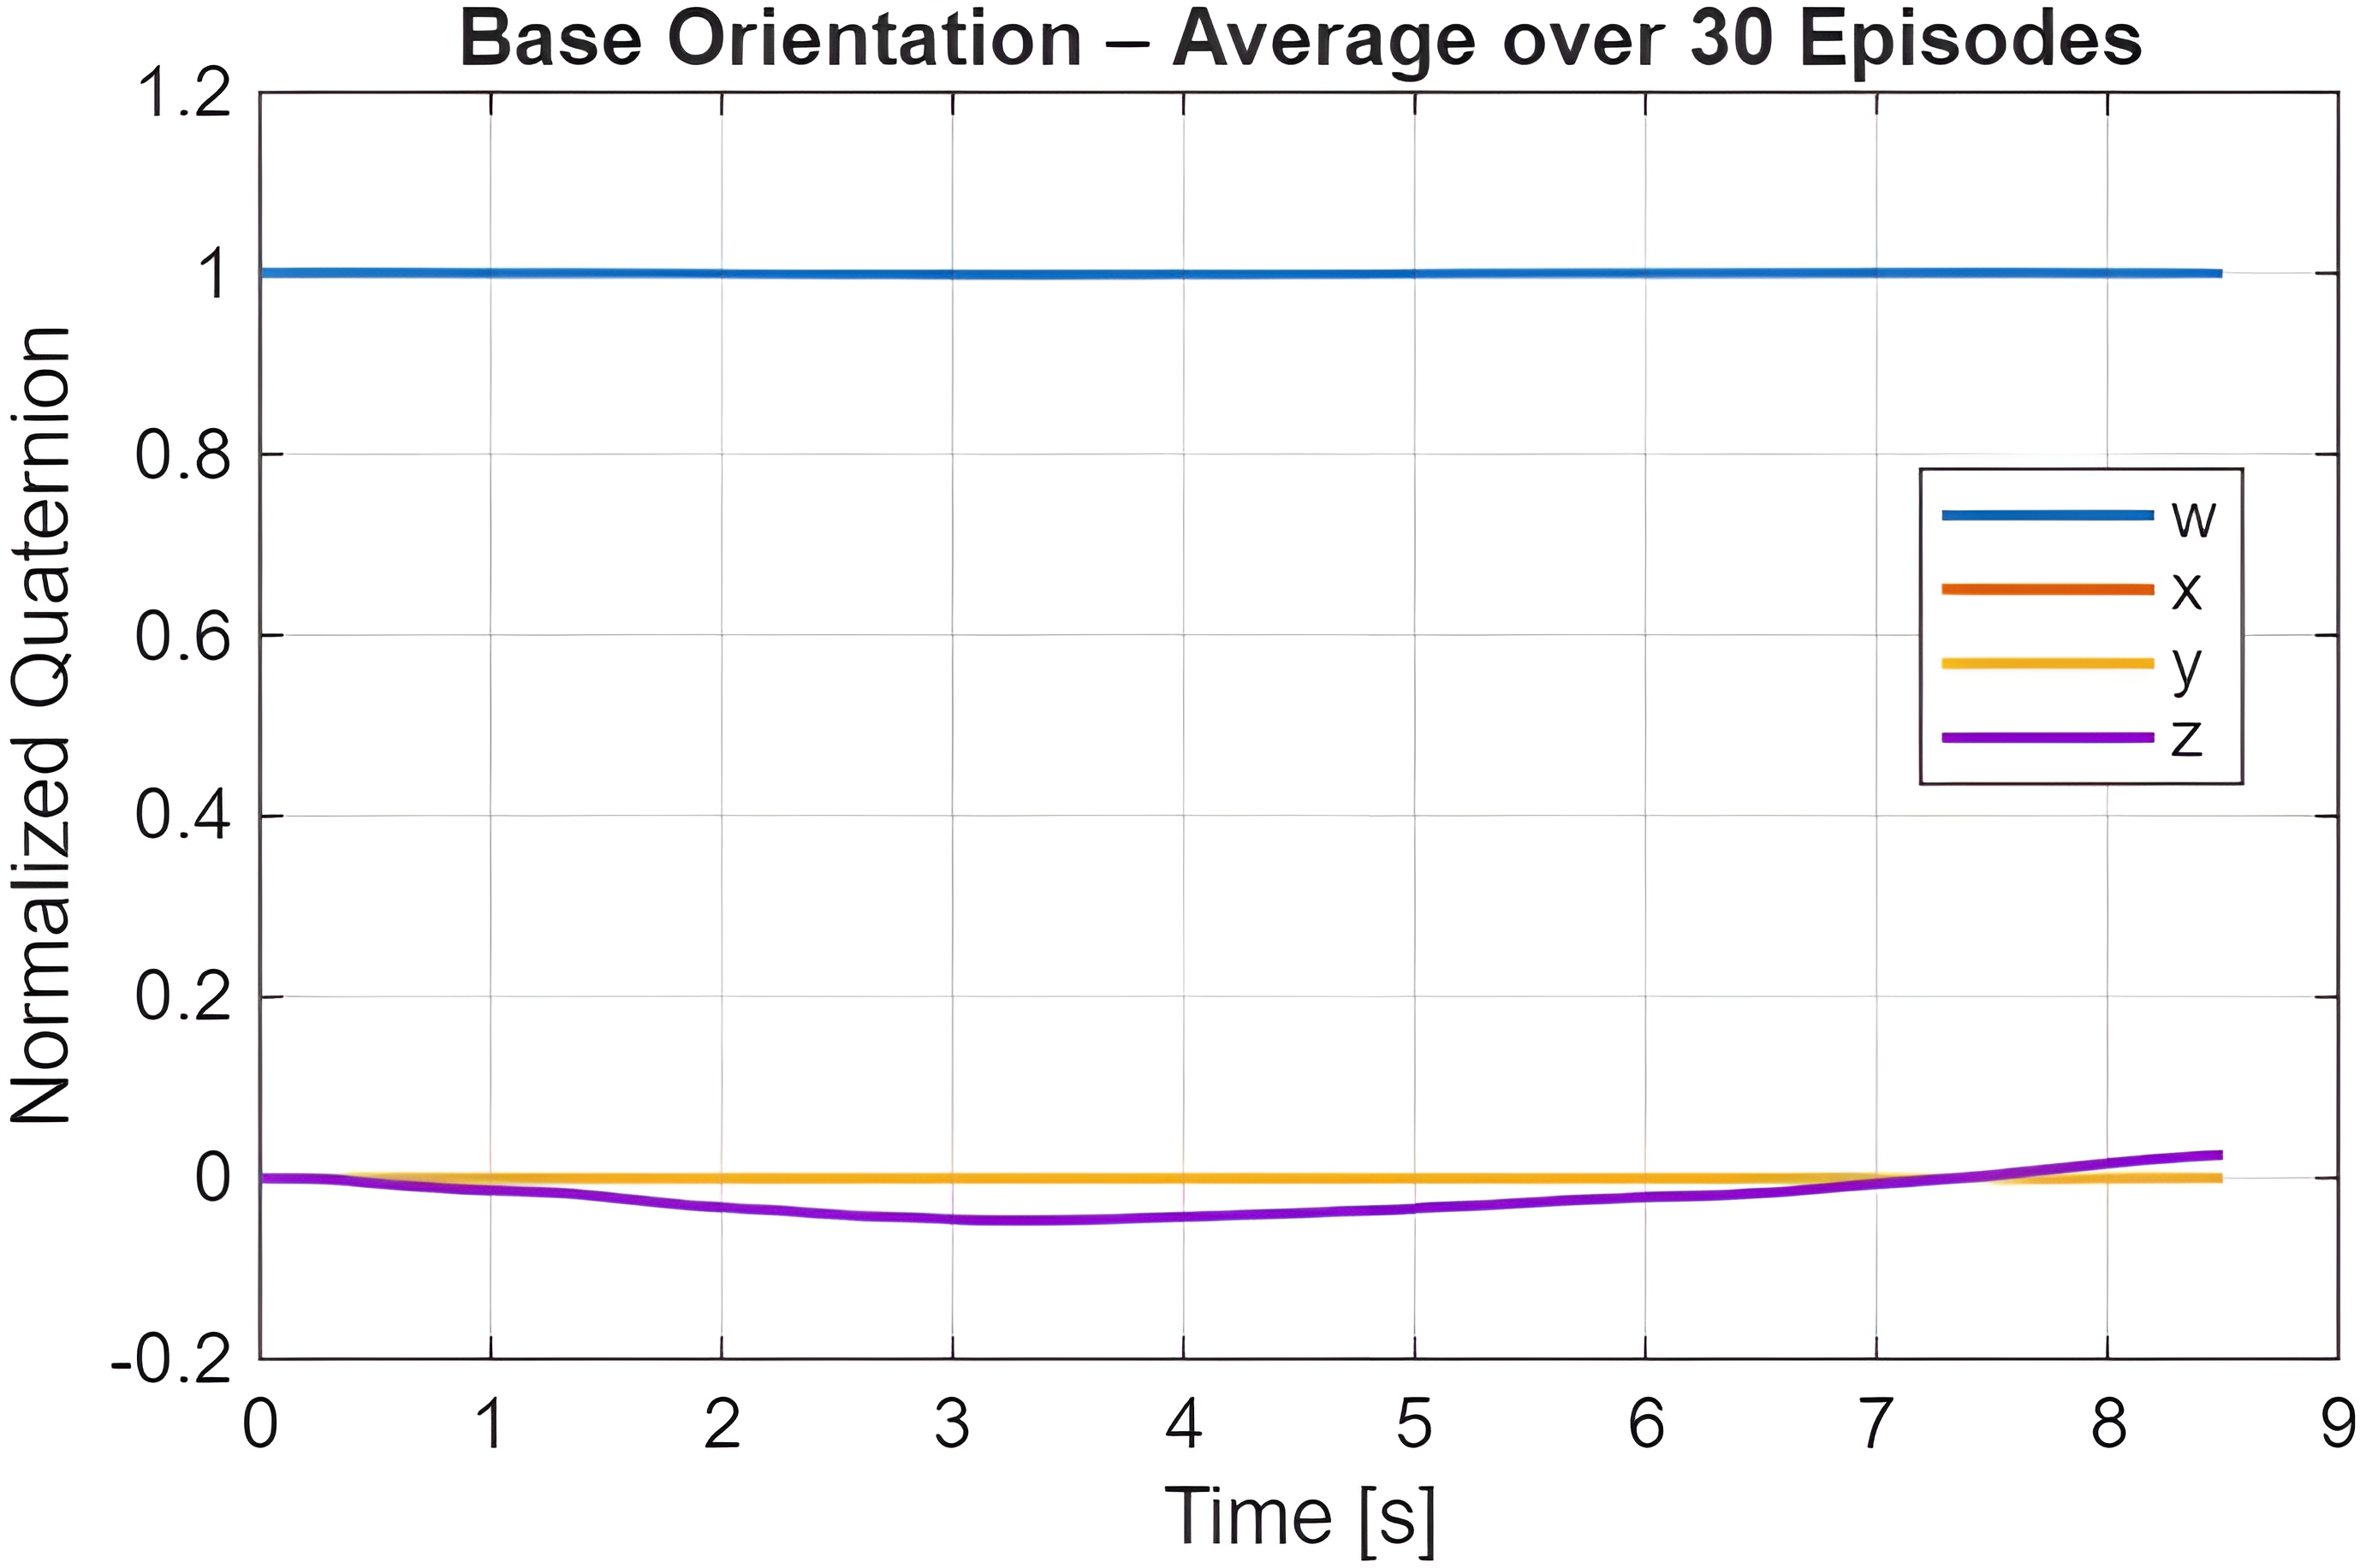
\includegraphics[width=\linewidth]{Figures/basis_orientaion_ppo.png}
        \caption{PPO (Default)}
        \label{fig:basis_default}
    \end{subfigure}
    \hfill
    \begin{subfigure}{0.48\textwidth}
        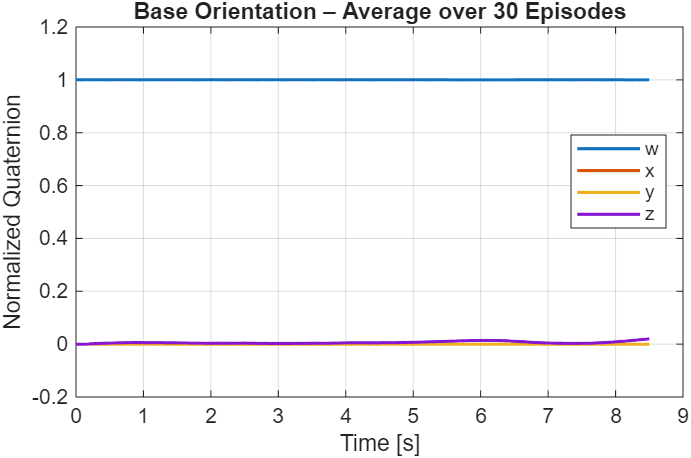
\includegraphics[width=\linewidth]{Figures/basis_orientation_ppo_optimized.png}
        \caption{PPO (Optimized)}
        \label{fig:basis_opt}
    \end{subfigure}
    \caption{Time evolution of the base orientation (quaternion components) during a test episode.}
    \label{fig:basis_orientation_compare}
\end{figure*}

\begin{table}[!b]
	\centering
	\caption{Performance of PPO agent before and after optimization. The optimized PPO improves most reported
		KPIs, with higher rewards, lower errors, no observed safety violations in the evaluation episodes, and smoother
		control.}
    \label{tab:ppo_optimization_kpi}
	\renewcommand{\arraystretch}{1.2}
	\setlength{\tabcolsep}{3pt}
	\begin{tabular}{lcc}
		\toprule
		\textbf{Metric (KPI)} & \textbf{PPO (Default)} & \textbf{PPO (Optimized)} \\
		\midrule
		Mean Episodic Reward (K1)        & $-2.23$  & $\mathbf{-0.43}$ \\
		Mean Squared EE Tracking Error (K2)      & 0.0257  & \textbf{0.0083} \\
		Max EE Tracking Error (K3)       & 0.4833   & \textbf{0.27} \\
		Mean Base Orientation Error (K4) & 0.0667  & \textbf{0.022} \\
		Collision Rate (K5)             & 0 & 0 \\
		Joint Limit Violation Rate (K6) & 0.0505 (5.1\%) & \textbf{0} \\
		Torque Smoothness (K7, jerk)     & 0.6812  & \textbf{0.351} \\
		Mean Base Angular Velocity (K8)  & 0.095  & \textbf{0.050} \\
		Energy Consumption (K9)          & 6.325  & \textbf{5.314} \\
		\bottomrule
	\end{tabular}
\end{table}

The reward improvement translates directly into task-level performance. \autoref{fig:trajektorie_xy_compare}
shows the end-effector path in the $XY$ plane: the default PPO deviates from the reference circle and exhibits oscillations, while the optimized PPO closely follows the reference. The mean squared tracking error $K_2$ decreases from $0.0257$ to $0.0083$ (a reduction of $67.7\%$), and the maximum error $K_3$ from $0.4833$ to $0.27$.

Base stabilization improves accordingly (\autoref{fig:basis_orientation_compare}): the mean orientation error $K_4$ decreases from $0.0667$ to $0.022$ (a factor of approximately three), and the mean angular velocity $K_8$ decreases from $0.095\,\mathrm{rad/s}$ to $0.050\,\mathrm{rad/s}$. The optimized agent uses arm motions that compensate for momentum transfer to the base.

For the optimized PPO, no safety violations are observed ($K_5 = K_6 = 0$ over the 30 evaluation episodes, compared to $K_6 = 5.1\%$ for the default configuration). It also improves torque smoothness ($K_7$: $0.6812 \to 0.351$) and reduces the energy consumption by $16\%$ ($K_9$: $6.325 \to 5.314$). These changes are observed simultaneously in the reported evaluation, without an apparent trade-off among the selected KPIs.

The optimized PPO agent satisfies the task objectives considered here in combination in the reported evaluation: tracking accuracy, base disturbance, safety constraints, control smoothness, and energy consumption. These results support the use of systematic hyperparameter tuning and tailored network design for safety-critical space-robot control under the considered conditions.

\subsection{Ablation Study of Reward Components}\label{sec:reward_ablation}
\begin{rtwohl}
\hltwo{[R2.6]} To quantify the contribution of each individual term in the composite reward function defined in~\autoref{eq:reward},
an ablation study was performed in which the optimized PPO agent was retrained on the circular trajectory with one reward component
disabled at a time. Each of the seven weights in the cost term $c_t$ was set to zero in turn while keeping the remaining six at
their baseline values ($W_p=150$, $W_v=25$, $W_{\mathrm{ori}}=200$, $W_{wb}=8$, $W_{vb}=2$, $W_u=0.02$, $W_d=0.06$). In addition,
the two positive reward terms were separately disabled by setting $r_{\text{prog}}=0$ and $r_{\text{bonus}}=0$, respectively,
to isolate the contribution of the progress signal and the proximity bonus. All other aspects of the training and evaluation
pipeline (hyperparameters, random seeds, episode horizon, and the $N_{eval}=30$ evaluation protocol) were held identical to
the baseline configuration. The resulting KPIs are summarized in~\autoref{tab:reward_ablation}.
\end{rtwohl}

\begin{table}[!t]
    \centering
    \caption{\hltwo{[R2.6]} Ablation study of the reward components. Each row corresponds to a separately retrained optimized PPO
    agent with one reward weight set to zero. KPIs are averaged over $N_{eval}=30$ evaluation episodes on the circular trajectory.}
    \label{tab:reward_ablation}
    \renewcommand{\arraystretch}{1.2}
    \setlength{\tabcolsep}{3pt}
    \begin{tabular}{lcccccc}
        \toprule
        \textbf{Variant} & \textbf{K1} & \textbf{K2} & \textbf{K4} & \textbf{K6} & \textbf{K7} & \textbf{K9} \\
        \midrule
        Baseline            & $\mathbf{-0.43}$   & $\mathbf{0.0083}$ & $\mathbf{0.022}$ & $\mathbf{0}$      & $\mathbf{0.351}$ & 5.314 \\
        $W_p = 0$           & $-6.48$            & $0.238$           & $0.046$          & $0$               & $0.626$          & 2.868 \\
        $W_v = 0$           & $-0.85$            & $0.022$           & $0.049$          & $0.0015$          & $0.655$          & 3.561 \\
        $W_{\mathrm{ori}}=0$& $-23.65$            & $0.017$           & $0.668$          & $0.047$           & $0.588$          & 4.363 \\
        $W_{wb} = 0$        & $-1.17$            & $0.032$           & $0.059$          & $0.0022$          & $0.657$          & 3.554 \\
        $W_{vb} = 0$        & $-1.31$            & $0.039$           & $0.054$          & $0.0004$          & $0.670$          & 3.192 \\
        $W_u = 0$           & $-1.32$            & $0.037$           & $0.060$          & $0$               & $0.618$          & 3.856 \\
        $W_d = 0$           & $-1.10$            & $0.029$           & $0.057$          & $0.0003$          & $0.632$          & 3.724 \\
        $r_{\text{prog}} = 0$   & $-3.65$        & $0.075$           & $0.049$          & $0.0173$          & $0.618$          & 3.365 \\
        $r_{\text{bonus}} = 0$  & $-3.96$        & $0.076$           & $0.057$          & $3.8\mathrm{e}{-5}$ & $0.627$        & 4.078 \\
        \bottomrule
    \end{tabular}
\end{table}

\begin{rtwohl}
\noindent\textbf{Dominant weights ($W_{\mathrm{ori}}$, $W_p$).} Removing the base-orientation penalty has a substantial effect: the mean
episodic reward K1 collapses from $-0.43$ to $-23.65$, and the mean base-orientation error K4 rises by more than an order of
magnitude (from $0.022$ to $0.668$). Interestingly, the end-effector tracking error K2 even decreases slightly, which reveals that
without $W_{\mathrm{ori}}$ the agent optimizes EE tracking at the expense of completely losing base stabilization. Because base
stability is the primary challenge in free-floating manipulation, this indicates that $W_{\mathrm{ori}}$ is central
rather than merely fine-tuning the behavior. Removing $W_p$ degrades EE tracking severely (K2 rises by a factor of $\approx 29$
and K3 increases approximately $3.5\times$, not shown in the table), driving K1 to $-6.48$.

\noindent\textbf{Secondary weights ($W_v$, $W_{wb}$, $W_{vb}$).} These terms individually have a small but measurable impact:
K1 lies in the range $[-1.31, -0.85]$ compared to the baseline $-0.43$, and tracking accuracy and smoothness are noticeably worse
(K2 rises by a factor of $2$–$5$, K7 roughly doubles). They shape the motion quality and the base velocity damping, but are not
individually decisive for task completion in this benchmark.

\noindent\textbf{Control-effort weights ($W_u$, $W_d$).} Disabling the penalties on torque magnitude and torque change modestly
increases tracking error (K2) and roughly doubles the jerk metric K7, while K1 remains around $-1.3$. This confirms that these
terms primarily shape actuation smoothness rather than task completion.

\noindent\textbf{Positive reward terms ($r_{\text{prog}}$, $r_{\text{bonus}}$).} Removing either of the two positive reward terms
causes a pronounced performance drop, with K1 falling to $-3.65$ and $-3.96$, respectively, and the tracking error K2 increasing
by roughly an order of magnitude (from $0.0083$ to $\approx 0.075$). Without $r_{\text{prog}}$, the agent loses the dense
directional signal that rewards incremental reduction of the position error, and the joint-limit violation rate K6 rises to
$1.73\%$ — indicating that the agent tends to execute more aggressive motions when deprived of step-wise progress feedback.
Without $r_{\text{bonus}}$, the agent lacks the local attractor near the reference trajectory and does not refine tracking
as effectively in the terminal phase. Both terms therefore materially affect training-time convergence
and the final tracking accuracy of the policy.

\noindent\textbf{Note on the energy metric K9.} K9 appears \emph{lower} in every ablation variant than in the baseline ($5.314$).
This does not indicate improved energy efficiency; rather, it is an artifact of earlier episode termination when the agent fails
(e.g., collision or excessive orientation error), which truncates the integration window. K9 should therefore only be interpreted
jointly with K1, K2, and K4.

\noindent\textbf{Summary.} The ablation indicates that $W_{\mathrm{ori}}$ and $W_p$ are the two dominant cost components of the
composite reward, while the remaining five cost weights contribute refinements in motion quality, base velocity damping, and
actuation smoothness. Both positive reward terms ($r_{\text{prog}}$ and $r_{\text{bonus}}$) are additionally shown to be important
for training-time convergence and final tracking accuracy. Removing any single secondary cost weight still yields a functioning,
if degraded, policy, whereas removing $W_{\mathrm{ori}}$, $W_p$, or either of the positive reward terms leads to a markedly
degraded controller. This supports the reward design choices reported in~\autoref{RL} and shows that the benchmark conclusions
do not rely on fine balancing of low-weight terms.
\end{rtwohl}

\subsection{Sensitivity Analysis of Reward Weights}\label{sec:reward_sensitivity}
\begin{roverlaphl}
\hloverlap{[R2.5/R3.4]} The ablation study in~\autoref{sec:reward_ablation} identifies which reward components are
most influential. A complementary question, raised independently by both reviewers, is whether the
conclusions reported in~\autoref{tab:kpi_comp} are robust against \emph{moderate} miscalibration of the reward weights:
does the PPO agent still converge to a working policy when the dominant cost weights are perturbed, and does the
ranking of the algorithms remain qualitatively stable? To answer this, a one-at-a-time sensitivity
analysis was performed on the four dominant cost weights identified by the ablation, namely $W_p$, $W_v$, $W_{\mathrm{ori}}$, and
$W_{wb}$. Each of these four weights was independently perturbed by a factor of $\times 2$ and $\times 0.5$ around its
baseline value ($W_p=150$, $W_v=25$, $W_{\mathrm{ori}}=200$, $W_{wb}=8$), while all remaining reward weights, the
PPO hyperparameters (as optimized in~\autoref{sec:reward_ablation}), the random seeds, the episode horizon, and the
$N_{eval}=30$ evaluation protocol were held identical to the baseline configuration. This yields eight retrained
policies, whose KPIs are summarized in~\autoref{tab:reward_sensitivity}.
\end{roverlaphl}

\begin{table}[!t]
    \centering
    \caption{\hloverlap{[R2.5/R3.4]} One-at-a-time sensitivity analysis of the four dominant reward weights. Each row corresponds to
    a separately retrained optimized PPO agent with one weight multiplied by $\times 2$ or $\times 0.5$ around its baseline value,
    all other weights and training settings held constant. KPIs are averaged over $N_{eval}=30$ evaluation episodes on the circular
    trajectory.}
    \label{tab:reward_sensitivity}
    \renewcommand{\arraystretch}{1.2}
    \setlength{\tabcolsep}{3pt}
    \begin{tabular}{lcccccc}
        \toprule
        \textbf{Variant} & \textbf{K1} & \textbf{K2} & \textbf{K3} & \textbf{K4} & \textbf{K7} & \textbf{K9} \\
        \midrule
        Baseline                            & $\mathbf{-0.43}$ & $\mathbf{0.0083}$ & --                & $\mathbf{0.022}$ & $\mathbf{0.351}$ & $5.314$ \\
        $W_p \times 2$                      & $-4.56$          & $0.0348$          & $0.629$           & $0.073$          & $0.657$          & $3.762$ \\
        $W_p \times 0.5$                    & $-3.62$          & $0.0494$          & $0.583$           & $0.059$          & $0.611$          & $3.800$ \\
        $W_v \times 2$                      & $-3.07$          & $0.0246$          & $\mathbf{0.480}$  & $0.061$          & $0.634$          & $4.212$ \\
        $W_v \times 0.5$                    & $-3.48$          & $0.0315$          & $0.535$           & $0.064$          & $0.622$          & $3.827$ \\
        $W_{\mathrm{ori}} \times 2$         & $-6.89$          & $0.2221$          & $0.907$           & $0.041$          & $0.622$          & $3.059$ \\
        $W_{\mathrm{ori}} \times 0.5$       & $-2.82$          & $0.0438$          & $0.786$           & $0.050$          & $0.639$          & $3.546$ \\
        $W_{wb} \times 2$                   & $-3.41$          & $0.0789$          & $0.746$           & $0.044$          & $0.640$          & $3.283$ \\
        $W_{wb} \times 0.5$                 & $-3.00$          & $0.0644$          & $0.740$           & $0.045$          & $0.638$          & $3.557$ \\
        \bottomrule
    \end{tabular}
\end{table}

\begin{roverlaphl}
\noindent\textbf{Dominance of $W_{\mathrm{ori}}$.} The base-orientation weight exhibits by far the largest sensitivity:
K1 varies from $-2.82$ at $W_{\mathrm{ori}}\times 0.5$ to $-6.89$ at $W_{\mathrm{ori}}\times 2$, a spread of more than
a factor of two. Doubling $W_{\mathrm{ori}}$ over-emphasizes base stabilization at the cost of the end-effector tracking
objective: K2 rises to $0.222$ (a factor of $\approx 27$ over the baseline), while K4 remains tight at $0.041$.
Halving $W_{\mathrm{ori}}$, in contrast, relaxes the base-stabilization pressure without causing loss of task execution:
the agent still tracks the reference ($K2=0.0438$) but with twice the baseline base-orientation error
($K4=0.050$ vs.\ baseline $0.022$). This is fully consistent with the ablation conclusion that $W_{\mathrm{ori}}$
is the dominant cost weight.

\noindent\textbf{Secondary dominance of $W_p$.} The EE position weight is moderately sensitive: K1 ranges from
$-3.62$ to $-4.56$, and K2 rises by a factor of $4$--$6$ over the baseline in both directions. Both perturbations
disturb the balance between EE tracking and base stabilization, but neither causes the policy to break — again
consistent with the ablation finding that $W_p$ is the second most influential weight.

\noindent\textbf{Low sensitivity of $W_v$ and $W_{wb}$.} The velocity-error and base-angular-velocity weights show
the smallest K1 spread (roughly symmetric around $K1\approx -3.2$), confirming that these terms shape motion
quality and base damping but do not fundamentally alter the task-solvability of the policy. This aligns with the
ablation result that completely removing either of these weights still yields a functional, if somewhat degraded,
controller.

\noindent\textbf{Safety metrics remain within limits.} Across all eight perturbed configurations the collision rate
remains at $K5=0$ and the joint-limit violation rate stays below $0.53\,\%$ ($K6 \le 0.0053$). The formal
safety-monitoring layer introduced in~\autoref{formal} therefore reduces the dependence of constraint enforcement
on the exact numerical tuning of the reward weights, which is an important robustness property for an
on-orbit-servicing controller: reward miscalibration degrades task performance but does not compromise the
monitored safety limits in the tested cases.

\noindent\textbf{Robustness of the algorithm ranking.} Across all eight weight perturbations the optimized PPO
agent remains functional, with K1 bounded in $[-6.89, -2.82]$, $K5=0$, and bounded joint-limit violations. Even
in the worst-case configuration ($W_{\mathrm{ori}}\times 2$), the resulting EE tracking error ($K2=0.222$) remains
within the same order of magnitude as the TD3 and SAC baselines reported in~\autoref{tab:kpi_comp} ($K2 \approx 0.19$
for both, at the nominal weights). Since the other benchmarked agents (TRPO, SAC, TD3, PG, DDPG) are already
noticeably weaker at the nominal reward weights, a uniform $\times 2$/$\times 0.5$ perturbation of any single
dominant weight does not plausibly overturn the ranking reported in~\autoref{sec:reward_ablation}. A full
cross-evaluation of all six algorithms over the complete eight-configuration grid would multiply the training
budget by a factor of six and is beyond the scope of this benchmark; however, the result reported here
suggests that the ranking conclusions are not an artifact of a brittle, precisely-tuned operating
point.

\noindent\textbf{Note on the energy metric K9.} As in the ablation, K9 is consistently lower than the baseline
($5.314$) across all eight variants. This reflects earlier episode termination in configurations where the agent
fails to stabilize (the integration window shortens), not genuine energy efficiency. K9 should therefore be
interpreted jointly with K1, K2, and K4.

\noindent\textbf{Summary.} The sensitivity analysis supports the reward-design choices reported in~\autoref{RL}:
$W_{\mathrm{ori}}$ is the most sensitive weight, $W_p$ is secondary, and $W_v$ and $W_{wb}$ are comparatively
insensitive. Task solvability and the monitored safety limits remain satisfied across the full $\times 0.5$ to $\times 2$
range on every tested weight, and the algorithm ranking reported in~\autoref{tab:kpi_comp} is robust against
moderate reward-weight miscalibration.
\end{roverlaphl}

\subsection{Robustness Evaluation under Non-Ideal Conditions}\label{sec:robustness_eval}
\begin{rtwohl}
\hltwo{[R2.11]} To evaluate the robustness of the optimized PPO policy beyond the nominal simulation assumptions,
an additional stress-test campaign was performed on the circular trajectory. The already trained optimized PPO policy
was evaluated without retraining over $N_{\mathrm{eval}}=30$ episodes for each condition. Five non-ideal cases were
considered: sensor noise, reduced actuator authority, an external torque disturbance, parameter uncertainty, and a
combined stress case. Sensor noise was injected directly between the observation vector and the RL agent using the
MATLAB function $obs_{\mathrm{noisy}} = obs + 0.005\,\mathrm{randn}(\mathrm{size}(obs))$, while the underlying plant
dynamics remained unchanged. Actuator saturation was tested by reducing all torque limits to $0.75\,\tau_{\max}$.
The external disturbance was implemented as an additive joint torque after the torque-saturation block, with
$\tau_{\mathrm{dist},1}=\tau_{\mathrm{dist},2}=2\,\mathrm{Nm}$ for $2.0 \leq t \leq 2.5\,\mathrm{s}$ and zero
disturbance otherwise. Parameter uncertainty was modeled by multiplying all masses, inertias, and joint damping
coefficients by a factor of $1.5$. The combined case applied all four perturbations simultaneously.
\end{rtwohl}

\begin{table*}[!t]
    \centering
    \caption{\hltwo{[R2.11]} Robustness evaluation of the optimized PPO policy under non-ideal simulation conditions.
    The policy was evaluated without retraining over $N_{\mathrm{eval}}=30$ episodes per condition on the circular
    trajectory. K1 is maximized, whereas K2--K9 are minimized.}
    \label{tab:robustness_eval}
    \small
    \renewcommand{\arraystretch}{1.15}
    \setlength{\tabcolsep}{3pt}
    \begin{tabular}{lccccccccc}
        \toprule
        \textbf{Condition} & \textbf{K1} & \textbf{K2} & \textbf{K3} & \textbf{K4} & \textbf{K5} & \textbf{K6} & \textbf{K7} & \textbf{K8} & \textbf{K9} \\
        \midrule
        Nominal optimized PPO & $-0.3709$ & $0.0021$ & $0.1614$ & $0.0227$ & $0$ & $0$ & $0.8401$ & $0.0258$ & $3.9425$ \\
        Sensor noise & $-0.4557$ & $0.0030$ & $0.2164$ & $0.0227$ & $0$ & $0$ & $0.6677$ & $0.0398$ & $3.8498$ \\
        Reduced saturation ($0.75\,\tau_{\max}$) & $-0.4300$ & $0.0028$ & $0.1982$ & $0.0226$ & $0$ & $0$ & $0.6912$ & $0.0373$ & $3.3913$ \\
        External disturbance & $-0.5791$ & $0.0029$ & $0.2052$ & $0.0268$ & $0$ & $0$ & $0.6671$ & $0.0447$ & $3.7735$ \\
        Parameter uncertainty ($\times 1.5$) & $-0.7728$ & $0.0067$ & $0.1775$ & $0.0300$ & $0$ & $0$ & $0.6786$ & $0.0343$ & $2.8879$ \\
        Combined stress case & $-1.3432$ & $0.0078$ & $0.2269$ & $0.0447$ & $0$ & $0$ & $0.6925$ & $0.0402$ & $2.4867$ \\
        \bottomrule
    \end{tabular}
\end{table*}

\begin{rtwohl}
\noindent\textbf{Robustness results.} The optimized PPO policy remained within the monitored safety limits in all stress tests: no collisions
or joint-limit violations occurred in any condition ($K5=K6=0$). The strongest degradation is observed for the
combined stress case and for parameter uncertainty, as expected because both directly change the effective dynamics
seen by the fixed policy. Even in the combined case, the controller remains stable, with the mean base-orientation
error increasing to $K4=0.0447$ while the mean tracking error stays close to the nominal level ($K2=0.0078$).
Across all non-ideal conditions, K7 increases substantially compared with the nominal optimized PPO result, showing
that the policy compensates for perturbations through less smooth torque profiles. The lower K9 values under stress
should therefore not be interpreted as genuine efficiency gains; they reflect the changed actuator limits, modified
dynamics, and injected disturbances that alter the mechanical-work calculation. Overall, the experiment confirms
that the optimized PPO policy degrades gracefully under sensor noise, disturbances, parameter uncertainty, and
reduced actuator authority, while the formal safety layer preserves the hard safety constraints.
\end{rtwohl}

\subsection{Piecewise-Linear Trajectory}
The previous evaluations consider tracking of a smooth circular end-effector (EE) reference. To assess how the controller generalizes to a different reference geometry, an additional evaluation is performed on a piecewise-linear trajectory. This case is relevant for on-orbit manipulation tasks in which approach and retreat motions are planned as straight-line segments rather than continuous curves.

\noindent
Trajectory definition: the linear reference is constructed from the same circle parameters (center and radius) used 
for the circular benchmark, but the EE is commanded to move along two straight segments connecting three points on that circle:
$P_0=[c_x+r,\;c_y,\;c_z]$, $P_1=[c_x,\;c_y+r,\;c_z]$, and $P_2=[c_x-r,\;c_y,\;c_z]$.
Using a period $T$ and a switching time $t_1=T/2$, the piecewise-linear reference position $p_{\mathrm{ref}}(t)$ is
\begin{equation}
p_{\mathrm{ref}}(t)=
\begin{cases}
P_0 + \frac{t}{t_1}\left(P_1-P_0\right), & 0\leq t\leq t_1,\\[2mm]
P_1 + \frac{t-t_1}{T-t_1}\left(P_2-P_1\right), & t_1 < t \leq T.
\end{cases}
\label{eq:linear_traj}
\end{equation}
The reference is sampled at $T_s=0.01\,\mathrm{s}$, while the PPO policy is updated at 
$T_{s,\mathrm{agent}}=0.1\,\mathrm{s}$ (same as in the other experiments).

\begin{figure*}[!t]
    \centering
    \begin{subfigure}{0.48\textwidth}
        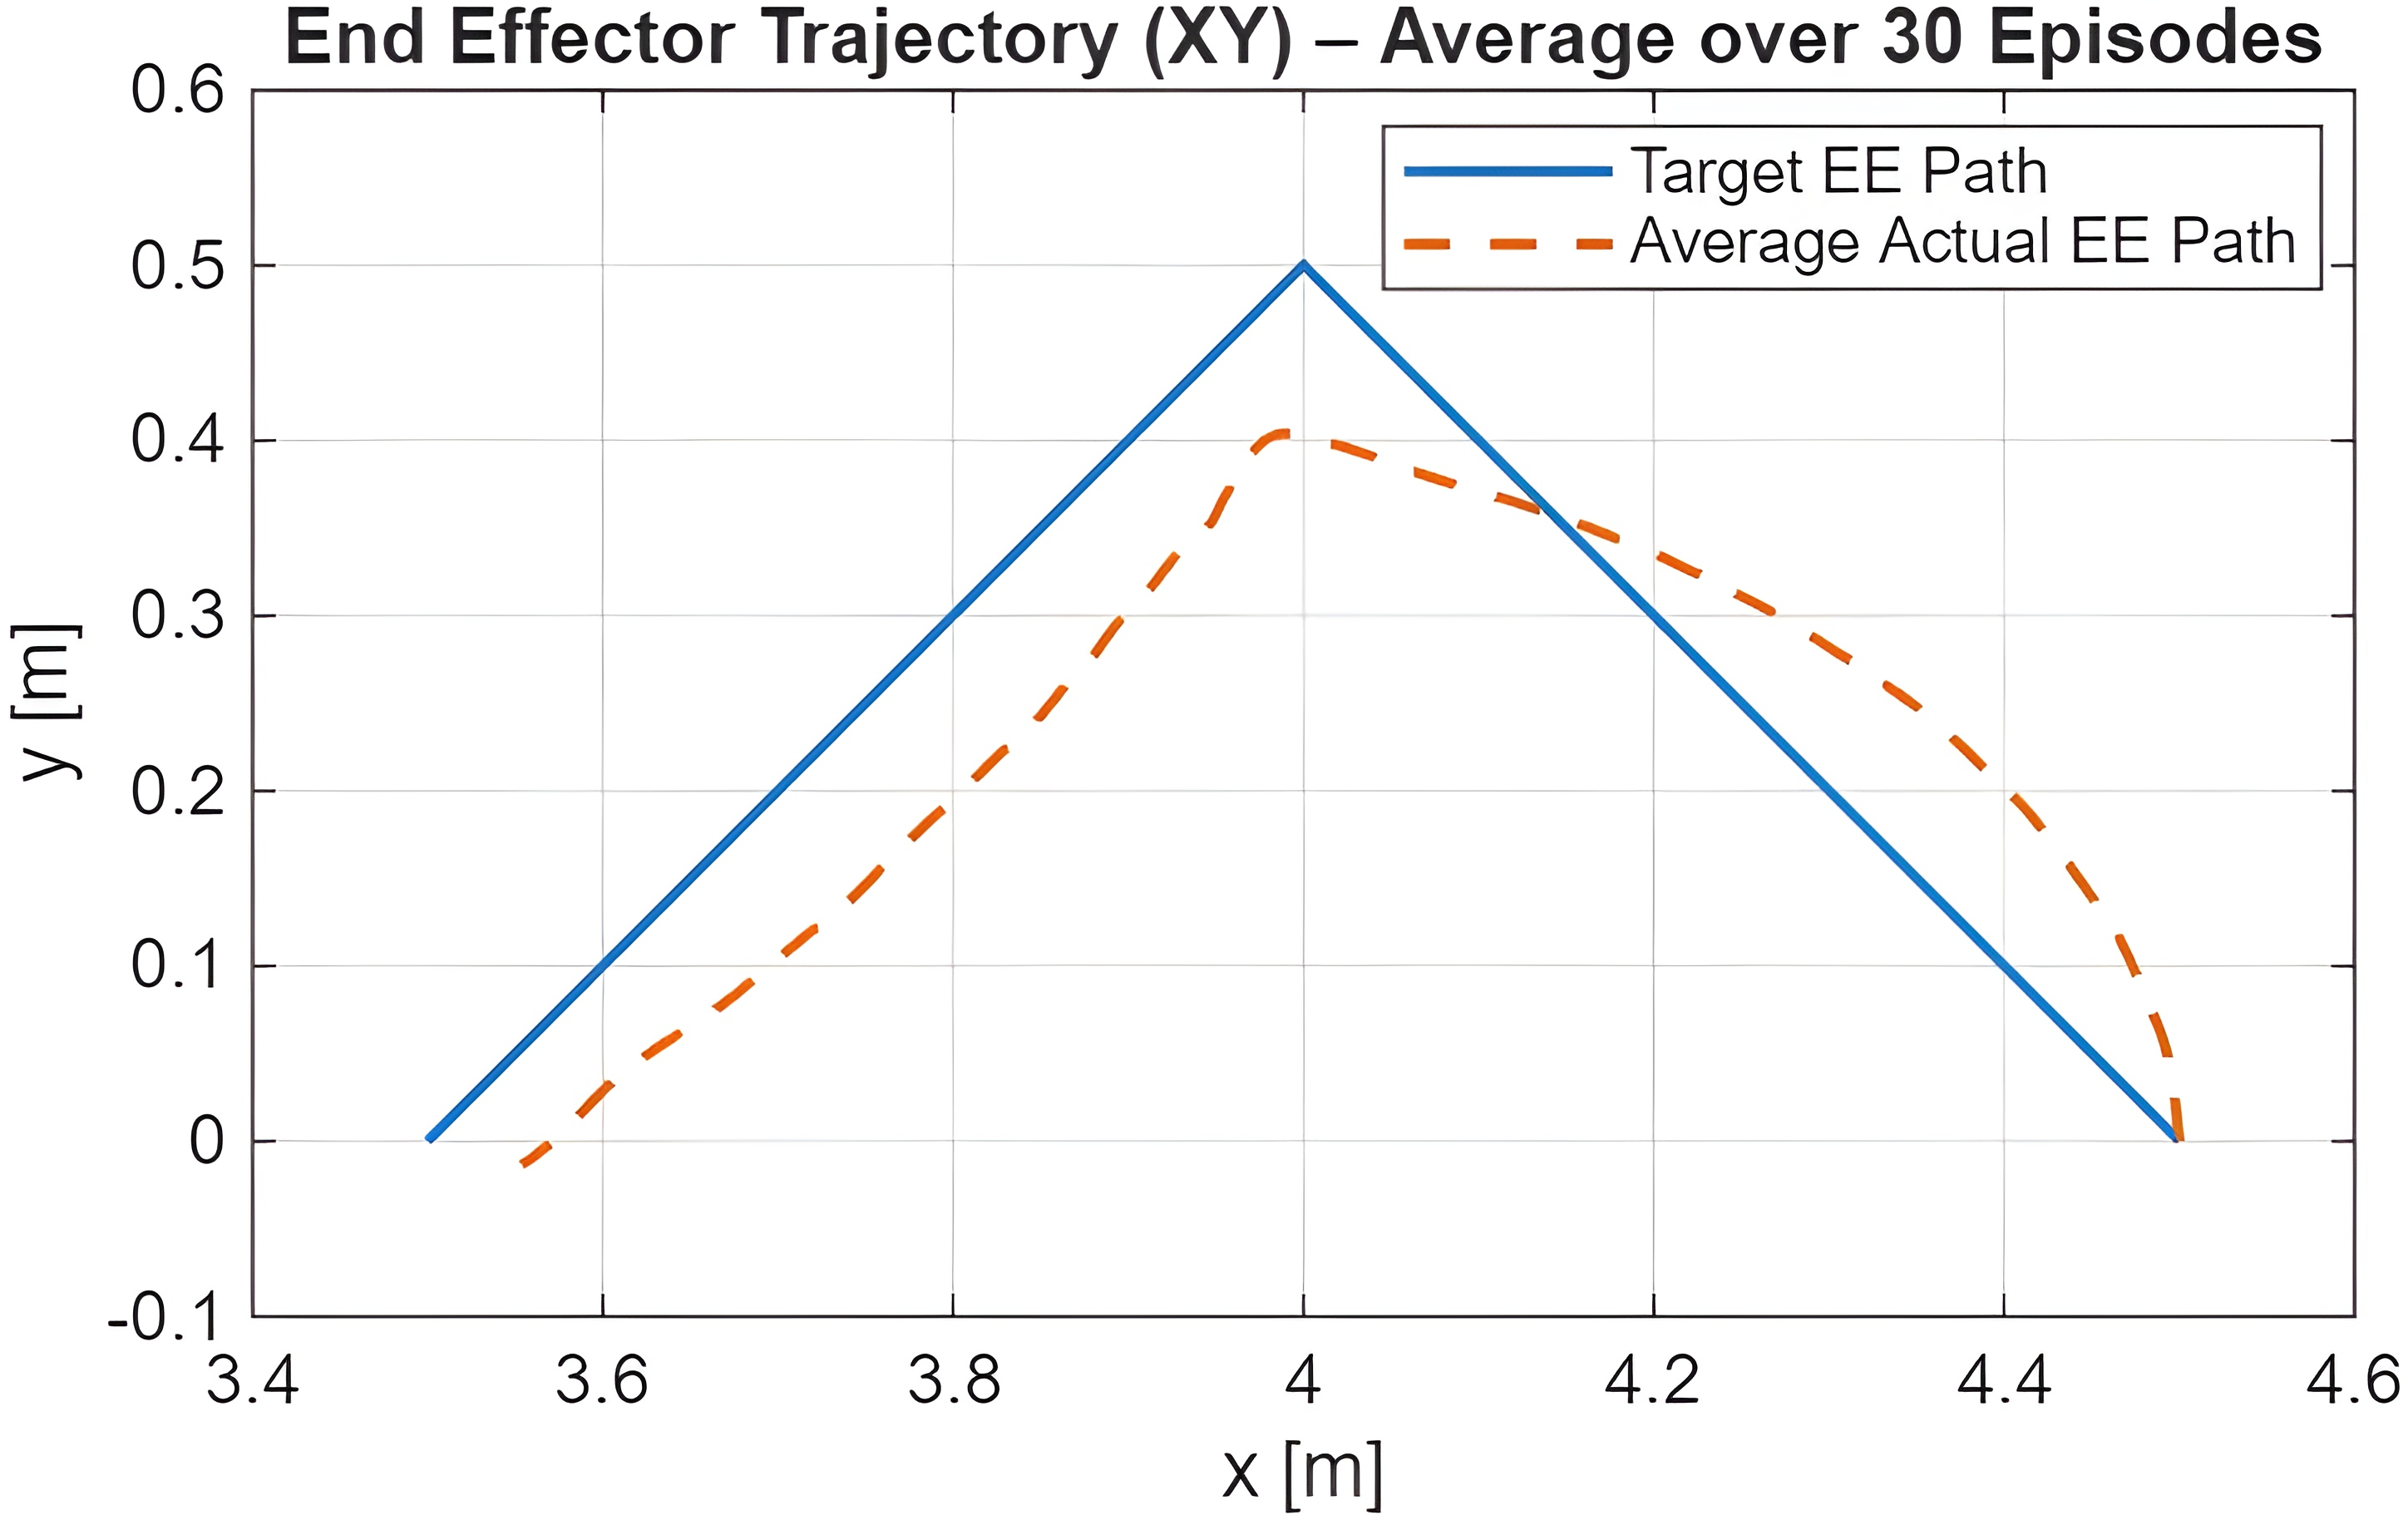
\includegraphics[width=\linewidth]{Figures/rampe_1.png}
        \caption{PPO (Default)}
        \label{fig:r_traj_default}
    \end{subfigure}
    \hfill
    \begin{subfigure}{0.48\textwidth}
        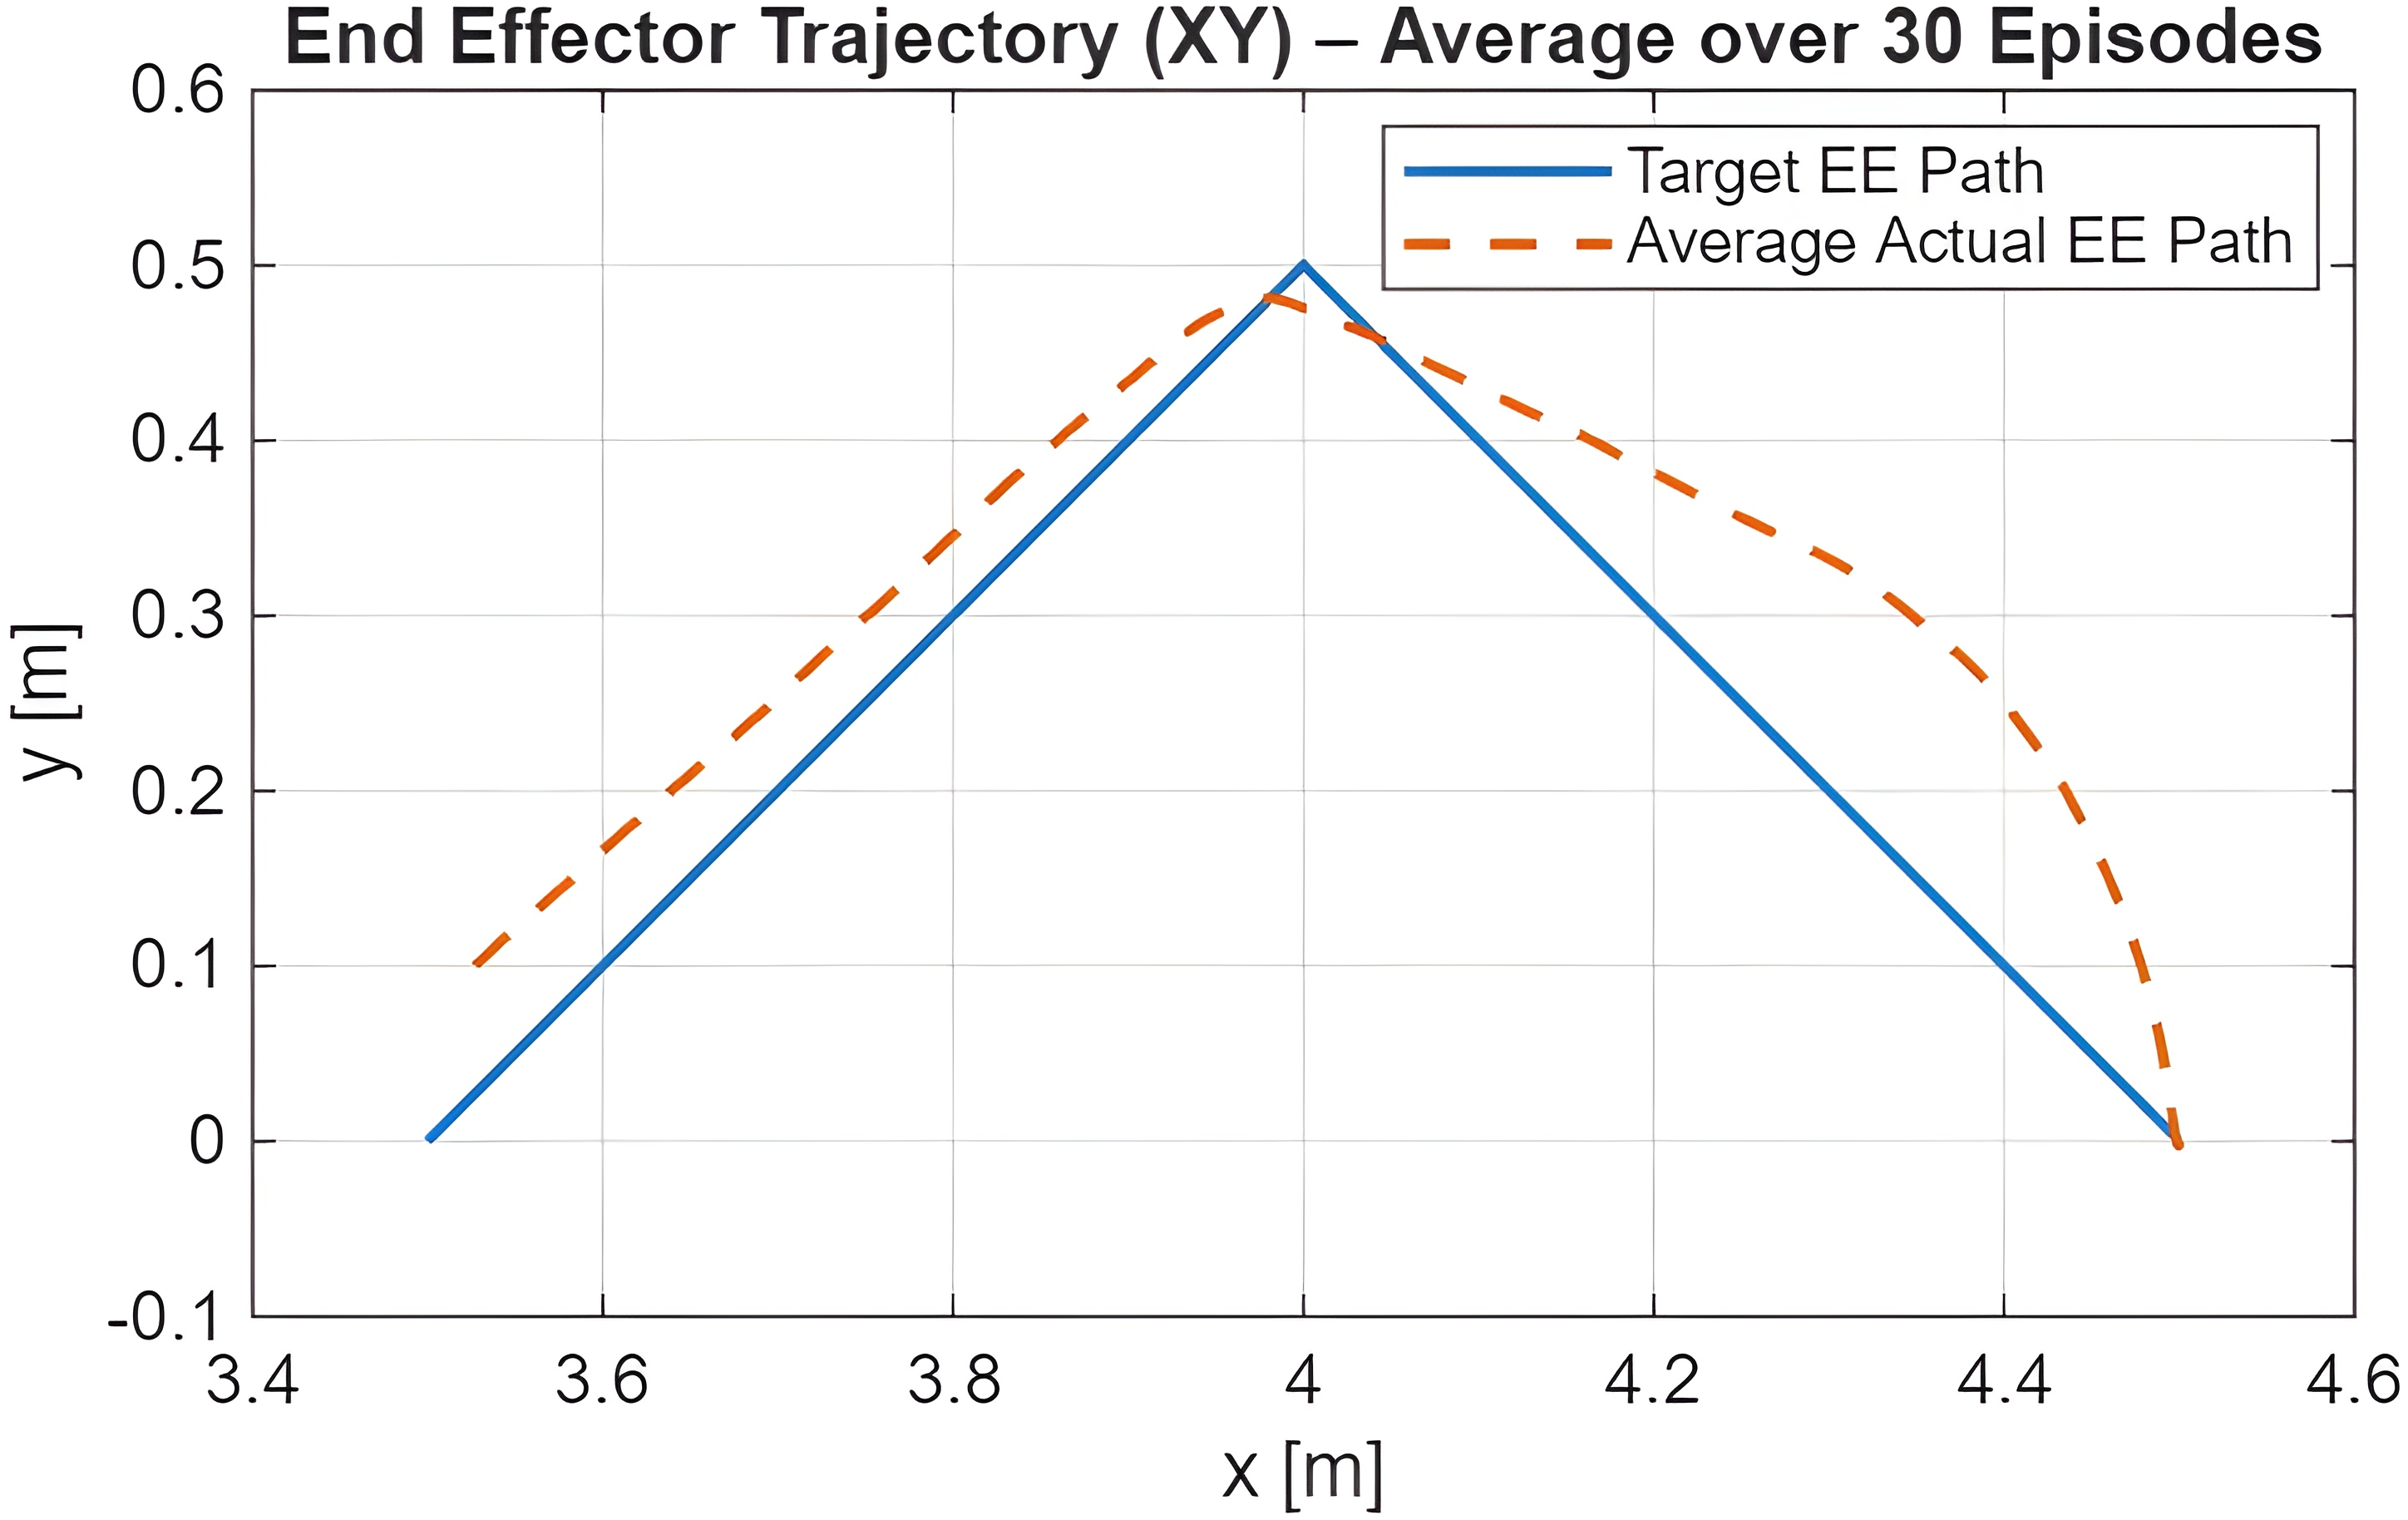
\includegraphics[width=\linewidth]{Figures/rampe_opt_1.png}
        \caption{PPO (Optimized)}
        \label{fig:r_traj_opt}
    \end{subfigure}
    \caption{Target/actual comparison of the piecewise-linear end-effector trajectory in the XY plane.}
    \label{fig:r_trajektorie_xy_compare}
\end{figure*}

\begin{figure*}[!t]
    \centering
    \begin{subfigure}{0.48\textwidth}
        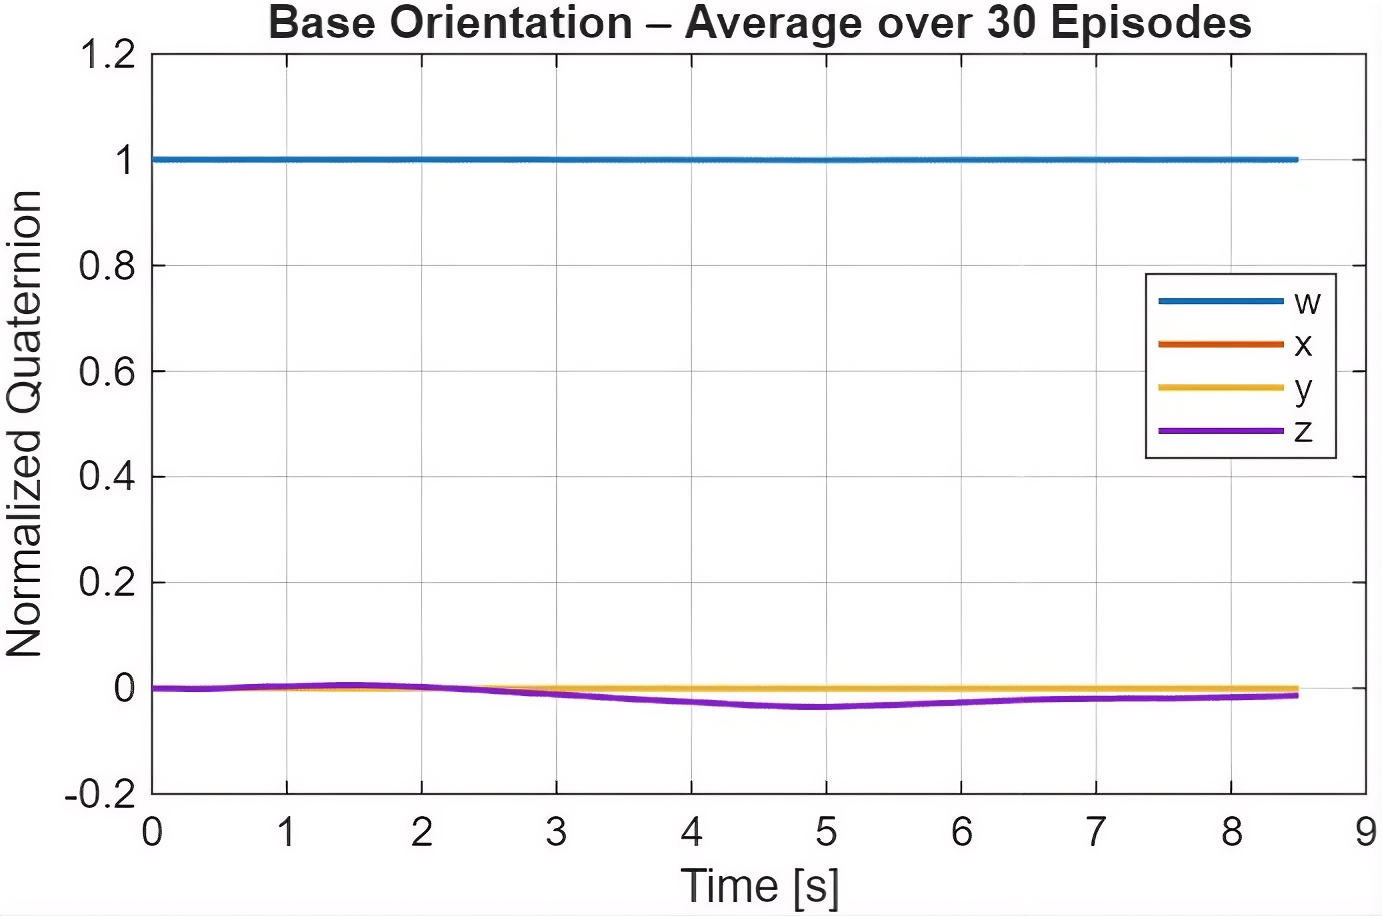
\includegraphics[width=\linewidth]{Figures/basis_ori_1.png}
        \caption{PPO (Default)}
        \label{fig:r_basis_default}
    \end{subfigure}
    \hfill
    \begin{subfigure}{0.48\textwidth}
        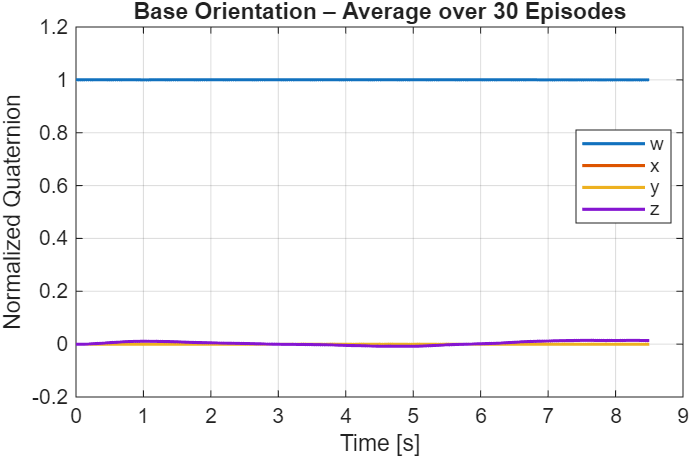
\includegraphics[width=\linewidth]{Figures/basis_ori_opt_1.png}
        \caption{PPO (Optimized)}
        \label{fig:r_basis_opt}
    \end{subfigure}
    \caption{Time evolution of the base orientation (quaternion components) during a test episode with a piecewise-linear trajectory.}
    \label{fig:r_basis_orientation_compare}
\end{figure*}
\textbf{Results.} Table~\ref{tab:ppo_linear_kpi} reports the KPI averages over $N_{\mathrm{eval}} = 30$ evaluation episodes for PPO with the default and the optimized configurations on the piecewise-linear reference. The optimized PPO increases the episodic return ($K_1$: $-0.4565 \to -0.2977$), reduces the base attitude disturbance ($K_4$ decreases by approximately $44\%$, see~\autoref{fig:r_basis_orientation_compare}), reduces the residual base angular velocity ($K_8$ decreases by approximately $15\%$), and reduces the energy consumption ($K_9$ decreases by approximately $35\%$). The mean and peak tracking errors ($K_2$ and $K_3$) remain close to those of the default configuration, with a small reduction of the mean error (see~\autoref{fig:r_trajektorie_xy_compare}). The control smoothness metric $K_7$, however, is worse than for the default PPO. This indicates that the hyperparameter configuration tuned for circular tracking does not fully transfer to piecewise-linear references. A direct mitigation is to include a mixture of reference types (circular, linear, and hybrid trajectories) during training or during the hyperparameter search.

\begin{table}[!b]
\centering
\caption{Generalization test on a piecewise-linear end-effector trajectory (two-segment path). Values are 
averaged over $N_{eval}=30$ episodes. Bold indicates the better value according to the KPI definition (K1 higher is better; K2--K9 lower is better).}
\label{tab:ppo_linear_kpi}
\renewcommand{\arraystretch}{1.2}
\setlength{\tabcolsep}{3pt}
\begin{tabular}{lcc}
\toprule
\textbf{Metric (KPI)} & \textbf{PPO (Default)} & \textbf{PPO (Optimized)} \\
\midrule
Mean Episodic Reward (K1)            & $-0.4565$ & $\mathbf{-0.2977}$ \\
Mean Squared EE Position Error (K2)  & 0.0078 & \textbf{0.0070} \\
Max EE Position Error (K3)           & 0.2037 & \textbf{0.2036} \\
Mean Base Orientation Error (K4)     & 0.0412 & \textbf{0.0231} \\
Collision Rate (K5)                 & 0 & 0 \\
Joint Limit Violation Rate (K6)     & 0 & 0 \\
Control Smoothness (K7, jerk)       & \textbf{0.5520} & 0.6839 \\
Mean Base Angular Velocity (K8)      & 0.0399 & \textbf{0.0339} \\
Energy Consumption (K9)              & 7.7144 & \textbf{5.0341} \\
\bottomrule
\end{tabular}
\end{table}


Both the circular and the piecewise-linear evaluations support the use of systematic hyperparameter tuning and tailored network design for safety-critical space-robot control. The piecewise-linear results also show that trajectory-specific tuning may be required to maintain control smoothness across reference geometries.

The following section discusses the implications, limitations, and future steps toward deployment on physical testbeds for space robotics.

\section{Discussion and Conclusion}
\begin{rtwohl}
\hltwo{[R2.14]} This work has investigated the application of continuous deep reinforcement learning to the control of a free-floating space robotic arm, with an emphasis on safety and performance. The results show that an RL-based controller can perform the considered manipulation task in the simulated space environment under the stated assumptions. The optimized PPO agent yields a mean squared end-effector tracking error of $K_2 = 0.0083$, a reduction of $67.7\%$ relative to the default configuration ($K_2 = 0.0257$); the mean base-orientation error decreases by a factor of approximately three ($K_4$: $0.0667 \to 0.022$), and the mean base angular velocity is halved ($K_8$: $0.095\,\mathrm{rad/s} \to 0.050\,\mathrm{rad/s}$). No safety violations were recorded over the 30 evaluation episodes ($K_5 = K_6 = 0$), compared with a $5.1\%$ joint-limit violation rate for the default configuration. Torque smoothness improves by $48.5\%$ ($K_7$) and energy consumption decreases by $16\%$ ($K_9$). These effects are observed together in the reported evaluation rather than as an apparent trade-off between the selected objectives \cite{b1,b7}.
\end{rtwohl}

\begin{rtwohl}
\hltwo{[R2.14]} An additional evaluation was carried out on a piecewise-linear end-effector reference to assess trajectory generalization. The optimized PPO agent outperforms the default configuration on most metrics (return $K_1$: $-0.4565 \to -0.2977$; base-orientation error $K_4$: $-44\%$; energy $K_9$: $-35\%$), which indicates partial transfer of the learned policy. The control-smoothness metric $K_7$, however, is worse than for the default configuration, showing that the hyperparameter configuration tuned for circular tracking does not fully transfer to piecewise-linear references. This motivates either trajectory-diverse training or trajectory-specific tuning to support generalization across reference geometries \cite{b8}.
\end{rtwohl}

\textbf{Practical Implications.} The performance of PPO and TRPO on this task indicates that policy-gradient methods with constrained updates are suitable candidates for continuous control tasks with strong dynamic coupling and safety constraints. The clipped surrogate objective of PPO provides bounded policy updates under the nonlinear free-floating dynamics. The integrated safety components (collision monitor, joint-limit assertion, torque-bound verification) act as a runtime shield during training: they terminate episodes in which the policy would violate a monitored constraint and apply a terminal penalty \cite{b15,b23,b22}. Combined with the penalty-driven reward, this leads to a final policy that respects the monitored constraints in the reported evaluation. For deployment on a physical system, this suggests that safety checks embedded in the training simulator may remain useful at runtime, provided that the deployed system stays within the simulator's fidelity range \cite{b22,b24}.


\begin{rthreehl}
\hlthree{[R3.9]} \textbf{Limitations and Future Work:}
Several limitations should be acknowledged. First, a \emph{sim-to-real gap} remains. Beyond the idealizing assumptions stated in \autoref{sec:sim} (no sensor noise, no latency, rigid body model, no external disturbances), real deployment introduces additional challenges: (a)~\emph{domain shift} due to inaccuracies in the identified mass and inertia parameters, joint friction, and link flexibility not captured in the URDF model; (b)~\emph{onboard compute constraints}, as the learned neural network policy must execute in real time on embedded space-qualified hardware (typically ARM-based processors with limited floating-point throughput), whereas training was performed on a workstation-class CPU; and (c)~\emph{sensor-actuator latency}, where non-negligible delays between state measurement and torque application can destabilize a policy trained under the zero-latency assumption. Mitigating these effects requires domain randomization over simulation parameters, latency injection during training, and ultimately hardware-in-the-loop (HIL) validation~\cite{b8,b22}.
Second, the RL agent exhibits \emph{hyperparameter sensitivity}---the tuned PPO configuration is task-specific and may require re-tuning for different
trajectories or mission scenarios. Third, the \emph{state representation} was manually designed; learned representations or recurrent architectures (LSTM)
might improve performance under partial observability. Fourth, the \emph{safety monitoring} covers targeted critical properties but does not constitute
exhaustive formal verification of the full mission~\cite{b5,b22}. Finally, \emph{no hardware testing} was performed; real-time computation limits,
communication delays, and physical interactions remain to be validated on physical testbeds.

Future work should address these gaps through: (i)~domain randomization over simulation parameters and latency injection to improve sim-to-real robustness~\cite{b8} (see \cref{fig:oos}); (ii)~extension to more complex tasks such as dual-arm coordination, on-orbit assembly, or active debris removal; (iii)~advanced
RL architectures (recurrent policies, attention mechanisms) and safe RL algorithms with explicit constraint handling via Lagrange multipliers
or barrier functions~\cite{b22,b24,b23,b34}; and (iv)~hardware-in-the-loop validation on the authors' testbed for In-Space Robotized Services (IROS) with virtually simulated microgravity and predicted energy consumption (see \cref{fig:oos}).
\end{rthreehl}


\begin{rtwohl}
\hltwo{[R2.14]} \textbf{Conclusion.} This work has presented a framework that combines deep reinforcement learning, multibody simulation, and formal-methods-based safety monitoring for Cartesian path tracking of a free-floating space robot. A comparison of six continuous-action RL algorithms under unified conditions identified PPO as the algorithm with the most favourable trade-off between tracking accuracy, base disturbance, and training stability for the considered task. Subsequent hyperparameter tuning and network tailoring of the PPO agent yielded a policy that, relative to the default PPO configuration, reduces the tracking error by $67.7\%$, reduces the base-orientation error by a factor of approximately three, shows no joint-limit or collision violations over 30 evaluation episodes, and reduces the energy consumption by $16\%$. The integration
of monitored safety constraints and torque-bound verification into the training loop helped keep these results
within the defined safety envelope, addressing part of the typical black-box
nature of learned controllers. These findings, grounded in quantitative experimental evidence,
support further investigation of safety-augmented deep RL for safety-critical space manipulation tasks.
\end{rtwohl}



The results also illustrate the influence of algorithm choice and parameter tuning on learning performance for the considered task. They support the view that no single RL algorithm is uniformly best across applications: under unified conditions, the choice of algorithm, network architecture, and hyperparameter setting visibly affects the achieved tracking accuracy and base stability. Systematic benchmarking of candidate algorithms is therefore a practical step in the selection of an appropriate RL controller for a given task.

While several open problems remain for real-world deployment, the proposed framework provides a basis for further investigation. Possible application areas include satellite servicing, on-orbit assembly, and active debris removal, where learning-based controllers can adapt to uncertain dynamics within predefined operational limits. The combination of an RL policy with a separate runtime layer that monitors and, where required, overrides commands violating the specified constraints is one realization of such an architecture; in this combination, the learned policy provides adaptability, while the monitoring layer enforces the specified safety-critical properties~\cite{b1,b23}.

%\begin{figure}[!t]
%	\centering
%	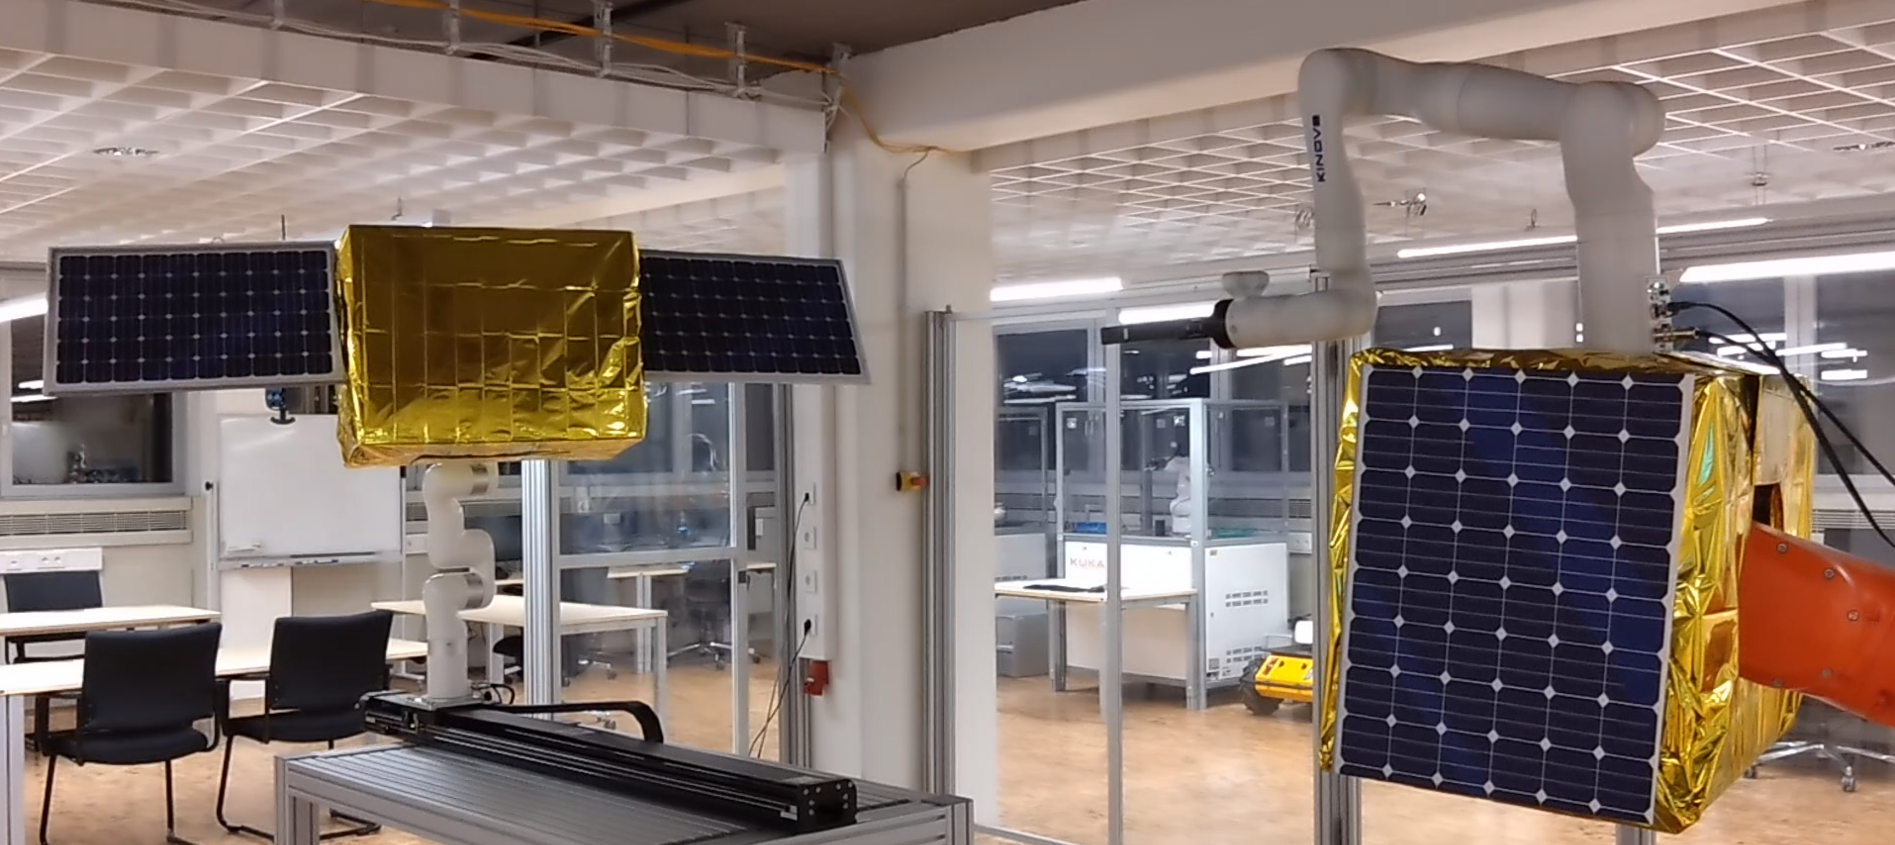
\includegraphics[width=0.8\linewidth]{Figures/testbed.png}
%	\caption{Our testbed for In-Space Robotized Services.}
%	\label{fig:physicaltestbed}
%\end{figure}

\begin{figure}[!t]
	\centering
	\begin{subfigure}{0.99\columnwidth}
		\centering
		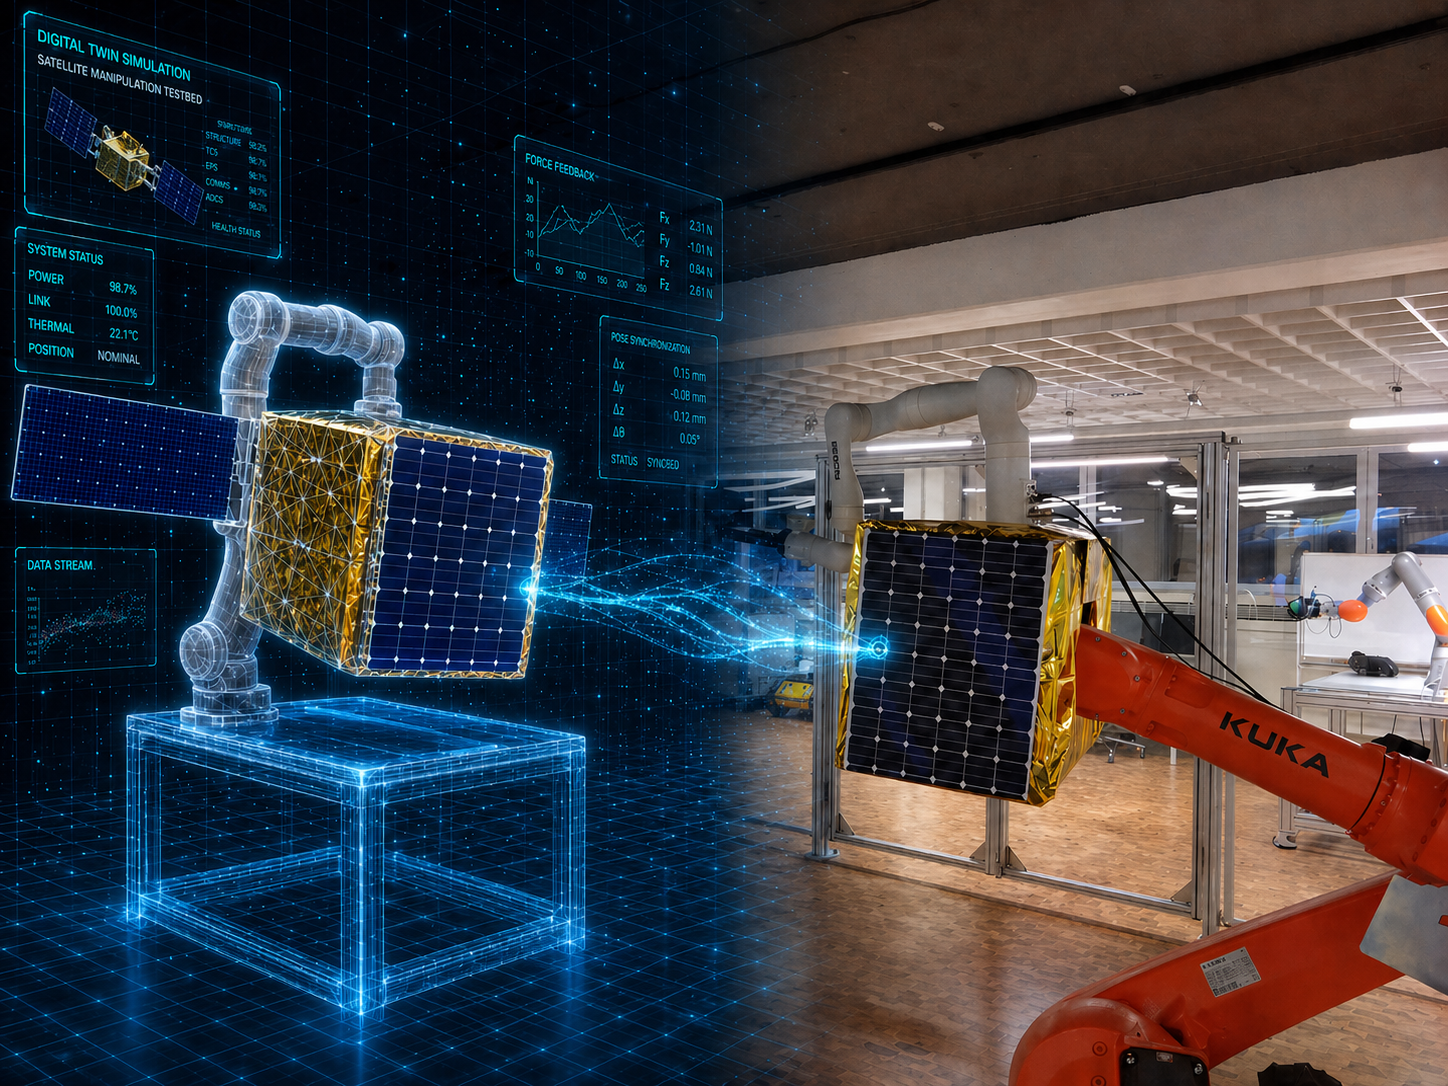
\includegraphics[width=\linewidth]{Figures/oos1.png}
	\end{subfigure}
	\caption{Gradual hybrid testbeds integrate AI-driven digital twins (left) with physical robotic systems (right), providing a framework for studying policy optimization and domain-randomization strategies for sim-to-real transfer. Illustration created using a picture of the physical setup at frankfurt university of applied sciences
		and with the help of GPT-Image-2.}
	\label{fig:oos}
\end{figure}

The present study contributes one step in this direction. Future research at the intersection of robotics, reinforcement learning, and formal methods is required to extend the present results to physical deployment and to broader mission scenarios.

\section*{Acknowledgment}
The authors used DeepL Translator/Write~\cite{deeplTr,deeplWr} and OpenAI ChatGPT~\cite{openai_chatgpt} solely for language editing and grammar enhancement. 
All technical content and conclusions were created and verified by the authors.

\begin{thebibliography}{00}

\bibitem{b1}
A. Flores-Abad, O. Ma, K. Pham, and S. Ulrich, ``A review of space robotics technologies for on-orbit servicing,'' \emph{Prog. Aerosp. Sci.}, vol.~68, pp. 1--26, 2014, doi: 10.1016/j.paerosci.2014.03.002.



\bibitem{b6}
K. Nanos and E. G. Papadopoulos, ``On the dynamics and control of free-floating space manipulator systems in the presence of angular momentum,'' \emph{Front. Robot. AI}, vol.~4, p.~26, 2017, doi: 10.3389/frobt.2017.00026.



\bibitem{b11}
E. Papadopoulos, I. Kaliakatsos, and D. Psarros, ``Minimum fuel techniques for a space robot simulator with a reaction wheel and PWM thrusters,'' in \emph{Proc. Eur. Control Conf. (ECC)}, 2007, pp. 3391--3398.



\bibitem{b32}
E. Papadopoulos and A. Abu-Abed, ``Design and motion planning for a zero-reaction manipulator,'' in \emph{Proc. IEEE Int. Conf. Robot. Autom. (ICRA)}, 1994, pp. 1554--1559, doi: 10.1109/ROBOT.1994.351367.



\bibitem{muhlbauer2025software}
M. M{\"u}hlbauer, M. Chalon, M. Ulmer, and A. Albu-Sch{\"a}ffer, ``Software for the SpaceDREAM robotic arm,'' in \emph{Proc. IEEE Aerosp. Conf.}, 2025.



\bibitem{rybus2024robotic}
T. Rybus, ``Robotic manipulators for in-orbit servicing and active debris removal: Review and comparison,'' \emph{Prog. Aerosp. Sci.}, vol.~151, p.~104550, 2024.



%\bibitem{maurenbrecher2024robograv}
%H. Maurenbrecher \emph{et al.}, ``RoboGrav---Towards force sensitive space manipulators,'' in \emph{Proc. I-SAIRAS}, 2024.

\bibitem{kaigom2011optimal}
E. Guiffo Kaigom, T. Jung, and J. Roßmann, ``Optimal motion planning of a space robot with base disturbance minimization,'' in \emph{Proc. 11th Symp. Adv. Space Technol. Robot. Autom.}, 2011.

\bibitem{kaigom2025deep}
E. Guiffo Kaigom, ``Deep generative and discriminative digital twin endowed with variational autoencoder for unsupervised predictive thermal condition monitoring of physical robots in Industry 6.0 and Society 6.0,'' \emph{IFAC-PapersOnLine}, vol.~59, pp. 7--12, 2025.

\bibitem{huang2023obstacle}
Z. Huang, G. Chen, Y. Shen, R. Wang, C. Liu, and L. Zhang, ``An obstacle-avoidance motion planning method for redundant space robot via reinforcement learning,'' \emph{Actuators}, vol.~12, no.~2, p.~69, 2023.



\bibitem{al2024reinforcement}
A. Al Ali and Z. Zhu, ``Reinforcement learning for path planning of free-floating space robotic manipulator with collision avoidance and observation noise,'' \emph{Front. Control Eng.}, vol.~5, p.~1394668, 2024.



\bibitem{d2024failure}
M. D'Ambrosio, L. Capra, A. Brandonisio, and M. Lavagna, ``Failure management via deep reinforcement learning for robotic in-orbit servicing,'' in \emph{Proc. SPAICE---1st Joint ESA/IAA Conf. AI Space}, 2024, pp. 335--339.



\bibitem{al2024path}
A. Al Ali, J. Shi, and Z. Zhu, ``Path planning of 6-DOF free-floating space robotic manipulators using reinforcement learning,'' \emph{Acta Astronaut.}, vol.~224, pp. 367--378, 2024.



\bibitem{hu2025deep}
Y. Hu, D. Zhou, W. Yao, X. Shao, and G. Sun, ``Deep reinforcement learning-based trajectory planning with continuous pose representation for 6-DoF free-floating space robot,'' \emph{Aerosp. Sci. Technol.}, p.~110540, 2025.



\bibitem{zhang2025learning}
O. Zhang, Z. Liu, X. Shao, W. Yao, L. Wu, and J. Liu, ``Learning-based task space trajectory planning framework with pre-planning and post-processing for uncertain free-floating space robots,'' \emph{IEEE Trans. Aerosp. Electron. Syst.}, early access, 2025.



\bibitem{wei2025trajectory}
Y. Wei, X. Bai, and H. Lu, ``Trajectory planning of free-floating space robot for non-cooperative tumbling target capture based on deep reinforcement learning,'' \emph{Robotica}, vol.~43, pp. 2674--2692, 2025.



\bibitem{wu2020reinforcement}
Y. Wu, Z. Yu, C. Li, M. He, B. Hua, and Z. Chen, ``Reinforcement learning in dual-arm trajectory planning for a free-floating space robot,'' \emph{Aerosp. Sci. Technol.}, vol.~98, p.~105657, 2020.



\bibitem{b14}
J. Schulman, S. Levine, P. Abbeel, M. Jordan, and P. Moritz, ``Trust region policy optimization,'' in \emph{Proc. Int. Conf. Mach. Learn. (ICML)}, 2015, pp. 1889--1897.



\bibitem{b17}
S. Fujimoto, H. van Hoof, and D. Meger, ``Addressing function approximation error in actor-critic methods,'' in \emph{Proc. Int. Conf. Mach. Learn. (ICML)}, 2018, pp. 1587--1596.



\bibitem{b18}
T. Haarnoja, A. Zhou, P. Abbeel, and S. Levine, ``Soft actor-critic: Off-policy maximum entropy deep reinforcement learning with a stochastic actor,'' in \emph{Proc. Int. Conf. Mach. Learn. (ICML)}, 2018, pp. 1861--1870.



\bibitem{b15}
J. Schulman, F. Wolski, P. Dhariwal, A. Radford, and O. Klimov, ``Proximal policy optimization algorithms,'' arXiv:1707.06347, 2017.



\bibitem{b21}
R. J. Williams, ``Simple statistical gradient-following algorithms for connectionist reinforcement learning,'' \emph{Mach. Learn.}, vol.~8, pp. 229--256, 1992.



\bibitem{b7}
R. S. Sutton and A. G. Barto, \emph{Reinforcement Learning: An Introduction}, 2nd~ed. Cambridge, MA, USA: MIT Press, 2018.



\bibitem{b5}
MathWorks, ``Simulink Design Verifier,'' The MathWorks, Inc., Natick, MA, USA, 2024. [Online]. Available: \url{https://www.mathworks.com/help/sldv/}



\bibitem{b22}
J. Garc{\'\i}a and F. Fern{\'a}ndez, ``A comprehensive survey on safe reinforcement learning,'' \emph{J. Mach. Learn. Res.}, vol.~16, pp. 1437--1480, 2015.



\bibitem{b23}
M. Alshiekh, R. Bloem, R. Ehlers, B. K{\"o}nighofer, S. Niekum, and U. Topcu, ``Safe reinforcement learning via shielding,'' in \emph{Proc. AAAI Conf. Artif. Intell.}, 2018, pp. 2669--2678.



\bibitem{b25}
Open Robotics, ``URDF (Unified Robot Description Format),'' ROS~2 Documentation, 2024. [Online]. Available: \url{https://docs.ros.org/en/rolling/Tutorials/Intermediate/URDF/URDF-Main.html}



\bibitem{b26}
MathWorks, ``Import URDF models,'' MATLAB \& Simulink Documentation, 2024. [Online]. Available: \url{https://www.mathworks.com/help/sm/ug/urdf-import.html}



\bibitem{b27}
MathWorks, ``smimport---Import a CAD, URDF, or Robotics System Toolbox model,'' MATLAB \& Simulink Documentation, 2024. [Online]. Available: \url{https://www.mathworks.com/help/sm/ref/smimport.html}



\bibitem{b28}
MathWorks, ``Mechanism Configuration,'' MATLAB \& Simulink Documentation, 2024. [Online]. Available: \url{https://www.mathworks.com/help/sm/ref/mechanismconfiguration.html}



\bibitem{b2}
J. Kober, J. A. Bagnell, and J. Peters, ``Reinforcement learning in robotics: A survey,'' \emph{Int. J. Robot. Res.}, vol.~32, no.~11, pp. 1238--1274, 2013.



\bibitem{b24}
J. Achiam, D. Held, A. Tamar, and P. Abbeel, ``Constrained policy optimization,'' in \emph{Proc. Int. Conf. Mach. Learn. (ICML)}, 2017, pp. 22--31.



\bibitem{b34}
A. D. Ames, S. Coogan, M. Egerstedt, G. Notomista, K. Sreenath, and P. Tabuada, ``Control barrier functions: Theory and applications,'' in \emph{Proc. Eur. Control Conf. (ECC)}, 2019, pp. 3420--3431.



\bibitem{leutert2024ai}
F. Leutert \emph{et al.}, ``AI-enabled cyber--physical in-orbit factory---AI approaches based on digital twin technology for robotic small satellite production,'' \emph{Acta Astronaut.}, vol.~217, pp. 1--17, 2024.



\bibitem{muhlbauer2025towards}
M. M{\"u}hlbauer \emph{et al.}, ``Towards an in-orbit cubesat factory,'' in \emph{Proc. 76th Int. Astronaut. Congr. (IAC)}, 2025.



\bibitem{maqbool2025systems}
O. Maqbool and J. Roßmann, ``Systems aware scenario engineering for life cycle-spanning verification and validation of complex CPS,'' Authorea Preprints, 2025. [Online]. Available: \url{https://www.authorea.com}



\bibitem{b9}
J. Virgili-Llop, ``SPART: Spacecraft Robotics Toolkit,'' 2017. [Online]. Available: \url{https://github.com/NPS-SRL/SPART}



\bibitem{b12}
E. Ribeiro, R. Mendes, M. Terra, and V. Grassi, ``Dynamic parameter identification of a 7-DoF lightweight robot manipulator using probabilistic differential optimization,'' in \emph{Proc. IEEE Int. Conf. Syst., Man, Cybern. (SMC)}, 2022, pp. 1917--1923.



\bibitem{b3}
MathWorks, ``6-DOF Joint (Simscape Multibody),'' MATLAB \& Simulink Documentation, 2024. [Online]. Available: \url{https://www.mathworks.com/help/sm/ref/6dofjoint.html}



\bibitem{b31}
MathWorks, ``Spatial Contact Force,'' MATLAB \& Simulink Documentation, 2024. [Online]. Available: \url{https://www.mathworks.com/help/sm/ref/spatialcontactforce.html}



\bibitem{b29}
MathWorks, ``Solver Configuration,'' MATLAB \& Simulink Documentation, 2024. [Online]. Available: \url{https://www.mathworks.com/help/simscape/ref/solverconfiguration.html}



\bibitem{b30}
MathWorks, ``Fixed-step size (fundamental sample time),'' MATLAB \& Simulink Documentation, 2024. [Online]. Available: \url{https://www.mathworks.com/help/simulink/gui/fixedstepsizefundamentalsampletime.html}



\bibitem{b4}
MathWorks, ``Reinforcement Learning Toolbox---rlPPOAgent,'' MATLAB \& Simulink Documentation, 2024. [Online]. Available: \url{https://www.mathworks.com/help/reinforcement-learning/ref/rl.agent.rlppoagent.html}



\bibitem{b16}
T. P. Lillicrap \emph{et al.}, ``Continuous control with deep reinforcement learning,'' in \emph{Proc. Int. Conf. Learn. Represent. (ICLR)}, 2016.



\bibitem{b8}
J. Tobin, R. Fong, A. Ray, J. Schneider, W. Zaremba, and P. Abbeel, ``Domain randomization for transferring deep neural networks from simulation to the real world,'' in \emph{Proc. IEEE/RSJ Int. Conf. Intell. Robots Syst. (IROS)}, 2017, pp. 23--30.


\bibitem{deeplTr}
DeepL SE, ``DeepL Translator,'' [Online]. Available: \url{https://www.deepl.com/de/translator}

\bibitem{deeplWr}
DeepL SE, ``DeepL Write,'' [Online]. Available: \url{https://www.deepl.com/de/write}


\bibitem{openai_chatgpt}
OpenAI, ``ChatGPT,'' [Online]. Available: \url{https://chat.openai.com}



\bibitem{todorov2012mujoco}
E. Todorov, T. Erez, and Y. Tassa, ``MuJoCo: A physics engine for model-based control,'' in \emph{Proc. IEEE/RSJ Int. Conf. Intell. Robots Syst. (IROS)}, 2012, pp. 5026--5033.



\bibitem{koenig2004gazebo}
N. Koenig and A. Howard, ``Design and use paradigms for Gazebo, an open-source multi-robot simulator,'' in \emph{Proc. IEEE/RSJ Int. Conf. Intell. Robots Syst. (IROS)}, vol. 3, 2004, pp. 2149--2154.



\bibitem{korber2021comparing}
M. K\"orber, J. Lange, S. Rediske, S. Steinmann, and R. Gl\"uck, ``Comparing popular simulation environments in the scope of robotics and reinforcement learning,'' arXiv preprint arXiv:2103.04616, 2021.



\bibitem{collins2021review}
J. Collins, S. Chand, A. Vanderkop, and D. Howard, ``A review of physics simulators for robotic applications,'' \emph{IEEE Access}, vol. 9, pp. 51416--51431, 2021.



\end{thebibliography}

\begin{IEEEbiography}[{
\includegraphics[width=1in,height=1.25in,clip,keepaspectratio]{Figures/Bewerbungsfoto_Ermisch.jpg}}]{Patrick S. Ermisch}
Patrick S. Ermisch was born in Frankfurt am Main, Germany, on December 18, 2002. He received the Abitur degree and 
is currently pursuing the B.Eng. degree in mechatronics at Frankfurt University of Applied Sciences, Frankfurt, 
Germany, with an expected graduation in 2026. His major field of study is mechatronics.

He has gained practical experience through an internship at SEW-EURODRIVE, where he contributed to the further 
development of a mobile application for the manual control of logistics robots. In addition, he worked as a tutor 
for Physics~I and Physics~II and as a student research assistant, supporting research on particle simulation and 
the development of an application for visualization and simulation purposes. His research interests include 
reinforcement learning for robotics, space robotic systems, and simulation-based control methods.

Mr.\ Ermisch has been listed on the Dean’s List of Frankfurt University of Applied Sciences multiple times in 
recognition of his academic performance.
\end{IEEEbiography}



\begin{IEEEbiography}[{
\includegraphics[width=1in,height=1.25in,clip,keepaspectratio]{Figures/egk.jpg}}]{Eric Guiffo Kaigom} was born in Douala, Cameroon. He received the Dipl.-Ing. and \mbox{Dr.-Ing.} (summa cum laude) degrees in electrical engineering from RWTH Aachen University, Aachen, Germany. He was a Research Associate with the Institute for Man-Machine Interaction at RWTH Aachen University, where he led the ``Intelligent Robots'' team and coordinated technology development and transfer activities with partners in robotics-based manufacturing and on-orbit servicing, including projects funded under the European Union's Horizon 2020 and In-Space Automation programs. He then worked in industry as Head of Emerging Technologies. He is currently a Full Professor with Frankfurt University of Applied Sciences, Frankfurt, Germany. His research interests include robotics, digital twins, and artificial intelligence $\slash$ machine learning. 
\end{IEEEbiography}

\EOD

\end{document}
